% Esta plantilla ha sido diseñada por Daniel del Río Velilla, profesor en la Escuela de Aeronáutica y del Espacio, UPM.
% LA PLANTILLA ES DE USO LIBRE PERO ESTÁ SUJETA A DERECHOS DE PROPIEDAD INTELECTUAL, POR LO QUE SU COMERCIALIZACIÓN ES ILEGAL.

% Plantilla Modificada por Iván Moya
% Plantilla Trabajos etsiae

\documentclass[11pt,a4paper,titlepage,twoside]{report}

%   ---   DEFINICION DEL TRABAJO   ---   %

\newcommand{\Project}{Fabricación Aeroespacial}
\newcommand{\ProjectTitle}{Práctica de Soldadura y Chapistería}
\newcommand{\ProjectSubject}{Grado en Ingeniería Aeroespacial}
\newcommand{\ProjectAutor}{Álvarez Capitán, Belén \\ & Linares Mompeón, Lucía \\ & Moya Ortiz, Iván \\ & Rosselló Delporte, Aruna \\ & Varó Torrecillas, Jorge}
\newcommand{\Grupo}{SJ11}
\newcommand{\ProjectLocation}{Madrid}
\newcommand{\ProjectDate}{\today}
% Descomentar si se tiene un repositorio del trabajo
 \newcommand{\ProjectGitHub}{https://github.com/IvanMoyaO/Fabricacion}
\newcommand{\pag}[1]{página \pageref{#1}}
 

%   ---   INCLUIR ARCHIVOS DE CONFIGURACION   ---   %

\usepackage[utf8]{inputenc}         % Permite escribir códigos especiales

% AJUSTES DEL IDIOMA
\usepackage[spanish]{babel}
\decimalpoint
\renewcommand{\spanishtablename}{Tabla}
\addto\extrasenglish{
    \renewcommand{\subsubsectionautorefname}{Section}
    \renewcommand{\subsectionautorefname}{Section}
    \renewcommand{\sectionautorefname}{Section}
}
\usepackage[title]{appendix}
\renewcommand{\appendixname}{Anexos}
\renewcommand{\appendixtocname}{Anexos}
\renewcommand{\appendixpagename}{Anexos}


% GEOMETRIA
\usepackage[paper=A4]{typearea}
\usepackage[includemp,
            top=2 cm,
            left = 1.2 cm, 
            right = 1.2 cm,
            bottom=2 cm,
            headsep = 3.5 cm,
            marginparwidth=2 cm,
            marginparsep=0.4 cm]{geometry}


% INDENTACION
\usepackage{indentfirst}
\setlength{\parskip}{5pt}       
\setlength{\parindent}{0pt}


% ESPACIADO
\usepackage{setspace}
\spacing{1.2}
\let\ph\mlplaceholder % shorter macro


% GENERAR PDF/A y otras cosas del pdf
\usepackage[a-1b]{pdfx}
\usepackage[pdftex]{graphicx}
    \graphicspath{
      {./Figures/Portada_HF/}
      {./Figures/01/}
      {./Figures/02/}
      {./Figures/03/}
      {./Figures/04/}
      {./Figures/05/}
      {./Figures/06/}
      {./Figures/A_01/}
      {./Figures/A_02/}
    }
\usepackage{pdfpages}               % Incluir PDF diferente tamaño


% URLS Y LINKS
\hypersetup{hidelinks}    % Hide borders links
\usepackage{url}
\Urlmuskip=0mu plus 1mu


% EXPRESIONES MATEMATICAS Y SÍMBOLOS
\usepackage{textcomp}               % Symbols in text
\usepackage{amsmath}
\usepackage{amssymb}
\usepackage{mathtools}
\usepackage[T1]{fontenc}
\usepackage{mathtools}
\usepackage{mathrsfs}
\usepackage{derivative}
\usepackage{amsmath,amssymb}
\usepackage{float}
\DeclareMathOperator{\Tr}{Tr}
\usepackage{bigints}
\usepackage{gensymb}    % Para hacer los circulitos de grados
\usepackage{eurosym}
\usepackage{fontawesome}


% INCLUIR CÓDIGO EN EL DOCUMENTO
\usepackage{listings}
\renewcommand{\lstlistingname}{Listado}		% Para que las listas sean es español
%\usepackage[framed,numbered,autolinebreaks,useliterate]{mcode}      % MATLAB CODE
% \lstset{
%     inputencoding=utf8,
%     literate={Á}{{\'A}}1 {á}{{\'a}}1 {É}{{\'E}}1 {é}{{\'e}}1 {Í}{{\'I}}1 {í}{{\'i}}1 {Ó}{{\'O}}1 {ó}{{\'o}}1 {Ú}{{\'U}}1 {ú}{{\'u}}1 
%     }

%\lstset{
%  basicstyle         = \mlttfamily,
%  escapechar         = ",
%}
%\usepackage[numbered]{matlab-prettifier}


% ACRONIMOS
% https://tex.stackexchange.com/questions/25520/how-can-i-use-the-latex-acronym-package-and-optionally-create-an-acronym-list-i
% https://sourceforge.net/p/texstudio/discussion/907839/thread/7ced058c/  -> SI NO APARECEN LOS ACRONIMOS
\usepackage[acronym,smallcaps]{glossaries}[=v4.46]
% ,nonumberlist
% \loadglsentries[\acronymtype]{./Tex_Files/acronyms.tex}
\makeglossaries
%\usepackage{nomencl}
%\makenomenclature
%\usepackage{etoolbox}
%\renewcommand\nomgroup[1]{%
%  \item[\bfseries
%  \ifstrequal{#1}{P}{Propiedades físicas}{%
%  \ifstrequal{#1}{S}{Señales ópticas}{%
%  \ifstrequal{#1}{F}{Fibra óptica}{%
%  \ifstrequal{#1}{C}{Material compuesto}{}}}}%
% ]}


% BIBLIOGRAFÍA
%\usepackage{biblatex}
%\addbibresource{references.bib}
%\setlength\parindent{0pt}


% DISEÑO DE TABLAS Y FIGURAS 
% \usepackage{subfigure}
% \usepackage{subfloat}
\usepackage{caption}
\usepackage{subcaption}		% https://tex.stackexchange.com/questions/295456/texstudio-beginsubfigure-unrecognized-command
\usepackage{svg}
\usepackage{import}
\usepackage{longtable}
\usepackage{multirow}
\usepackage{multicol}
\usepackage{threeparttable}
\usepackage{booktabs}
\usepackage{tabu}
\usepackage{bigstrut}
\usepackage{tabularx}
    \makeatletter
    \def\hlinewd#1{%
    \noalign{\ifnum0=`}\fi\hrule \@height #1 \futurelet
    \reserved@a\@xhline}
    \makeatother
\usepackage{placeins}  %para poder poner Floatbarrier
\usepackage{svg}


% ENUMERACIONES
\usepackage{enumerate}
\usepackage{enumitem}  % Selecionar la forma del item


% NOTAS PIE DE PAGINA
\usepackage[colorinlistoftodos]{todonotes}  % TO DO
\newcommand\blfootnote[1]{%
  \begingroup
  \renewcommand\thefootnote{}\footnote{#1}%
  \addtocounter{footnote}{-1}%
  \endgroup
}


% DEFINICIÓN DE COLORES 
\usepackage{xcolor}
\usepackage{colortbl}


% COMANDOS
\providecommand\phantomsection{}    % Para añadir phantomsections al indice


% LANDSCAPE
\usepackage{pdflscape}
\usepackage{everypage}
\usepackage{lipsum}
% Landscape configuration
\newcommand{\Lpagenumber}{\ifdim\textwidth=\linewidth\else\bgroup
  \dimendef\margin=0 %use \margin instead of \dimen0
  \ifodd\value{page}\margin=\oddsidemargin
  \else\margin=\evensidemargin
  \fi
  \raisebox{\dimexpr -\topmargin-\headheight-\headsep-0.5\linewidth}[0pt][0pt]{%
    \rlap{\hspace{\dimexpr \margin+\textheight+\footskip}}}%
\egroup\fi}
\AddEverypageHook{\Lpagenumber}%
% Code
%\begin{landscape}
% Text
%\end{landscape}


% MISCELANEO
\usepackage{cite}
\usepackage{csquotes} % Cita en el texto
\usepackage{comment} % Comentar en bloque
\usepackage{lastpage} % Citar la última página
\usepackage{relsize} % Tamaños relativos
\usepackage{bm} % Para poner negrita math tablas
\usepackage{printlen}
\usepackage{afterpage}	% añadir algo despues de una pagina

\usepackage{xcolor}
\usepackage{graphicx} 
\usepackage[most]{tcolorbox}
\usepackage{tablefootnote}
% DISEÑO DE CABECERA Y PIE DE PÁGINA
\lstMakeShortInline"
\newlength{\myoddoffset}
\setlength{\myoddoffset}{\marginparwidth + \marginparsep + 0.5cm}
\usepackage{fancyhdr}
\fancyheadoffset[rh]{\myoddoffset}
\fancyfootoffset[rh]{\myoddoffset}

\pagestyle{fancy}
\fancyhf{}
\fancyhead[R]{ \hspace{2pt} \rightmark}
\lhead{
    
\includegraphics[width = 4.2cm]{Figures/Portada_HF/upm_logo2.pdf}
}
\rhead{
    \begin{Large}{\Project}\end{Large}
}
% \lfoot{} \cfoot{} \rfoot{\thepage}
\fancyfoot[RO]{\thepage}
\fancyfoot[LE]{\thepage}


\newgeometry{
    top=1.7in, 
    bottom=1.1in, 
    left = 2.5cm, 
    right = 2cm, 
    headsep = 2.5cm, 
    ignoremp
}
\fancyheadoffset[rh]{0pt}
\fancyfootoffset[rh]{0pt}

\fancypagestyle{plain}{		% Modificar el pagenumber en los capitulos
	\fancyhf{} 
	\fancyfoot[LE,RO]{\thepage} % same placement as with page style "fancy"
	\renewcommand{\headrulewidth}{0pt}}


% % ABSTRACT
% \def\changemargin#1#2{\list{}{\rightmargin#2\leftmargin#1}\item[]}
% \let\endchangemargin=\endlist 
% \newcommand\summaryname{Abstract}
% \newenvironment{Abstract}%
%     {\small\begin{center}%
%     \bfseries{\summaryname} \end{center}}
\newcommand{\clearemptydoublepage}{
    \newpage{\pagestyle{empty}\cleardoublepage}
}

\newcommand\blankpage{%
    \null
    \thispagestyle{empty}%
    \addtocounter{page}{-1}%
    \newpage}



%   ---   COMIENZO DEL DOCUMENTO   ---   %
\begin{document}
\renewcommand{\abstractname}{Introducción}

 \newtcbtheorem{nota}{\bfseries Nota}{enhanced,drop shadow={black!50!white},
  coltitle=black,
  top=0.3in,
  attach boxed title to top left=
  {xshift=1.5em,yshift=-\tcboxedtitleheight/2},
  boxed title style={size=small,colback=pink}
}{nota}

%   ---   INCLUIR PORTADA   ---   %

\begin{titlepage}
	\begin{center}
		\vspace*{0in}
		\begin{figure}[htb]
			\centering
			
\includegraphics[width = 0.6\linewidth]{./Figures/Portada_HF/upm_logo.pdf}
		\end{figure}
		
		\vspace*{0.2in}
		\rule{\linewidth}{0.4mm}\\
		\vspace*{0.1in}
		\begin{huge}
			\textbf{\scshape{\ProjectTitle}} \\
		\end{huge}
		\vspace*{0.1in}
		\begin{large}
			\begin{normalsize}
				\scshape{\Project}\\
				\scshape{\ProjectSubject}
			\end{normalsize}
		\end{large} 
		\vspace*{0.2in}
		\rule{\linewidth}{0.4mm}\\
		\vspace*{0.6in}
		\begin{large}
			\begin{tabular}{c}
				\\
				\begin{tabular}{ l l }
					\textit{Autores}: & \ProjectAutor     \\
					                &                   \\
					\textit{Grupo}:  & \Grupo \\
					                &                   \\
				\end{tabular}
				
				
			\end{tabular}
		\end{large}
		
		\vspace*{0.5in}
		\begin{large}
			\textsc{\ProjectLocation, \ProjectDate}
		\end{large}
	\end{center}
	
	% Repositorio: descomentar si se usa un repo
	 \begin{center}
		 \vspace*{\fill}\begin{LARGE}\faGithub\end{LARGE}\hspace{2mm}\url{\ProjectGitHub}
	 \end{center}
	
	\afterpage{\blankpage}      % Anadir unas pagina en blanco despues del titulo
	
\end{titlepage}

\includepdf{Figures/Enunciado/Portada.pdf}


%   ---   INDICE Y LISTAS   ---   %

% Indice
\pagenumbering{gobble}
\tableofcontents
\newpage

% Numeracion en romano
\pagenumbering{roman}
\raggedbottom

% Figuras    
\addcontentsline{toc}{section}{\listfigurename}
\listoffigures
\cleardoublepage


% Numeracion en arabico
\setcounter{page}{0}
\pagenumbering{arabic}

\setcounter{chapter}{0} 
\setcounter{secnumdepth}{3} %subsubsubsecciones, i.e. Cap.Sec.SubSec.SubSubSec 1.2.3.4
\renewcommand{\chaptername}{Parte}


%   ---   ARCHIVOS DEL DOCUMENTO   ---   %
% Es recomendable escribir el trabajo en documentos separados y luego importarlos al main.

\begin{abstract}

El presente documento ha sido elaborado para el trabajo relacionado con las prácticas de Soldadura y Chapistería de Fabricación Aeroespacial (2º Cuatrimestre del Curso 23-24), por el grupo SJ11.

El trabajo versa sobre el proceso de fabricación y montaje de un perfil aerodinámico fabricado en acero y cuyo interior ha de ser accesible. Las cotas quedan recogidas en la Tabla \ref{tab:datos}. Los demás datos geométricos están en el Anexo.

Los Planos de Fabricación han sido elaborados en Catia. El Informe ha sido elaborado en LaTex, basándose en una plantilla elaborada por el Prof. Daniel del Río Velilla.

\begin{table}[!htb] \centering 
\begin{tabular}{|c|c|}\hline
    L1 &1000 \\\hline
    L2 &400 \\\hline
    L3 &260 \\\hline
    L4 &160 \\\hline
    \rowcolor[HTML]{ffcccb} L5 & 0 \\\hline
    \rowcolor[HTML]{ffcccb} L6 & 0 \\\hline
\end{tabular}
\quad
\begin{tabular}{|c|c|}\hline
    R1 &200 \\\hline
    R2 &960 \\\hline
    \rowcolor[HTML]{ffcccb} R3 &0 \\\hline
    \rowcolor[HTML]{ffcccb} R4 &0 \\\hline
    \rowcolor[HTML]{ffcccb} R5 & 0 \\\hline
    \rowcolor[HTML]{ffcccb} R6 & 0 \\\hline
\end{tabular}
\quad
\begin{tabular}{|c|c|}\hline
    $\Phi$1 &160 \\\hline
\end{tabular}


\caption{Cotas [mm] \label{tab:datos}}
\end{table}



\end{abstract}



\chapter{Planos}

Los planos se encuentran adjuntos en las hojas a continuación, y el enunciado está en los anexos. \href{https://upm365-my.sharepoint.com/:f:/g/personal/ivan_moya_alumnos_upm_es/Eh3mV7UC8utEuZwzAgtFWc8BU-HaaOdnn7nBxMa_h69q5g?e=zpZtlc}{Asimismo, los planos pueden consultarse y/o descargarse (click)}\footnote{Alternativamente: https://bit.ly/Planos-SJ11}. 

Hacemos notar que los planos aquí presentados han sido escalados (en concreto, se ha forzado que su anchura sea igual a \the\linewidth) para que puedan caber en el Informe, y que éste mantenga la cabecera y el número de página. Si el Lector desea comprobar con las cotas son correctas, deberá descargar los planos, o \href{https://ivanmoyao.github.io/CalcFabri/}{hacer uso de una calculadora desarrollada ex profeso para a este fin (click)}\footnote{Alternativamente: https://ivanmoyao.github.io/CalcFabri/}.


\begin{figure}
    \centering
    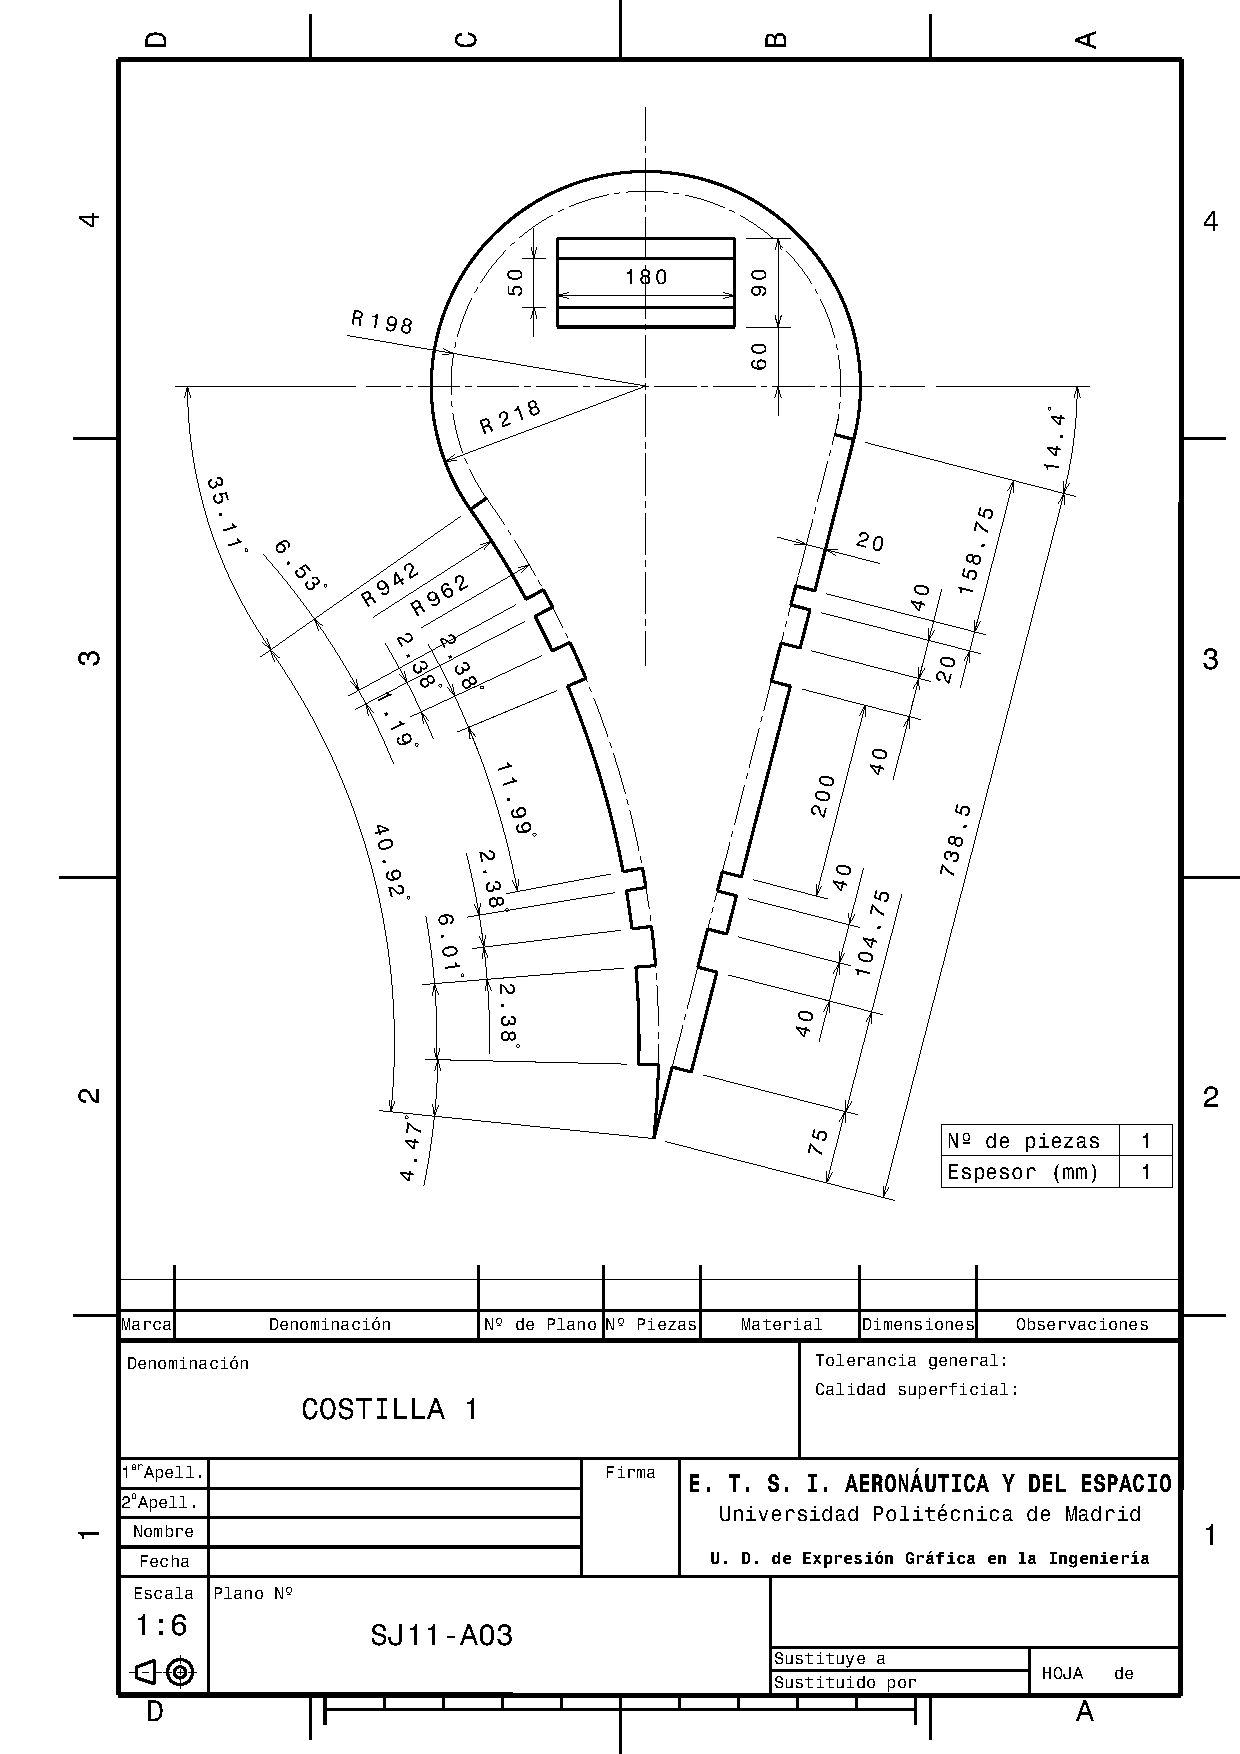
\includegraphics[width=\linewidth]{Figures//Planos/C1.pdf}
\end{figure}

\begin{figure}
    \centering
    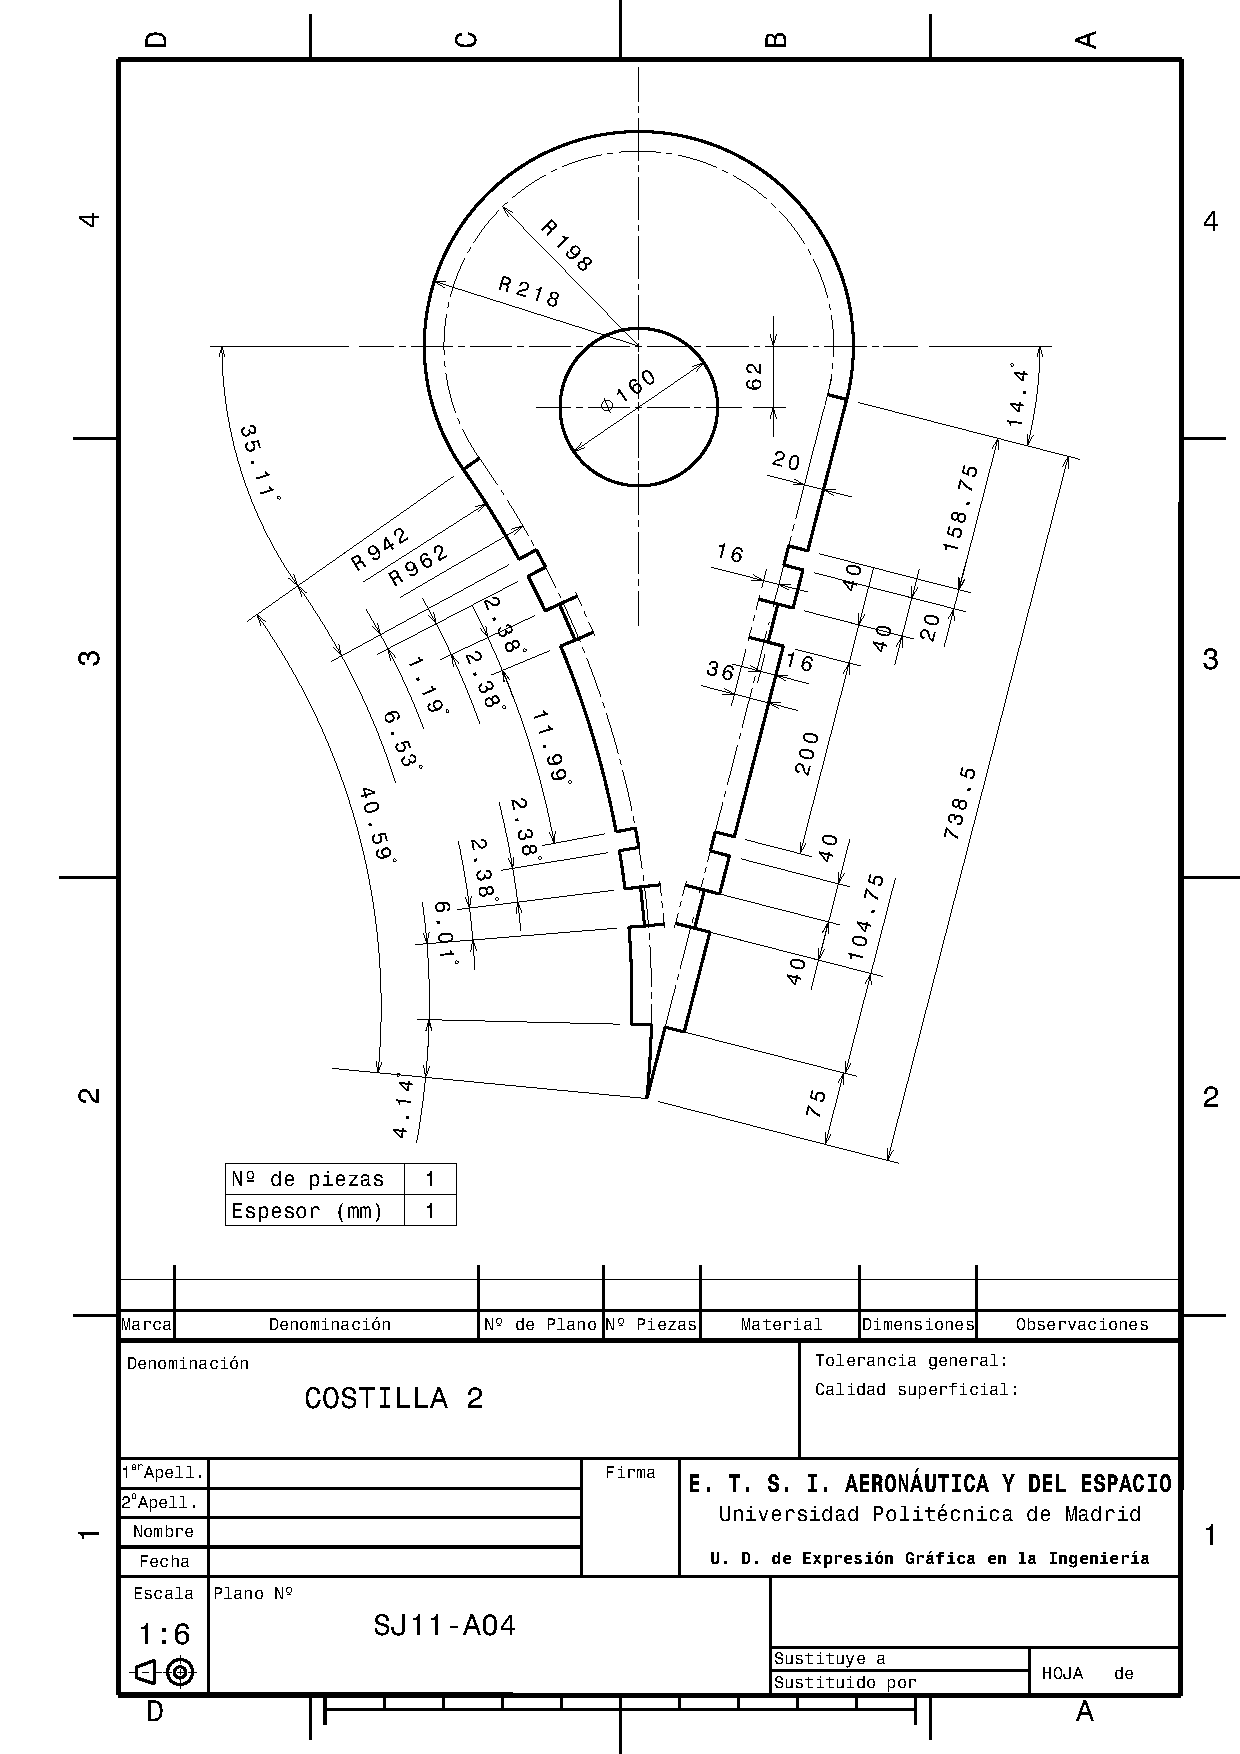
\includegraphics[width=\linewidth]{Figures//Planos/C2.pdf}
\end{figure}

\begin{figure}
    \centering
    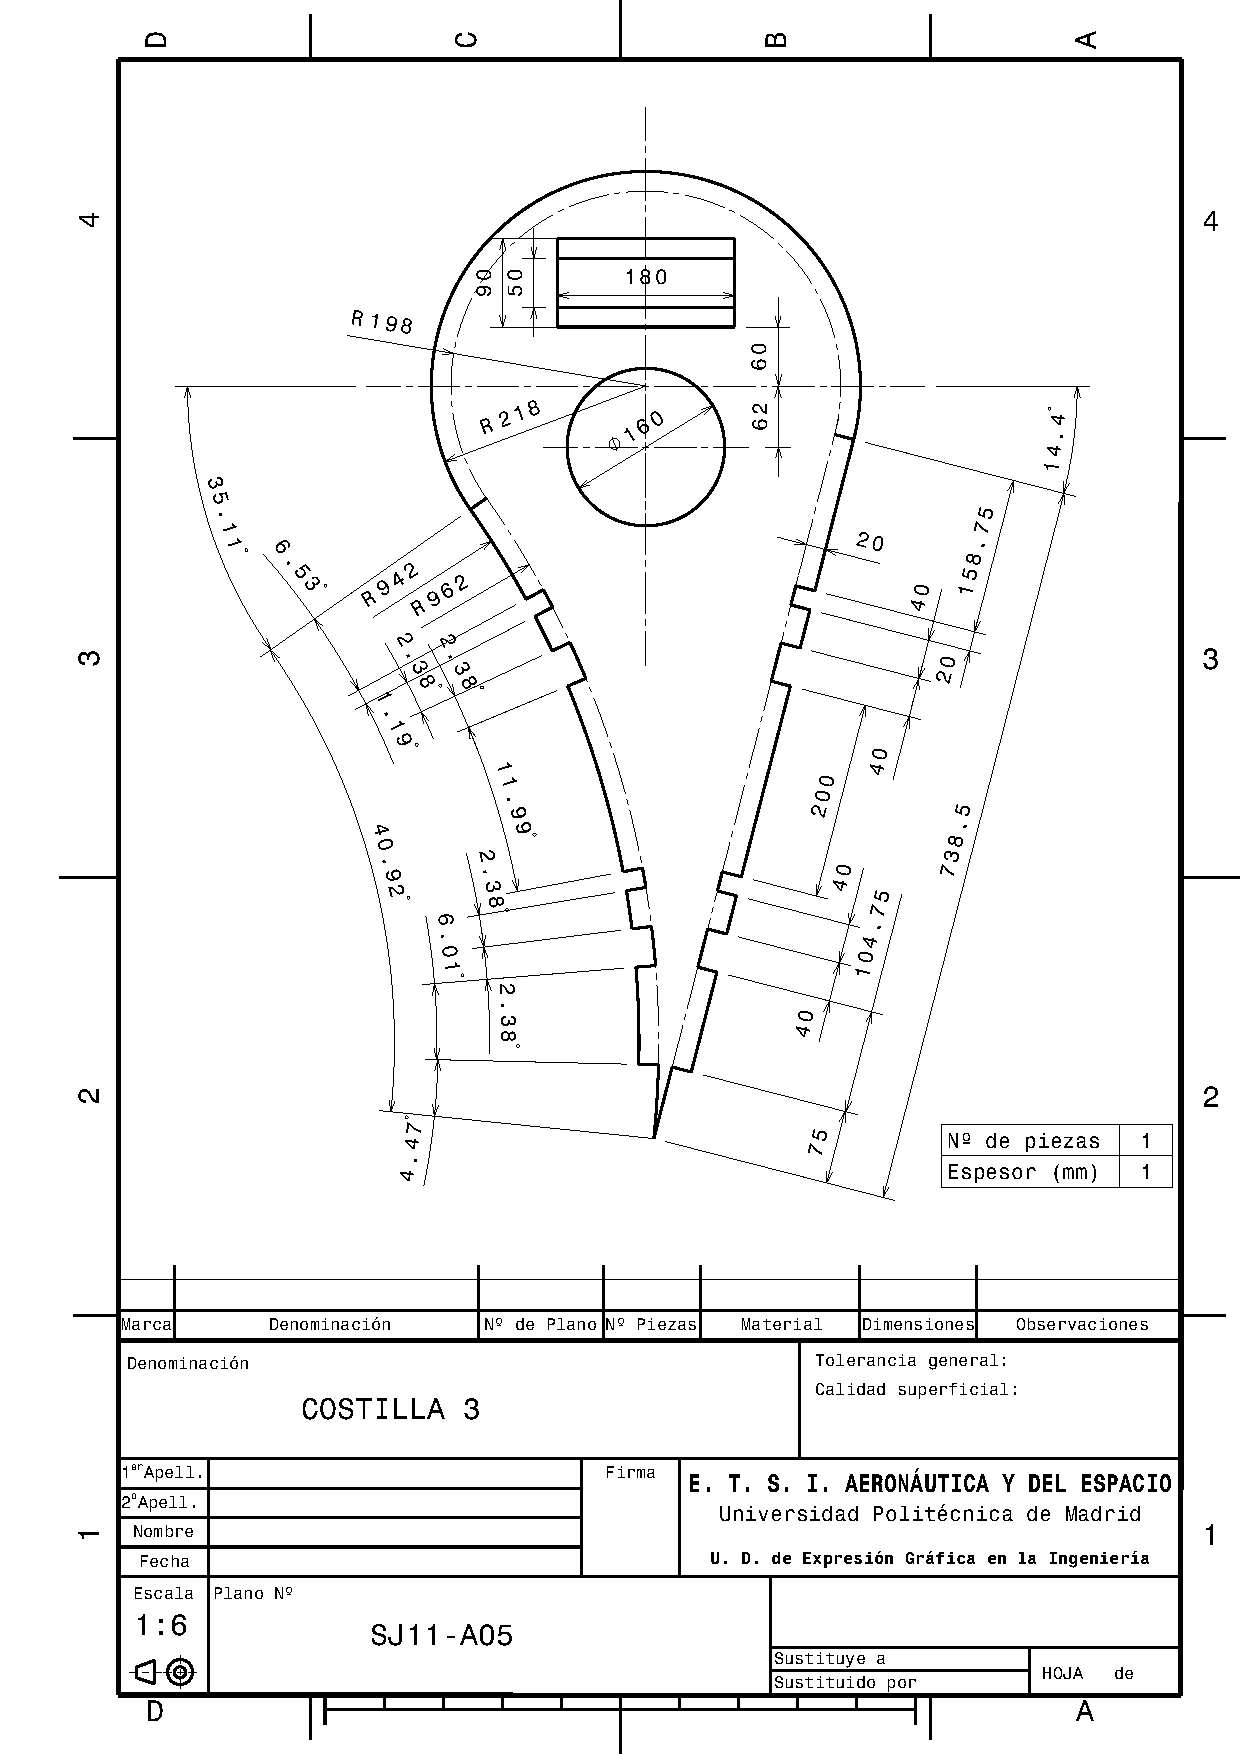
\includegraphics[width=\linewidth]{Figures//Planos/C3.pdf}
\end{figure}

\begin{figure}
    \centering
    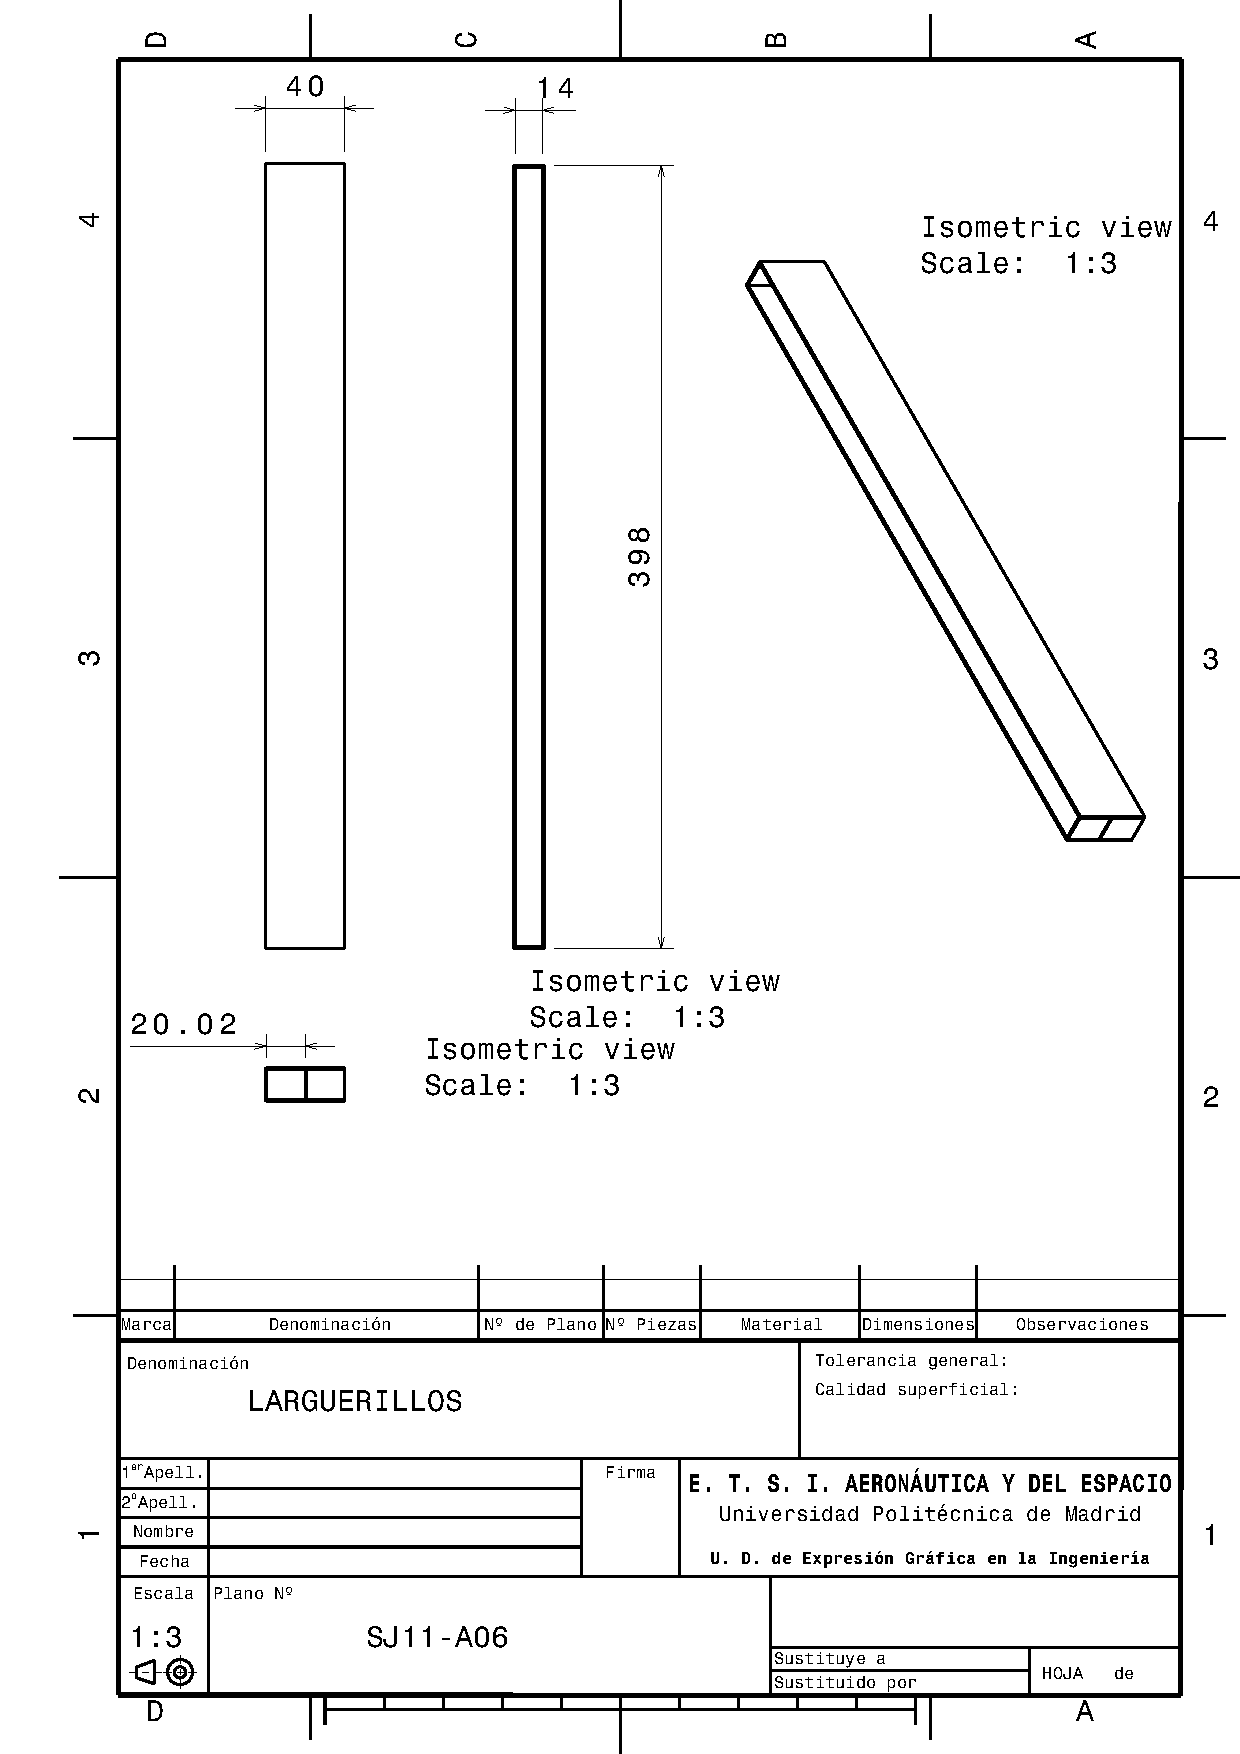
\includegraphics[width=\linewidth]{Figures//Planos/L.pdf}
\end{figure}

\begin{figure}
    \centering
    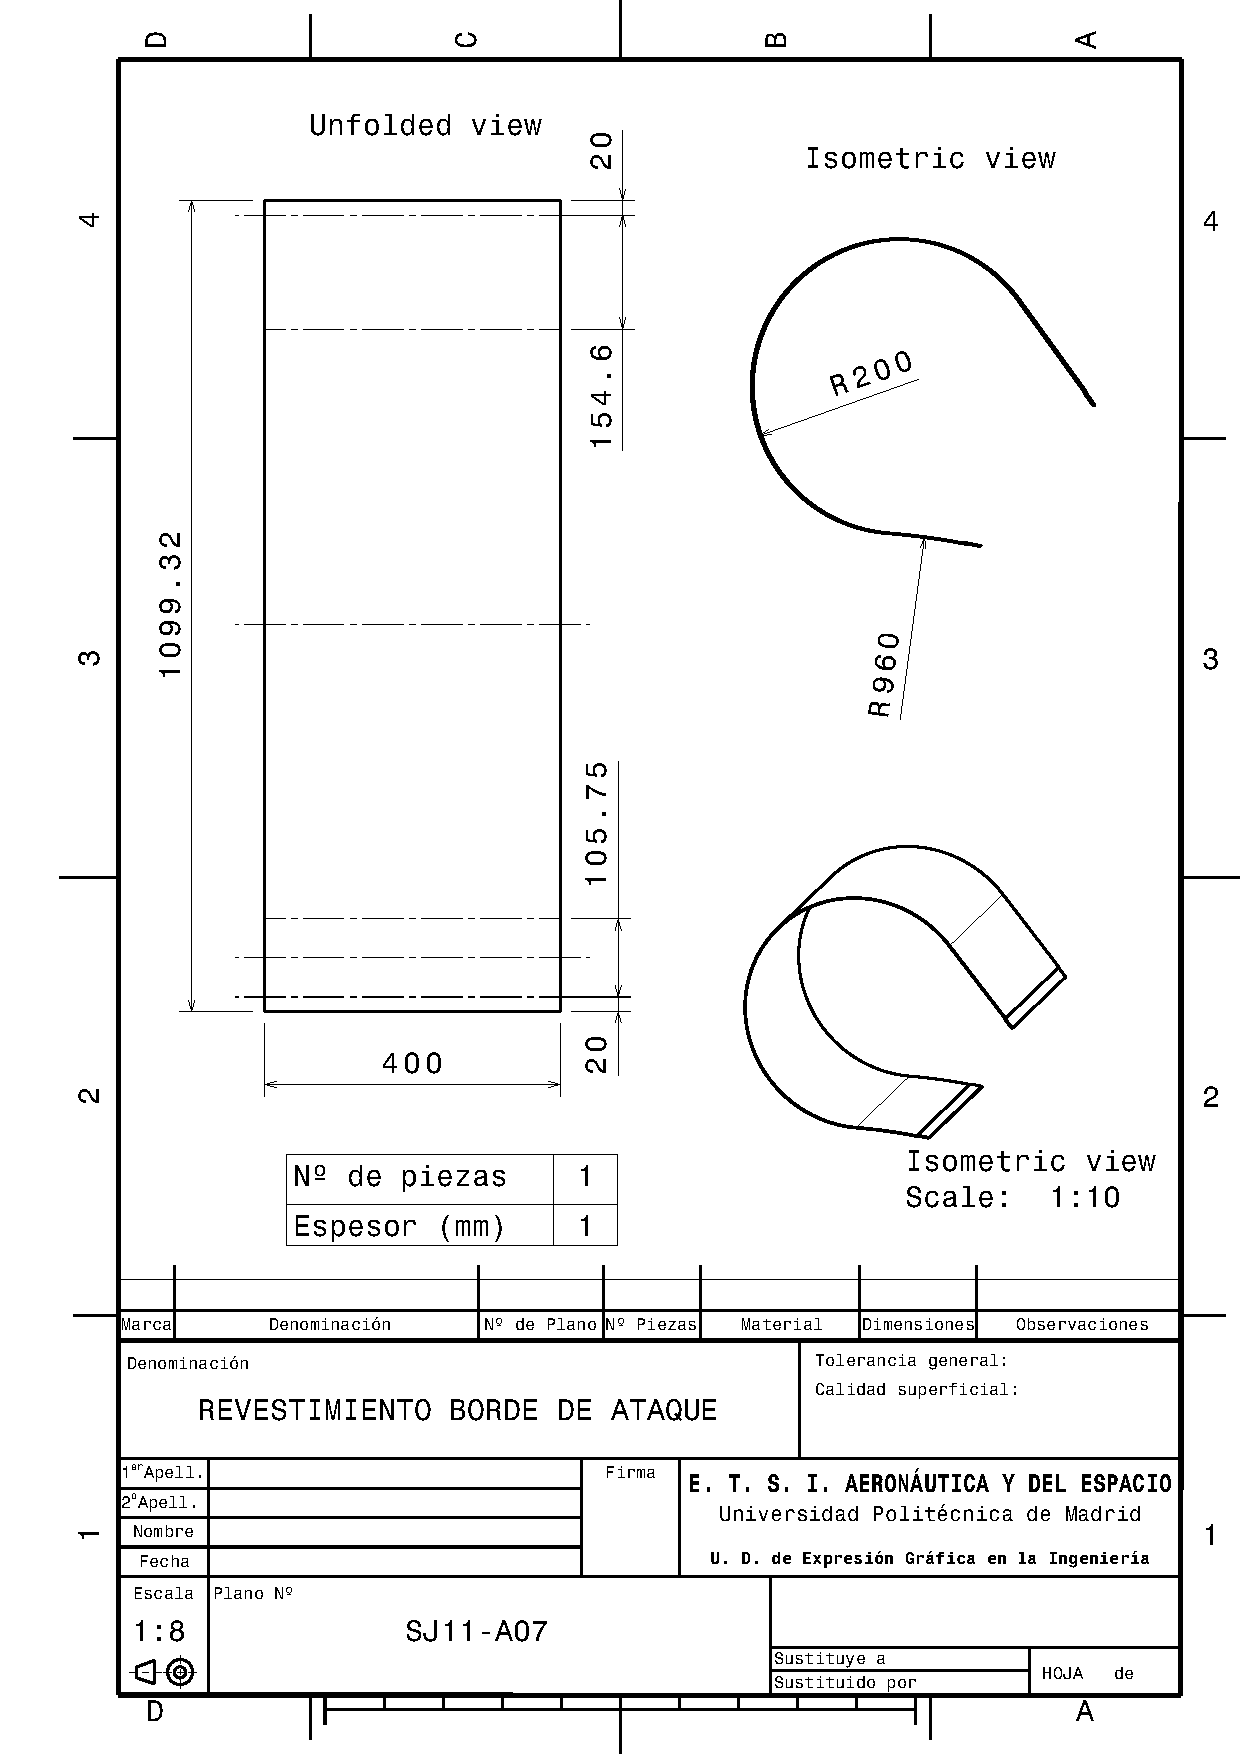
\includegraphics[width=\linewidth]{Figures//Planos/RBA.pdf}
\end{figure}

\begin{figure}
    \centering
    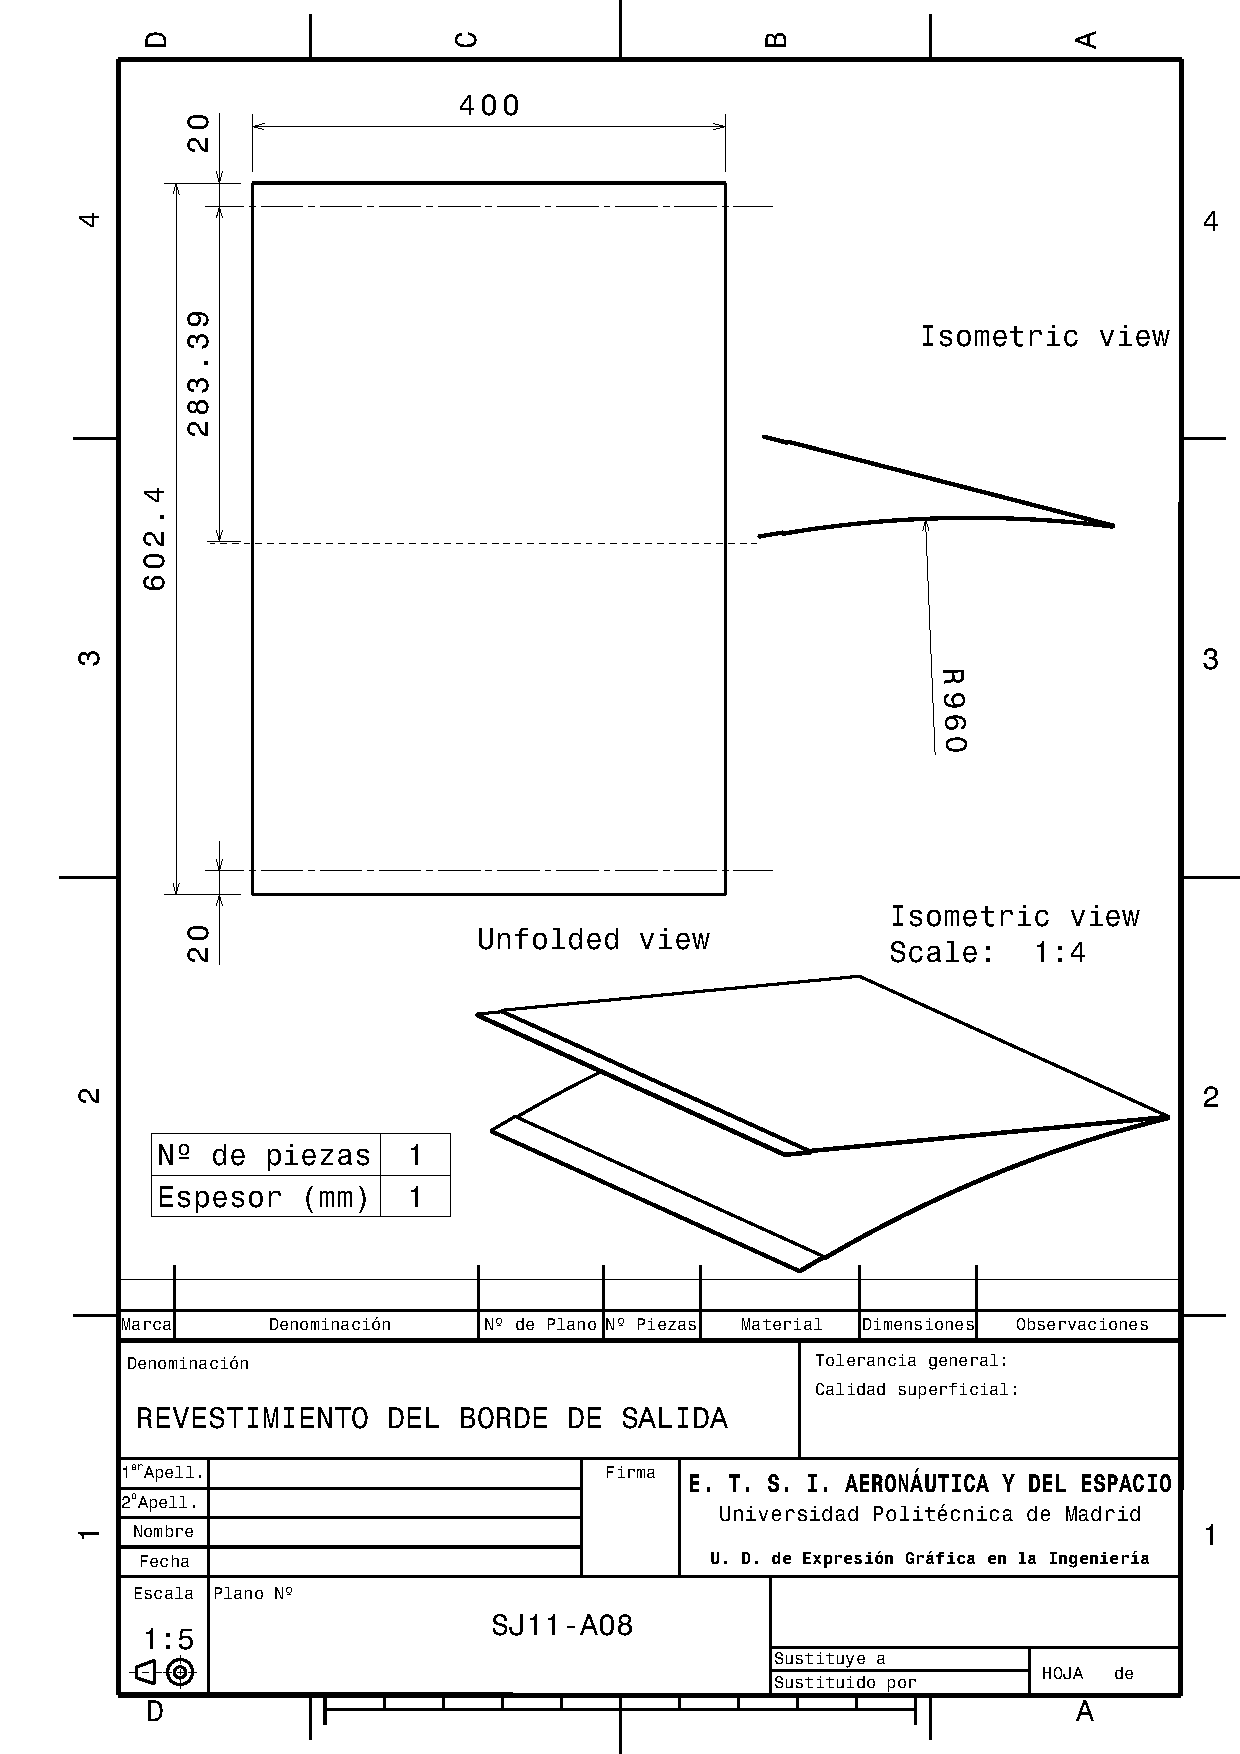
\includegraphics[width=\linewidth]{Figures//Planos/RBS.pdf}
\end{figure}

\begin{figure}
    \centering
    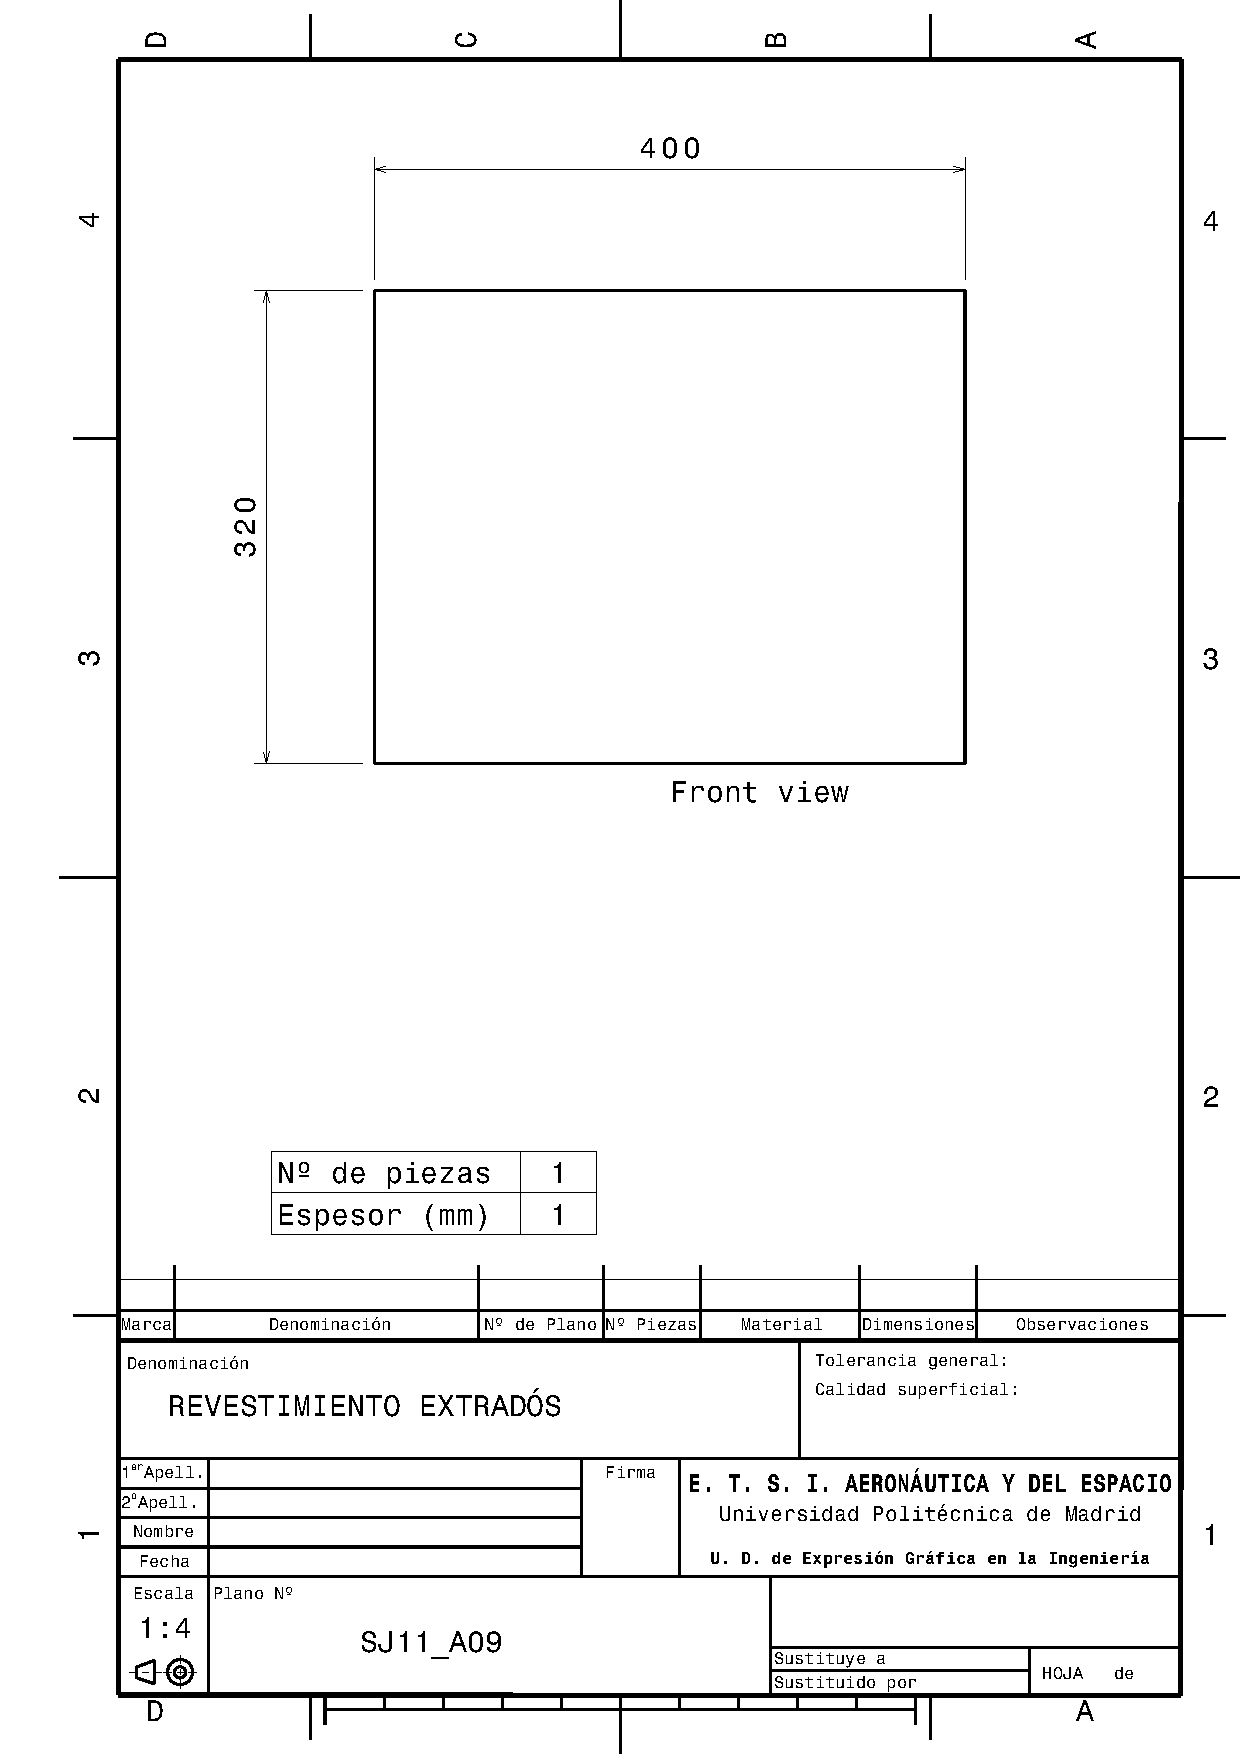
\includegraphics[width=\linewidth]{Figures//Planos/REX.pdf}
\end{figure}

\begin{figure}
    \centering
    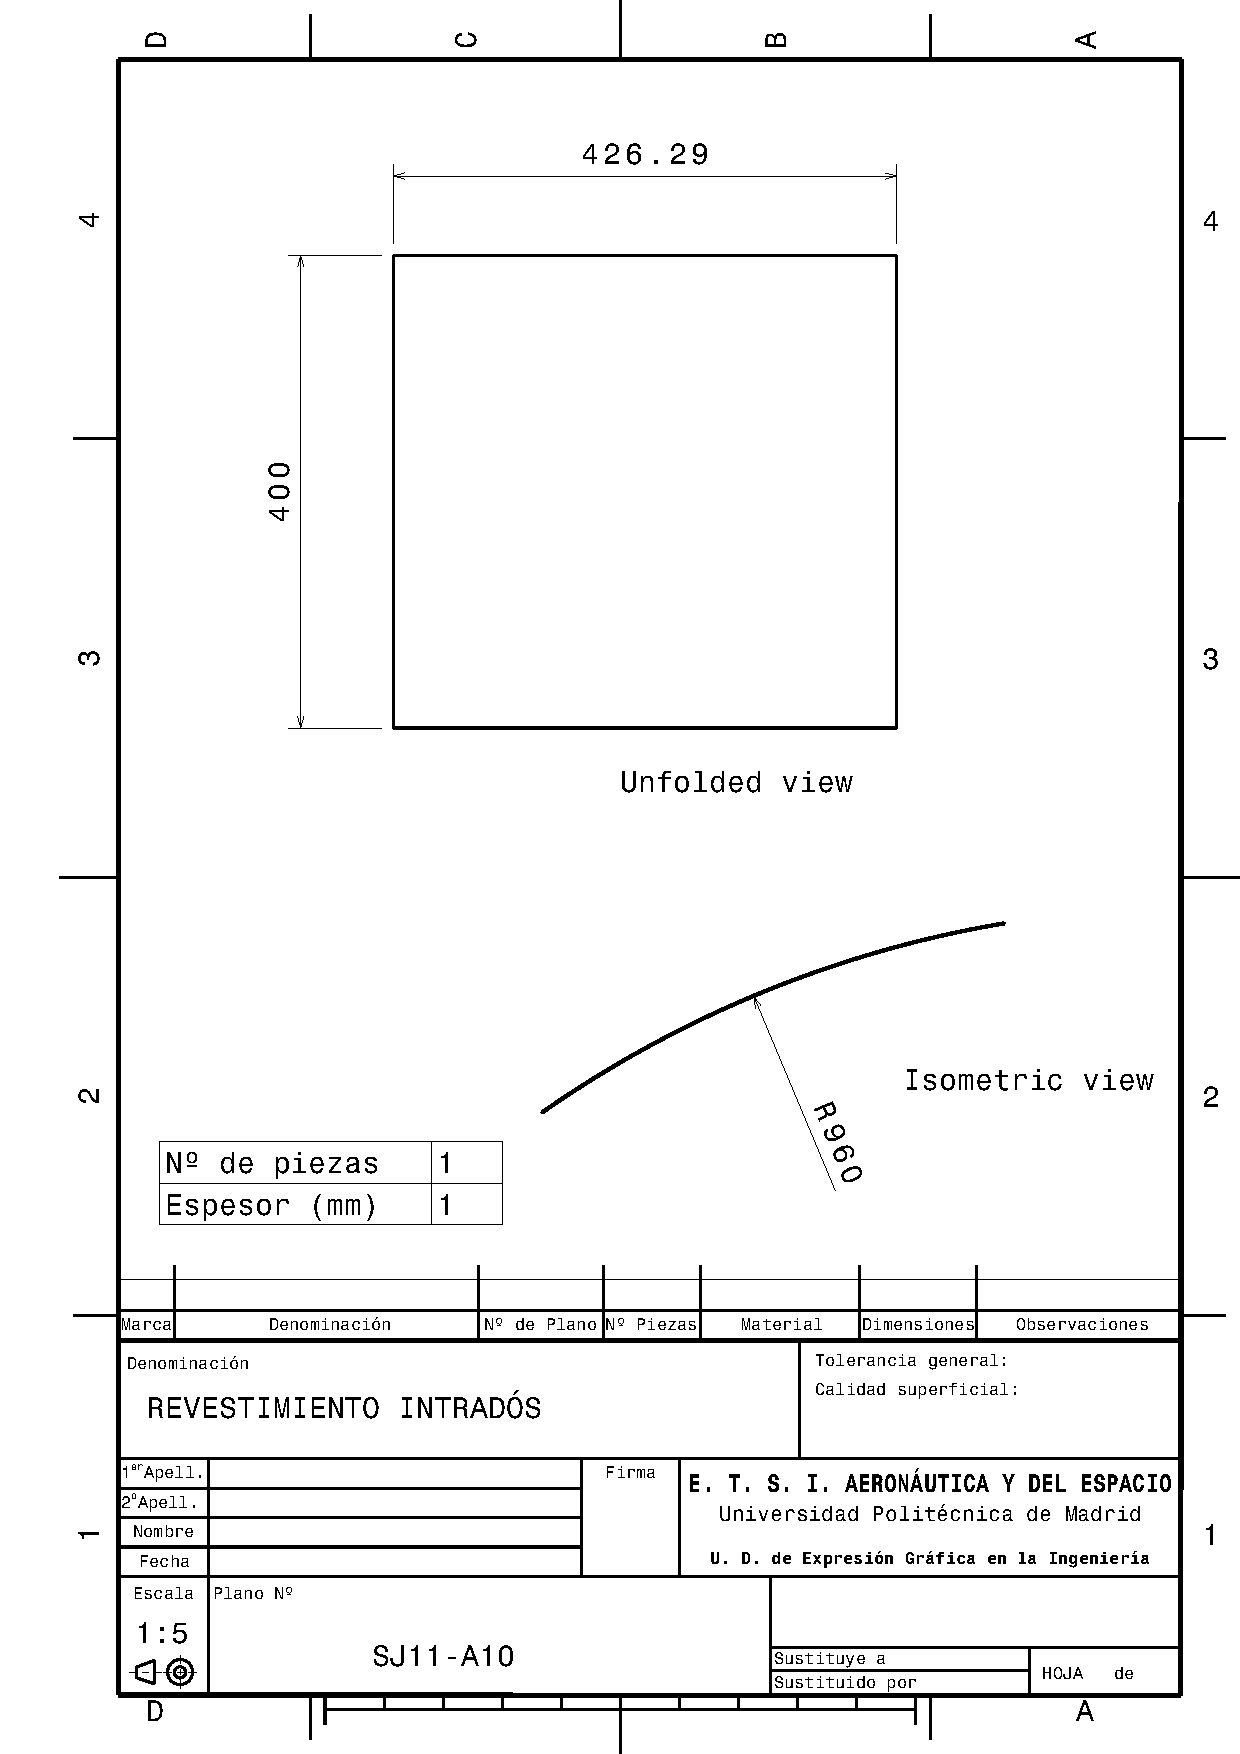
\includegraphics[width=\linewidth]{Figures//Planos/RINT.pdf}
\end{figure}

\begin{figure}
    \centering
    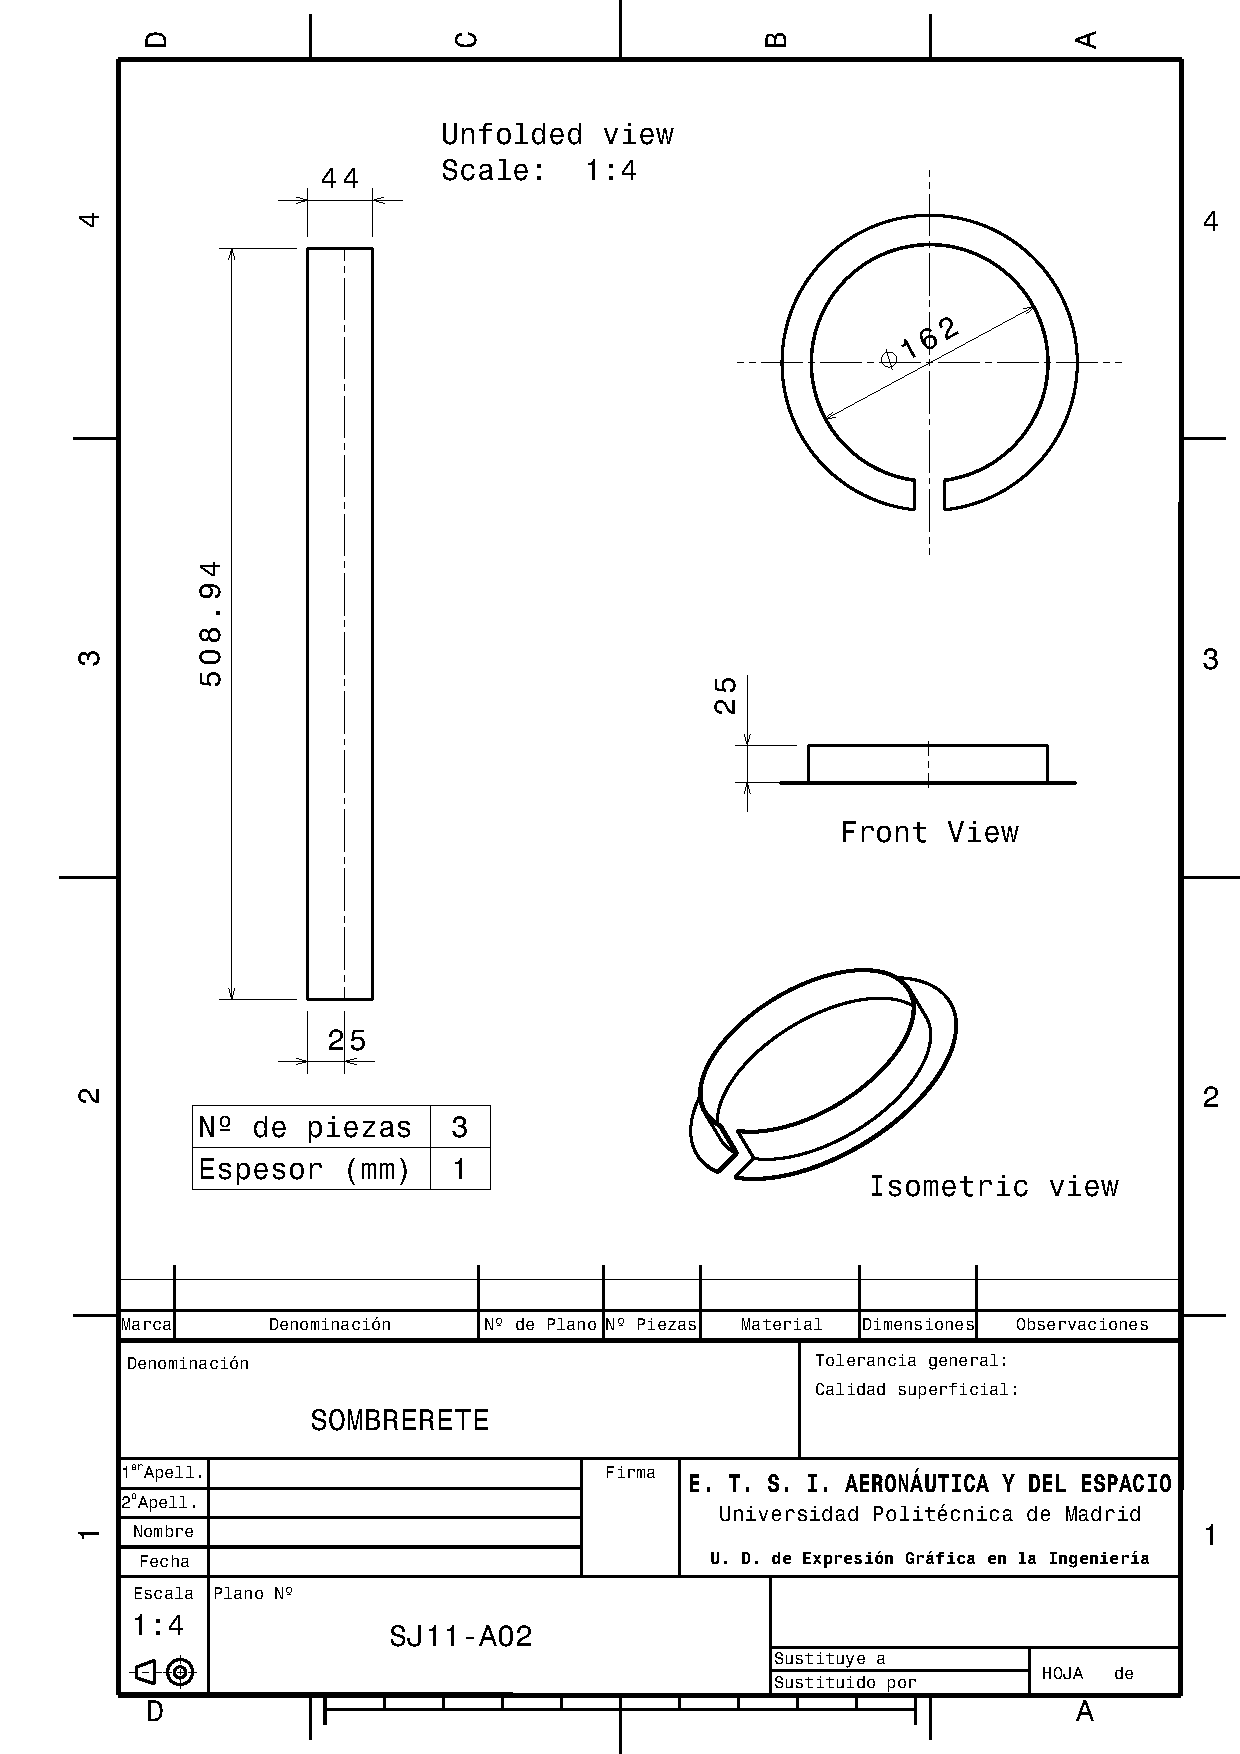
\includegraphics[width=\linewidth]{Figures//Planos/S.pdf}
\end{figure}

\begin{figure}
    \centering
    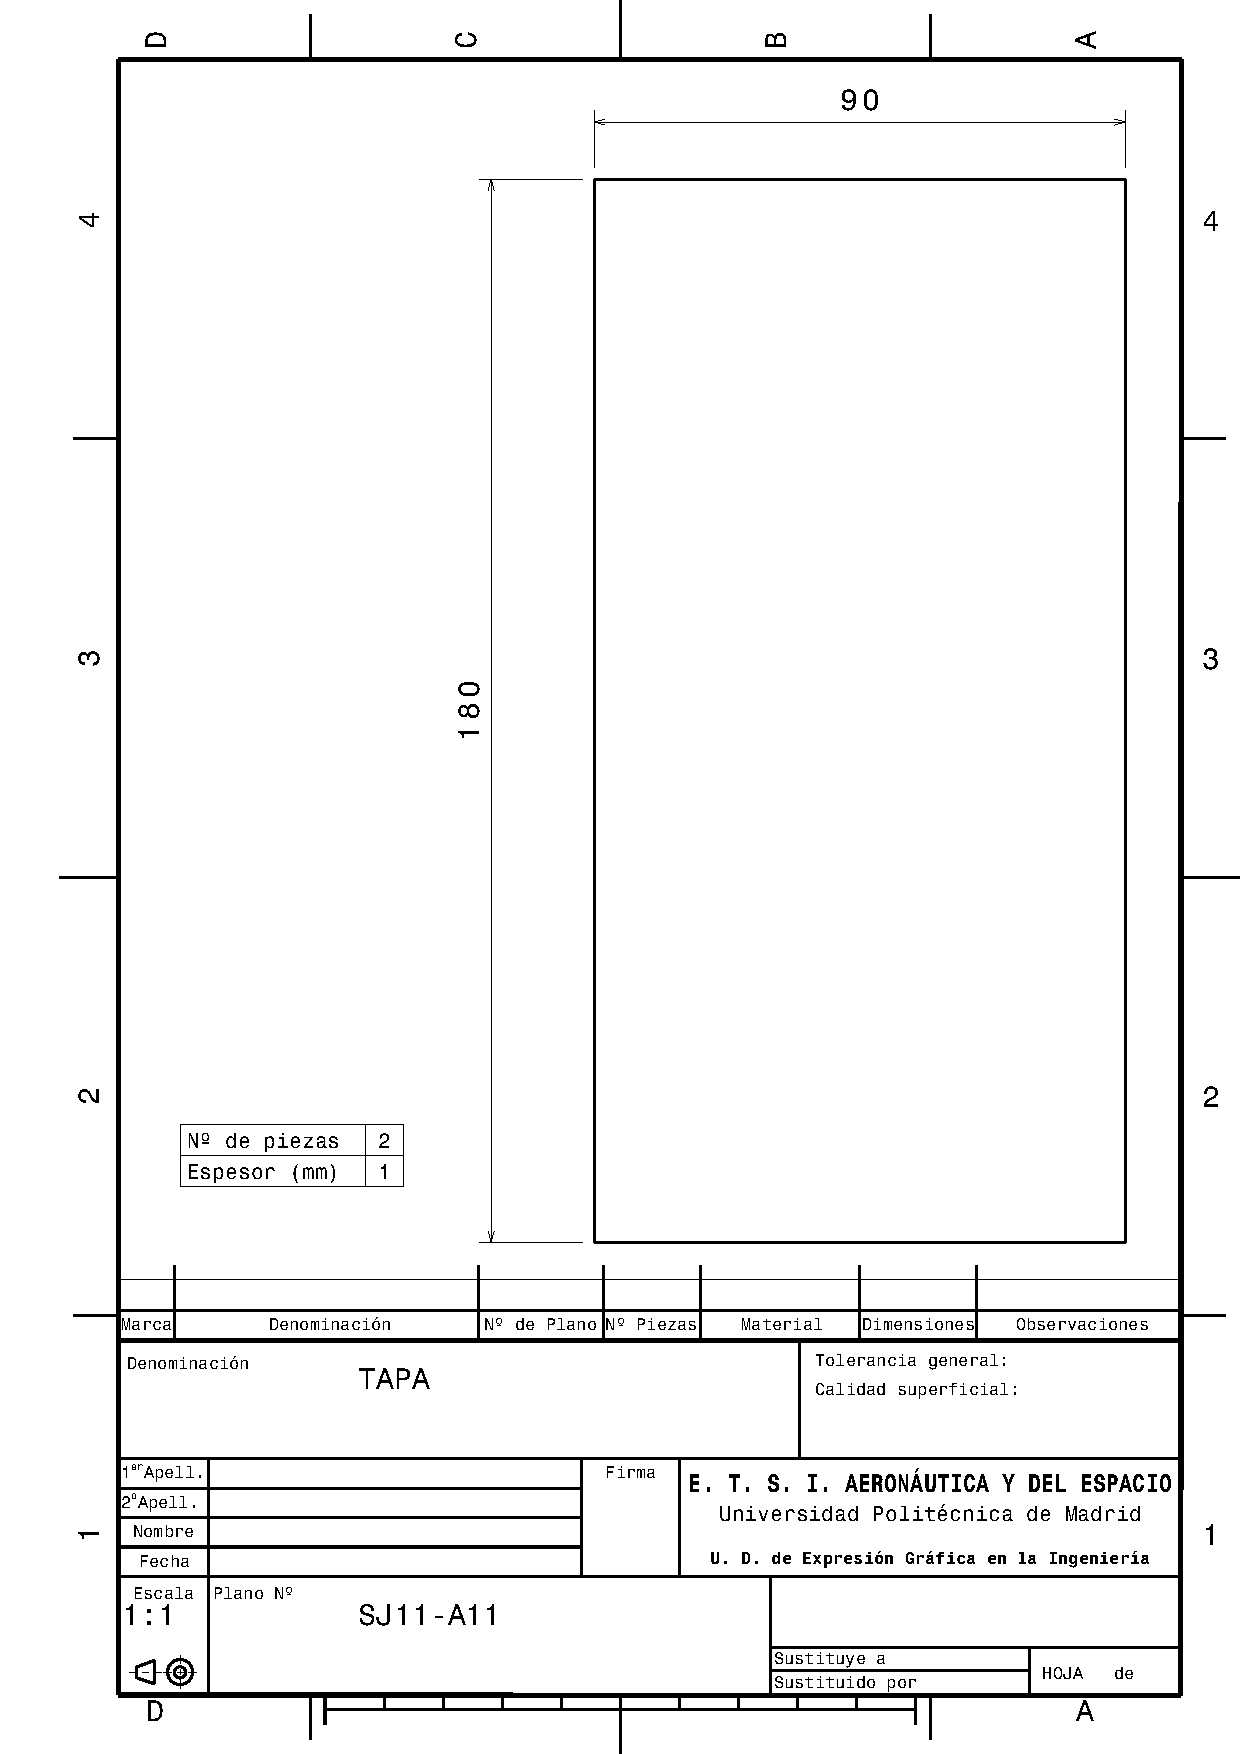
\includegraphics[width=\linewidth]{Figures//Planos/TAP.pdf}
\end{figure}

\begin{figure}
    \centering
    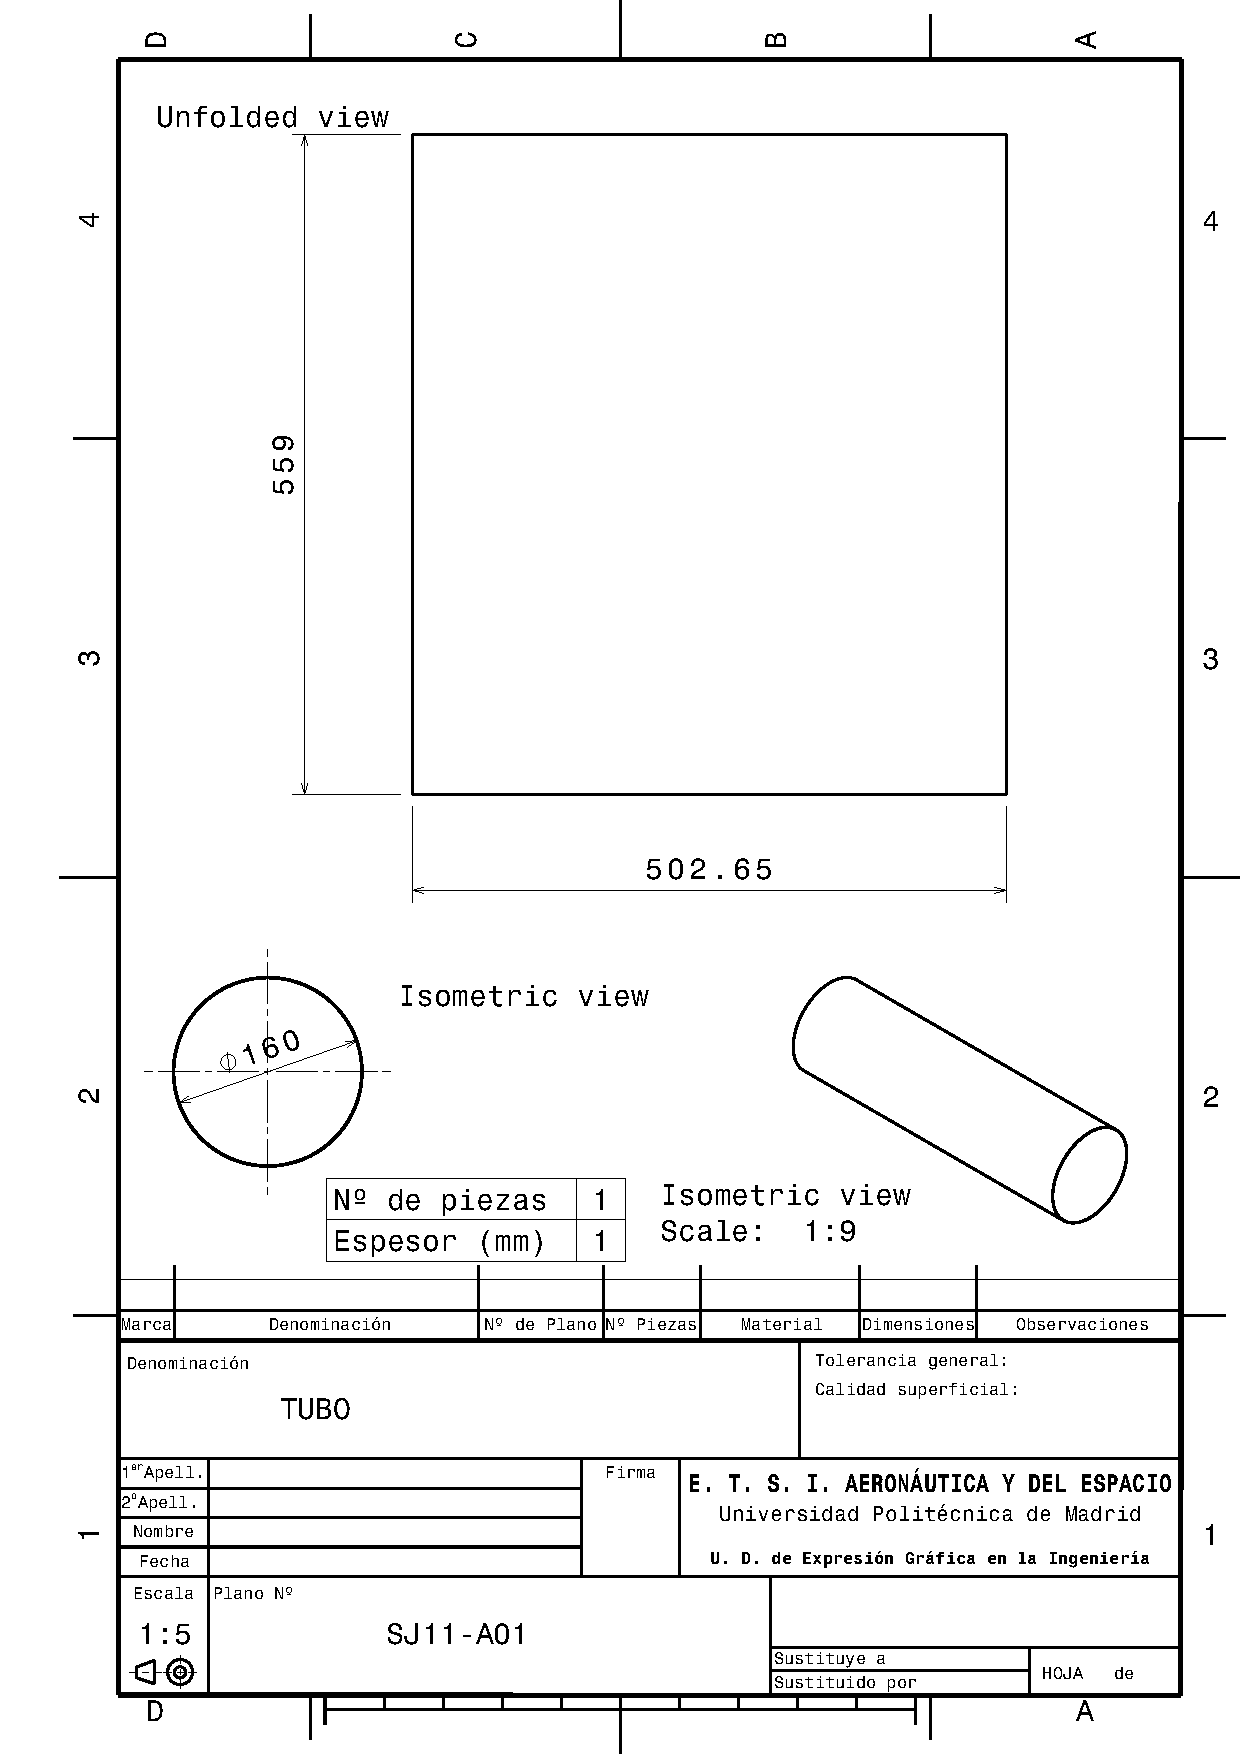
\includegraphics[width=\linewidth]{Figures//Planos/TUB.pdf}
\end{figure}
\cleardoublepage
\chapter{Uniones}

\section{Elección del Método de Unión}
El Perfil se fabricará en acero, por tanto se nos presentan dos vías posibles para realizar la unión:
\begin{itemize}
    \item Soldadura. Bien sea por puntos o la oxiacetilénica.
    \item Remachado.
\end{itemize}

En general, la elección del método de unión dependerá de consideraciones sobre la eficiencia, costo y otros factores. En este caso, al ser un perfil aerodinámico, necesitamos evitar a toda costa cualquier tipo de deformación, pues estas, por pequeñas que sean, podrían afectar a la aerodinámica e invalidar el ensayo. Por ende, descartamos la soldadura, que genera deformaciones inherentemente, en favor del remachado.

\subsection{Elección del Remachado}
La elección del tipo de remachado dependerá de diversos factores: tipo de unión, accesibilidad, ubicación, etc. Según su accesibilidad, se nos presentan dos opciones:
\begin{itemize}
    \item Remaches de caña maciza. Permiten el acceso por ambos lados de la unión, y proporcionan mayor resistencia. 
    \item Remaches ciegos. Tan solo permite el acceso por un lado de la unión.
\end{itemize}

Por tanto, basándonos en lo anterior, elegiremos remaches de cabeza avellanada en zonas con requerimientos aerodinámicos, pero optaremos por remaches de cabeza universal\footnote{También conocidos como de \textit{gota de sebo}.} en zonas sin estos requerimientos, por ser más económicos. Cuando haya accesibilidad por sendos lados, optaremos por usar remaches de caña maciza, por ser más resistentes. En todos los casos, los remaches serán de cabeza normal, lo que asegura tanto la calidad como la funcionalidad de las uniones.

\section{Cálculo de los Remaches}

Basándonos en la normativa aplicable, para un remache de cabeza de cierre normal, se usan las siguientes expresiones:
\begin{gather}
    l = e + 1.5d, \\
    D = 1.5d, \\
    K = 0.4d,
\end{gather}

donde $l$ es la longitud de la caña, $d,$ el diámetro del remache, $D$ el diámetro de la cabeza de cierre, y $K$ la longitud de la cabeza del remache (ver figura \ref{fig:remaches}).
\begin{figure}[!htb]
    \centering
    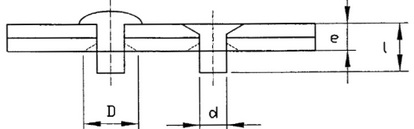
\includegraphics[width=0.5\linewidth]{Figures/remaches.png}
    \caption{Representación de medidas de un remache de cabeza normal y de un remache avellanado}
    \label{fig:remaches}
\end{figure}

En el caso de remaches con cabeza avellanada, empleamos:
\begin{gather}
    l = e_T + 0.8d = 5.2 \quad \text{[mm]}, \\
    D = 2d = 8 \quad \text{[mm]}, \\
\end{gather}

siendo $e_T$ el espesor total de la chapas a unir. 

Según \textit{Remaches y Herramientas}\cite{remaches} y considerando acero, $d = 4 \text{[mm]}$ para los remaches, y un espesor de la chapa de $e_{\text{Ac}} = 1 \text{[mm]}$.

Se ha elegido una distancia al borde del remache de $10 \text{[mm]}$, que es $0.5 \text{[mm]}$ más que la distancia mínima recomendada por la normativa:
\begin{equation}
    E \ge 2d + 1.5 = 9.5 \quad \text{[mm]}.
\end{equation}

Respecto a la distancia entre remaches, la normativa marca que debe ser, al menos, cuatro veces el diámetro para remaches (ver figura \ref{fig:dist}):

\begin{equation} \label{eq:p}
    P > 4d = 16 \quad \text{[mm]}.
\end{equation}

\begin{figure}[!htb]
    \centering
    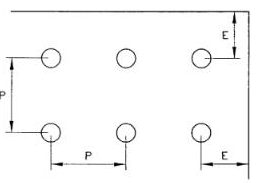
\includegraphics[width=0.3\linewidth]{Figures/distancia.png}
    \caption{Distancia entre remaches}
    \label{fig:dist}
\end{figure}

Las uniones quedan recogidas a continuación\footnote{Cálculos redondeados a la baja}:

\begin{table}[!htb]\centering

\begin{tabular}{|l|r|}\hline
\rowcolor[HTML]{C0C0C0}\textbf{Línea de Unión} 
& \textbf{Tipo de Soldadura}\\\hline
Sombreretes - Tubo & Soldadura oxiacetilénica \\\hline
Larguerillo - Costilla & Soldadura por puntos \\\hline
\end{tabular}
\end{table}

\begin{landscape}
    \vspace*{\fill}
    \begin{table}[H]\centering

\begin{tabular}{|l|r|r|r|}\hline
\rowcolor[HTML]{C0C0C0}\textbf{Línea de Unión} &\textbf{Tipo de Caña} &\textbf{Cabeza} &\textbf{Longitud \tablefootnote{Longitud sin Deformar} [mm]} \\\hline
Unión Sombrerete - Costilla &Caña maciza &Universal &8 \\\hline
Revestimiento borde de ataque – Costilla ($\times 3$) &Ciego y caña maciza &Universal &8 \\\hline
Zona plana revestimiento del borde de salida ($\times 3$) &Ciego &Avellanada \tablefootnote{Zona con función aerodinámica, por tanto se ha de usar remachado avellanado. Se calcula usando cabezas de tipo universal para facilitar los cálculos. \label{av}}  &8 \\\hline
Zona curva revestimiento del borde de salida ($\times 3$) &Ciego &Avellanada \footref{av}  &8 \\\hline
Revestimiento borde de ataque – Revestimiento extradós  ($\times 3$) &Caña maciza &Avellanada &8 \\\hline
Revestimiento borde de ataque – Revestimiento intradós ($\times 3$) &Ciego &Avellanada \footref{av} &8 \\\hline
Revestimiento borde de salida – Revestimiento intradós  ($\times 3$)&Ciego &Avellanada \footref{av} &8 \\\hline
Revestimiento extradós ($\times 3$)&Caña maciza &Avellanada \footref{av} &8 \\\hline
Revestimiento intradós  ($\times 3$) &Caña maciza &Avellanada &8 \\\hline
Revestimiento borde de salida – Revestimiento extradós  ($\times 3$) &Caña maciza &Avellanada \footref{av} &8 \\\hline
Larguerillo delantero – Revestimiento intradós &Ciego &Avellanada \footref{av} &8 \\\hline
Larguerillo delantero – Revestimiento extradós &Caña maciza &Avellanada \footref{av} &8 \\\hline
Larguerillo trasero – Revestimiento borde de salida &Ciego &Avellanada \footref{av} &8 \\\hline
Tapa acceso - Costilla exterior ($\times 2$) &Caña maciza &Avellanado &8 \\ \hline
\end{tabular}
\end{table}
    \vspace*{\fill}
    \clearpage
\end{landscape}

\subsection{Cálculos Uniones}
\subsubsection{Unión Sombretes - Costillas}
Empleamos remaches de caña maciza y cabeza normal (por cuestión de accesibilidad) equiespaciados entre sí 17 [mm], superior a la distancia dada por la ecuación \ref{eq:p}. El remachado se hace a lo largo de la línea media. Al existir tres costillas con un sombrerete cada una, necesitaremos un total de 96 remaches.

\begin{equation}
    L_s = 2\pi \bigg( \dfrac{200-162}{2} + \dfrac{162}{2} \bigg) = 568.63 \quad \text{[mm]}.
\end{equation}

Al haber un acceso, tendremos que restar 20 [mm] al perímetro de la línea media:
\begin{equation}
    L_{s,\, \text{real}} = 548.63 \quad \text{[mm]}.
\end{equation}

El número de remaches se calcula como:
\begin{equation}
    N = \dfrac{548.63}{17} = 32.27 \approx 32 \quad \text{[Remaches]} \times \text{Costilla}.
\end{equation}

La distancia real es:
\begin{equation}
    P_{\text{real}} = \dfrac{548.63}{32} = 17.15 \quad \text{[mm]}
\end{equation}

\subsubsection{Revestimiento Borde de Ataque - Costillas} \label{subsub:ba}
Vamos a necesitar taladrar los puntos donde se vayan a utilizar remaches. El bordonado no se taladrará ni remachará aún\footnote{Se hará cuando se instalen los revestimientos del extradós e intradós, para asegurar la alineación}, pero se tendrá en cuenta para el cálculo. Estos agujeros atravesarán los dos revestimientos y la costilla sin presentar desviaciones.

Todos los remaches se situarán en la línea media de la solapa, y se tendrá en cuenta 9.5 [mm] de espaciado hasta los bordes.

Unión de revestimiento del borde de ataque - costillas:
\begin{equation}
    L_r = 1099.32 \quad \text{[mm]}.
\end{equation}

Longitud real del remachadao, teniendo en cuenta los espaciados desde los bordes:
\begin{equation}
    L_{\text{real}} = 1099.32 - 2 \cdot 10 = 1079.32 \quad \text{[mm]}.
\end{equation}

Número de remaches:
\begin{equation}
    N = \dfrac{1079.32}{17} = 63.49 \approx 63 \quad \text{Remaches} \times \text{Costilla}.
\end{equation}

\begin{equation}
    P_{\text{real}} = \dfrac{1079.32}{63} = 17.13 \quad \text{[mm]}
\end{equation}

Dejaremos los remaches de los bordes sin remachar, por tanto, el número de remaches utilizados serán 2 menos por costilla, por lo que habrá un total de 183 remaches hasta el bordonado.

\subsubsection{Unión Larguerillos - Costillas}
Se debe proceder con cuidado para asegurar una unión adecuada sin comprometer la integridad estructural o la aerodinámica de la pieza. Usaremos la soldadura por puntos, empleando un equipo de soldadura por resistencia, que es muy efectiva para reducir la deformación del material, puesto que el calor se concentra solo en los puntos de soldadura, reduciendo el efecto térmico.

\subsubsection{Revestimiento Borde de Salida - Costillas} \label{subsub:bs}
Mismo procedimiento que el explicado en \ref{subsub:ba}. Los remaches se colocan en la línea media de la solapa de las costillas en contacto con el revestimiento, dejando un espaciado de 10 [mm] a los bordes.

Unión revestimiento:
\begin{equation}
    L_r = 602.4 \quad \text{[mm]}.
\end{equation}

Longitud real del remachado:
\begin{equation}
    L_{\text{real}} = 602.4 - 2 \times 10 = 584.4 \quad \text{[mm]}.
\end{equation}

Número de remaches:
\begin{equation}
    N = \dfrac{584.4}{17} = 34.38 \approx 34 \quad \text{Remaches} \times \text{Costilla}.
\end{equation}

\begin{equation}
    P_{\text{real}} = \dfrac{584.4}{34} = 17.19 \quad \text{[mm]}
\end{equation}

Al igual que pasaba en \ref{subsub:ba}, el número de remaches es 2 menos por costilla. Es decir, hay un total de 102 remaches hasta el bordonado.

\subsubsection{Revestimiento Borde de Ataque - Revestimiento Extra e Intradós} \label{subsub:rba}
En el primer bordonado comienza el revestimiento del extradós e intradós, por lo que habrá un remache justo en el centro del bordonado, dejando 10 [mm] hasta el borde. Es decir, habrá que poner los remaches que no hemos puesto en \ref{subsub:ba}.


\subsubsection{Revestimiento Borde de Salida - Revestimiento Extra e Intradós}
Procedemos análogamente a \ref{subsub:rba}. Teniendo en cuenta lo expuesto en \ref{subsub:bs}, tendremos que colocar los 6 remaches que no pusimos entonces.

\subsubsection{Larguerillos - Revestimiento Extradós e Intadós}
Por cada larguerillo habrá dos hileras de remaches separadas entre sí por 20 [mm] y que se sitúan entre las dos costillas exteriores\footnote{Recordemos que estarán unidas por soldadura por punto}. Las dos hileras se encargan de unir el revestimiento en cuestión al larguerillo. 

Como la longitud entre costillas es de 400 [mm]:
\begin{equation}
    L_r = (400 - 4 \cdot 10) = 360 \quad \text{[mm] $\times$ larguerillo}.
\end{equation}

Número de remaches:
\begin{equation}
    N = \dfrac{360}{17} = 21.18 \approx 21 \quad \text{Remaches}.
\end{equation}

\begin{equation}
    P_{\text{real}} = \dfrac{360}{21} = 17.14 \quad \text{[mm]}.
\end{equation}

\subsubsection{Tapa de Acceso - Solapes de Acceso - Costilla}
La costilla proporciona dos solapes a cada lado del acceso, que van unidos a la propia costilla mediante una hilera de remaches. Posteriormente, al otro lado del solape que sobrasale 20 [mm] en la apertura de acceso, se remachará en la línea media con la tapa, dejando, para ambos casos, 10 [mm] en los bordes\footnote{Cumple lo establecido en la normativa, 9.5 [mm]}, ya que el solape mide 40 [mm].

\begin{equation}
    L_r = 180 - 2 \cdot 10 = 160 \quad \text{[mm]}.
\end{equation}

Número de remaches:
\begin{equation}
    N = \dfrac{160}{17} = 9.41 \approx 9 \quad \text{Remaches $\times$ Hilera}.
\end{equation}

Espaciado entre remaches:
\begin{equation}
    P_{\text{real}} = \dfrac{160}{9} = 177.78 \quad \text{[mm]}.
\end{equation}

\subsubsection{Revestimiento Intradós - Costilla}

\begin{equation}
    L_r = 426.29 - 2 \cdot 10 = 406.29 \quad \text{[mm]}.
\end{equation}

Número de remaches:
\begin{equation}
    N = \dfrac{406.29}{17} = 23.90 \approx 23 \quad \text{Remaches $\times$ Costilla}.
\end{equation}

Espaciado entre remaches:
\begin{equation}
    P_{\text{real}} = \dfrac{406.29}{23} = 17.66 \quad \text{[mm]}.
\end{equation}

\subsubsection{Revestimiento Extradós - Costilla}
\begin{equation}
    L_r = 320 - 2 \times 10 = 300 \quad \text{[mm]} 
\end{equation}

Número de remaches:
\begin{equation}
    N = \dfrac{300}{17} = 17.65 \approx 17 \quad \text{Remaches $\times$ Costilla}.
\end{equation}

Espaciado entre remaches:
\begin{equation}
    P_{\text{real}} = \dfrac{300}{17} = 17.65 \quad \text{[mm]}
\end{equation}

\subsubsection{Soldadura Tubo - Sombreretes}
Decidimos soldar el tubo y los sombreretes mediante soldadura oxiacetilénica. Al fundirse el límite entre ambas piezas, no se discernirá que son piezas diferentes.

Los Autores aclaramos que, a pesar de que sí que habrá una zona afectada por el calor (i.e. con deformación), no afectará a la aerodinámica.
\cleardoublepage
\chapter{Montaje y Ensamblado}
En todo el proceso de montaje, deberemos de ser extremadamente cautelosos, a fin de evitar errores de unión que comprometerán la integridad estructural o la aerodinámica, echando a perder el perfil.

Antes del montaje al que vamos a proceder, todos los elementos han pasado por un proceso de corte y conformado, donde se han empleado herramientas adecuadas, de calidad y con operarios capacitados.

\section{Proceso}

\subsection{Paso Previo: Preparación de las Costillas en Forma de Perfil Aerodinámico}
Dos de las tres costillas (trasera y delantera) contarán con perforaciones para permitir que la estructura sea accesibles. Para esto, realizamos una perforación rectangular (ancho por alto: $50\times180 \, [\text{mm}]$) en dichas costillas.

Por otro lado, la costilla intermedia y la delantera cuentan con un orificio circular de radio 80 [mm], para poder introducir por su interior el tubo de soporte, que sostendrá a toda la estructura.

Todas las costillas contarán con bordones, sobre los que se apoyarán los larguerillos delanteros y traseros, colocados dos a dos sobre el intradós y el extradós, separados entre sí 260 [mm], y con longitud y profundidad de 40 [mm] y 14 [mm], respectivamente.

Por último, también hay bordones de longitud 20 [mm] para el revestimiento.

\subsection{Primer Paso: Tubo de Soporte}
El tubo de soporte facilita la orientación y sustenta la estructura. Para esto, curvaremos una chapa, obteniendo un tubo de 80 [mm].

Posteriormente, trazamos una generatriz sobre el tubo, donde marcaremos la separación de las costillas (400 [mm]), desde el extremo delantero hacia delante.

Ver figura \ref{fig:primer}.

%===============================================================================================================
%                                                   PRIMER PASO
%===============================================================================================================
\begin{figure}[!htb]
\centering
\begin{tikzpicture}[lablum/.style 2 args={label=below:#1 #2,name=img-#1},
marr/.style={line width=1mm,-latex}]
 \matrix[column sep=1cm,row sep=5mm] (mat)
 { \node[lablum={a}{}]{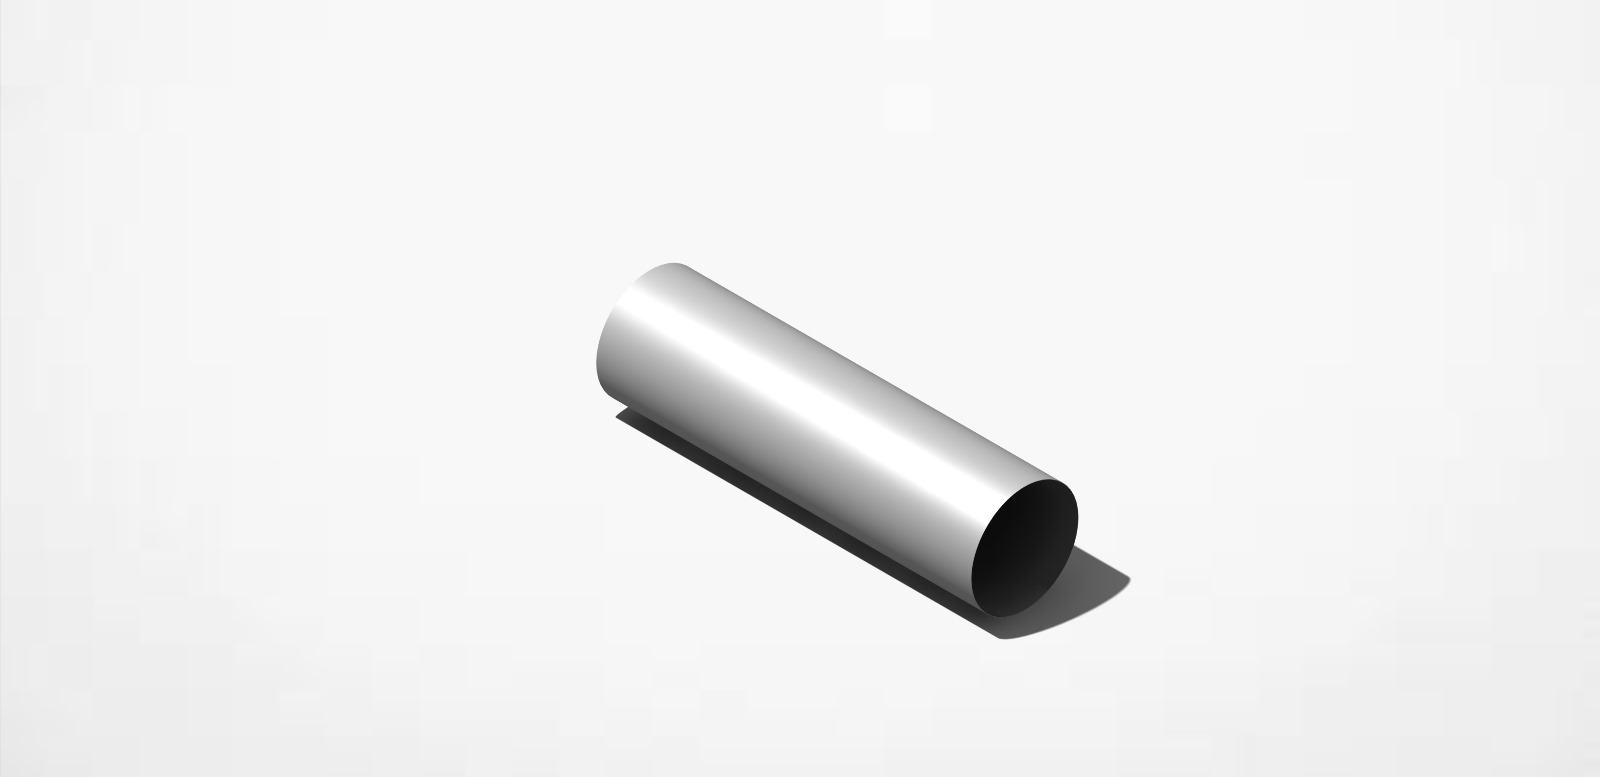
\includegraphics[width=5.5cm]{Figures/Montaje/1.jpg}};
 & \node[lablum={b}{}]{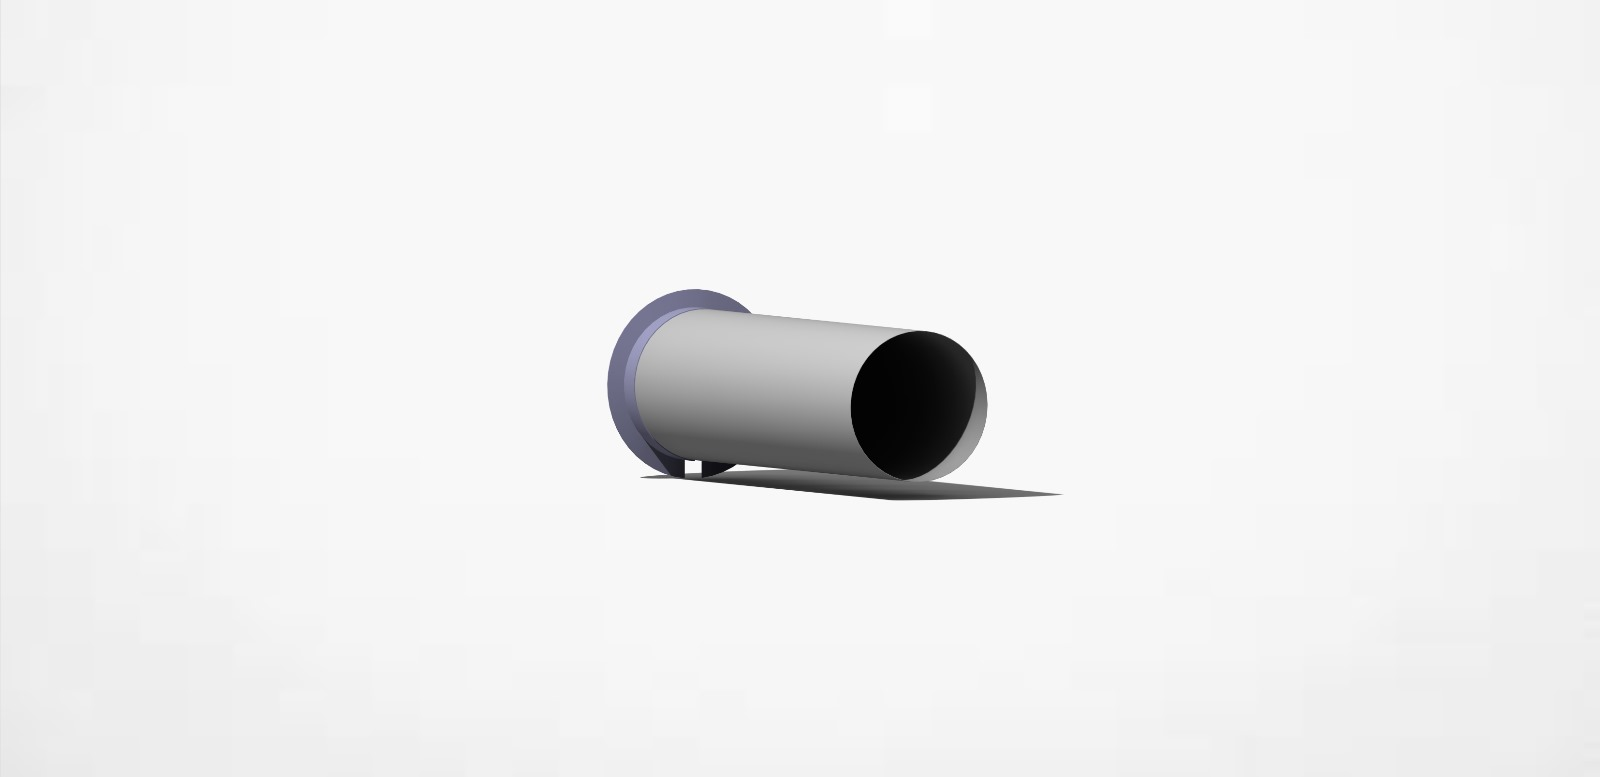
\includegraphics[width=2cm]{Figures/Montaje/2.jpg}};\\
 & \node[lablum=c]{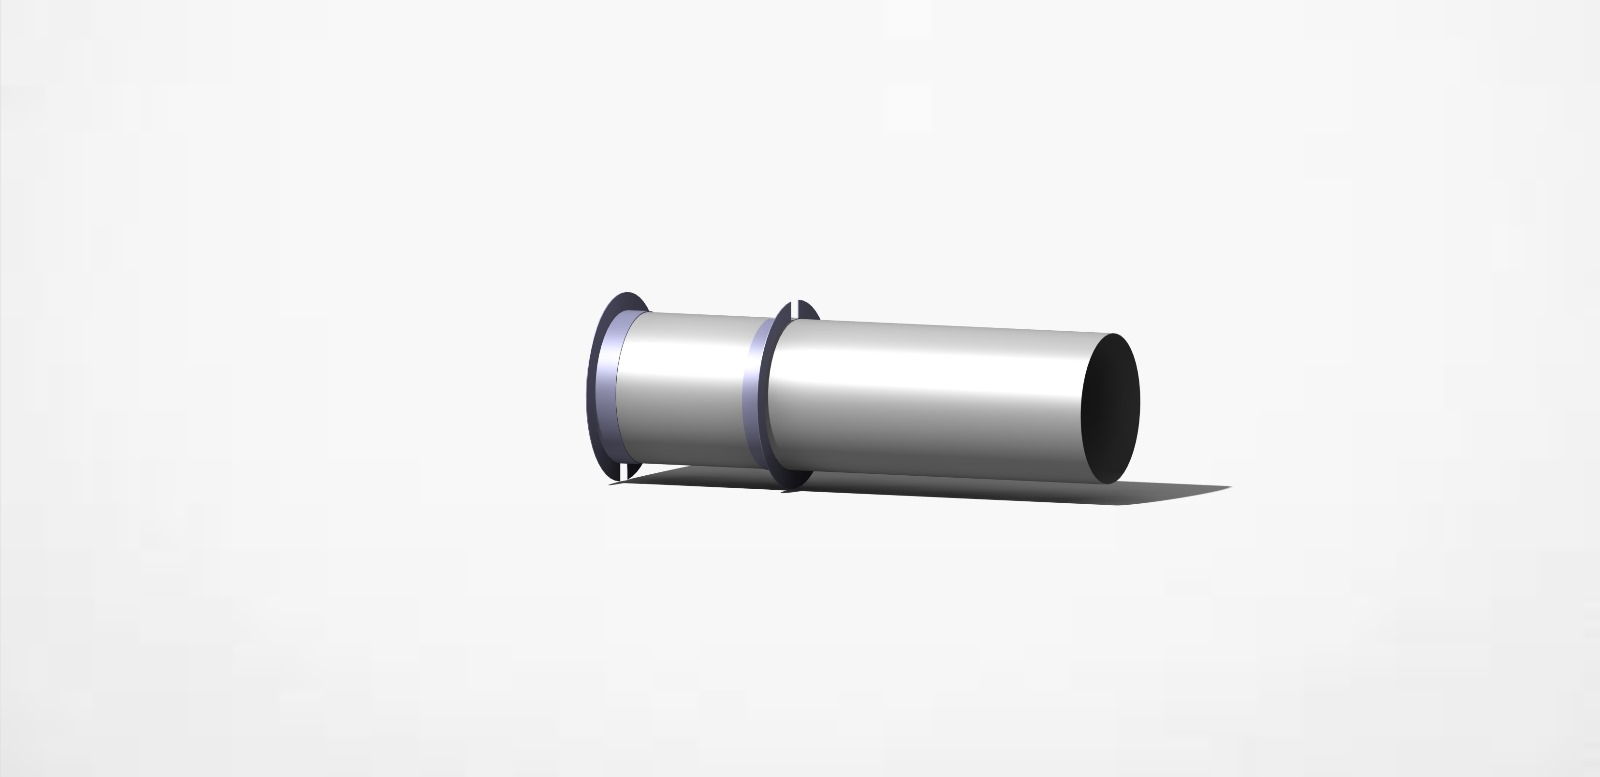
\includegraphics[width=2cm]{Figures/Montaje/3.jpg}};\\
 };
 \draw[marr] (img-a) -- (img-b);
 \draw[marr] ([xshift=1mm]img-b.south east) coordinate (aux) 
 -- (img-c.north-|aux);

\end{tikzpicture}
\caption{Primer Paso. \label{fig:primer}}
\end{figure}
%===============================================================================================================


\subsection{Segundo Paso: Introducción del Sombrerete Trasero}
Colocamos sobre el extremo del tubo de soporte el primer sombrerete, con las solapas hacia el interior del tubo. Se unirá mediante soldadura oxiacetilénica con material de aporte.

Ver figura \ref{fig:seg}.
%===============================================================================================================
%                                                   SEGUNDO PASO
%===============================================================================================================
\begin{figure}[!htb]
\centering
\begin{tikzpicture}[lablum/.style 2 args={label=below:#1 #2,name=img-#1},
marr/.style={line width=1mm,-latex}]
 \matrix[column sep=1cm,row sep=5mm] (mat)
 { \node[lablum={a}{}]{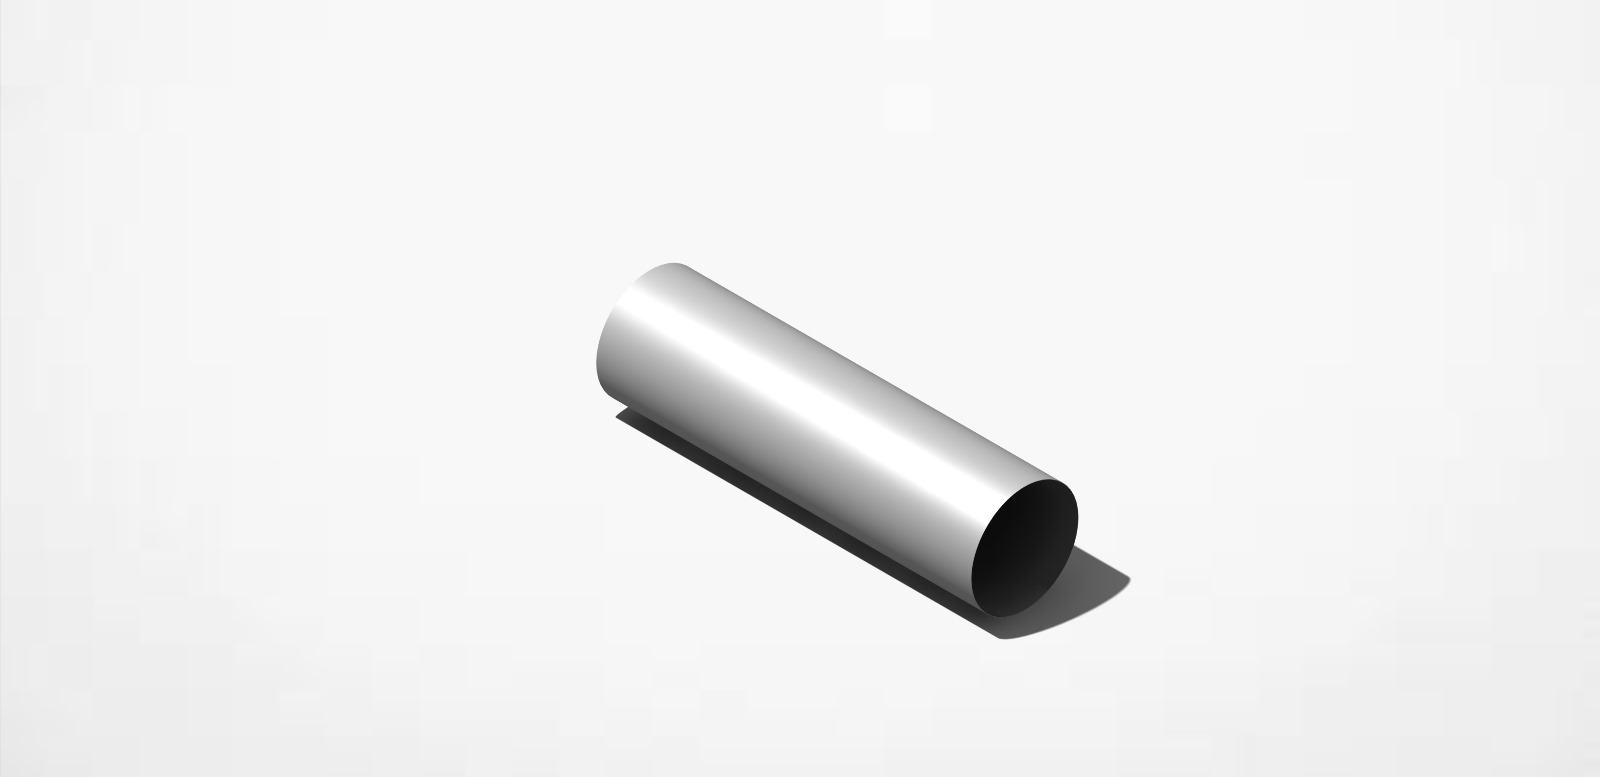
\includegraphics[width=2cm]{Figures/Montaje/1.jpg}};
 & \node[lablum={b}{}]{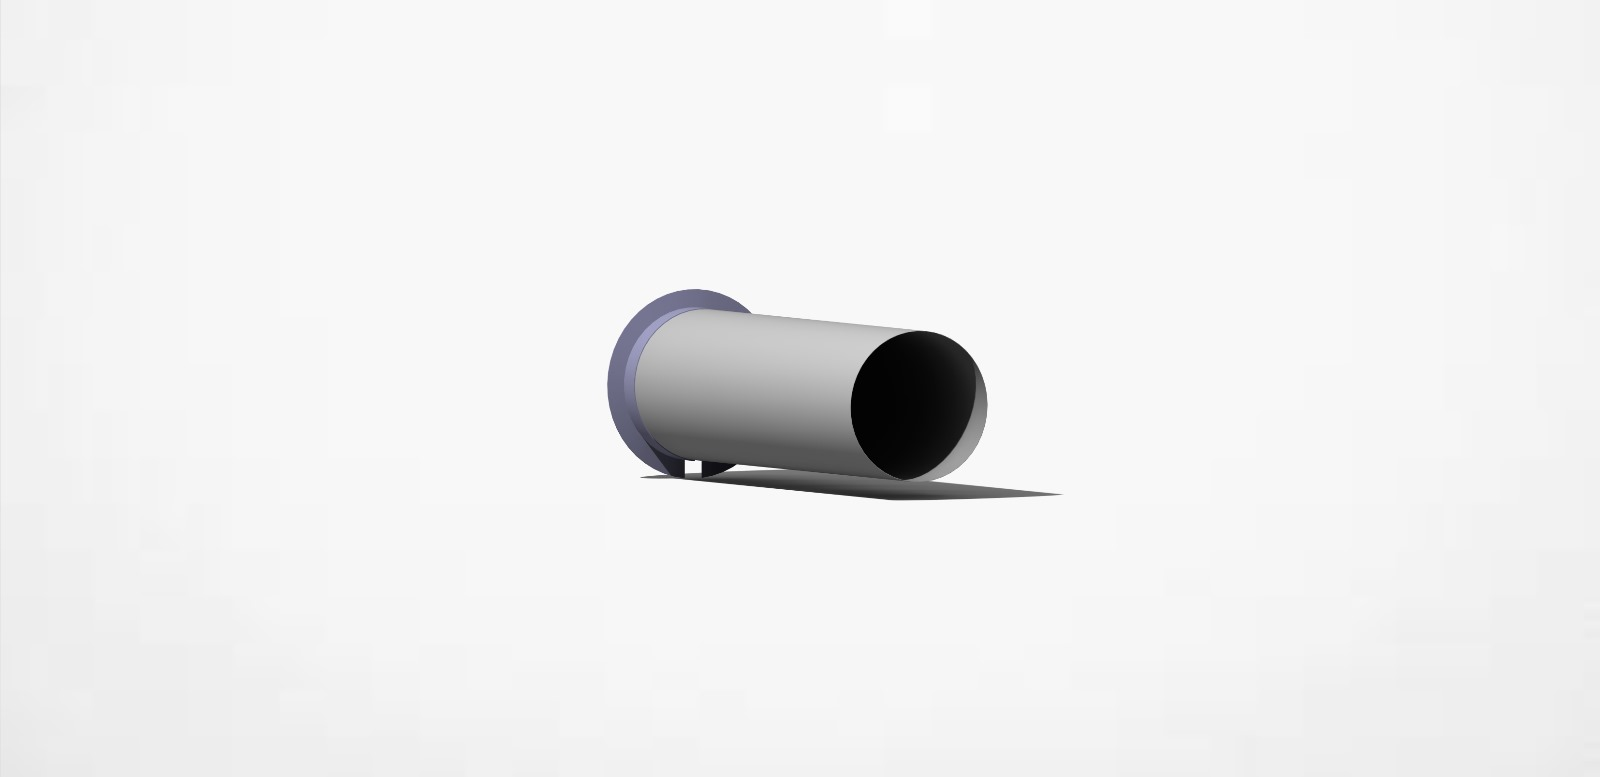
\includegraphics[width=5.5cm]{Figures/Montaje/2.jpg}};\\
 & \node[lablum=c]{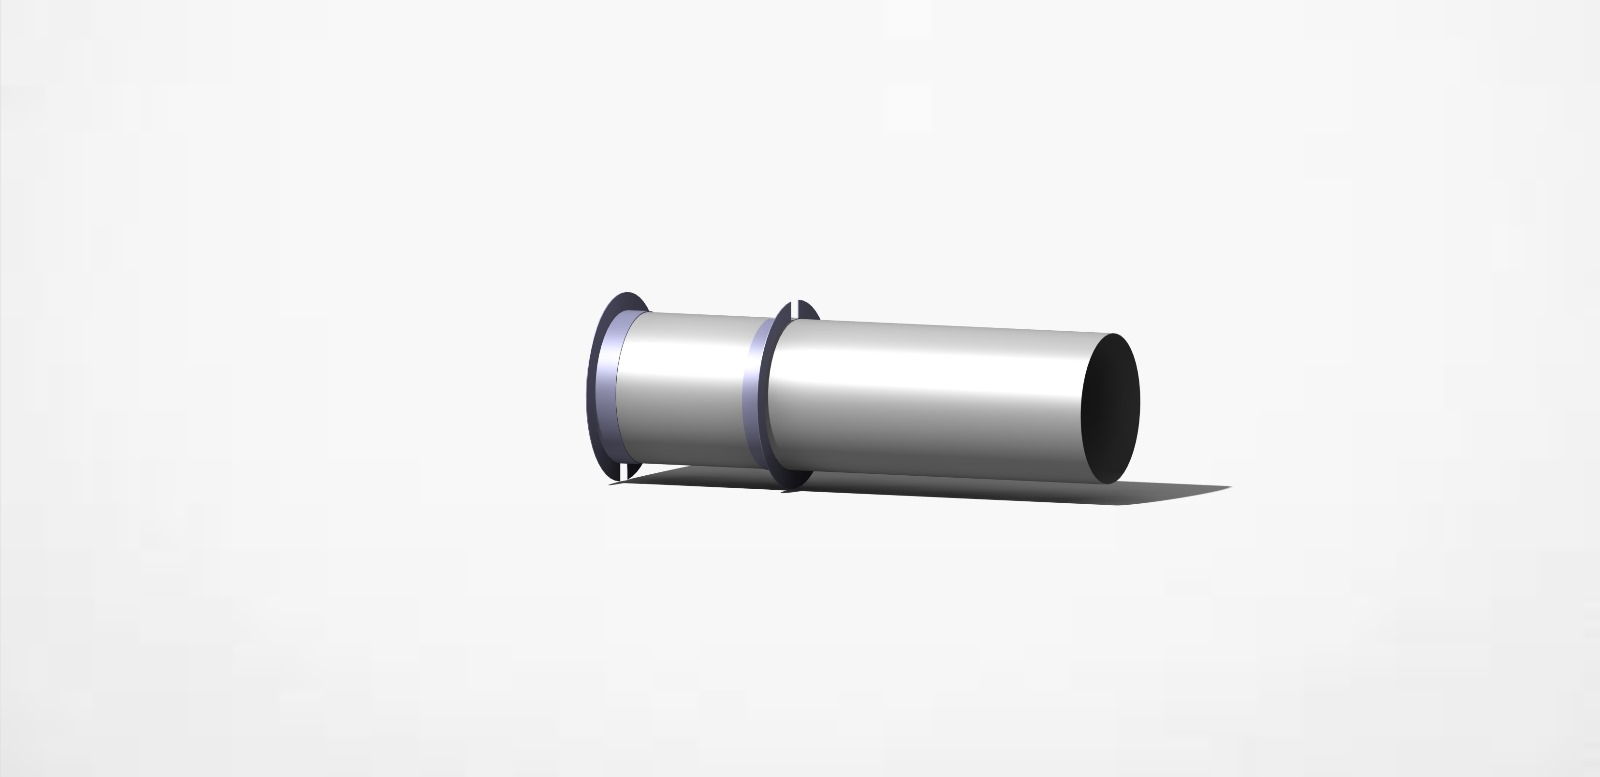
\includegraphics[width=2cm]{Figures/Montaje/3.jpg}};\\ 
 };
 \draw[marr] (img-a) -- (img-b);
 \draw[marr] ([xshift=1mm]img-b.south east) coordinate (aux) 
 -- (img-c.north-|aux);

\end{tikzpicture}
\caption{Segundo Paso. \label{fig:seg}}
\end{figure}
%===============================================================================================================


\subsection{Tercer Paso: Introducción del Sombrerete Intermedio}
Análogo al paso anterior, pero orientando las solapas hacia el primer sombrerete.

Ver figura \ref{fig:ter}

%===============================================================================================================
%                                                   TERCER PASO
%===============================================================================================================
\begin{figure}[!htb]
\centering
\begin{tikzpicture}[lablum/.style 2 args={label=below:#1 #2,name=img-#1},
marr/.style={line width=1mm,-latex}]
 \matrix[column sep=1cm,row sep=5mm] (mat)
 {  & \node[lablum={b}{}]{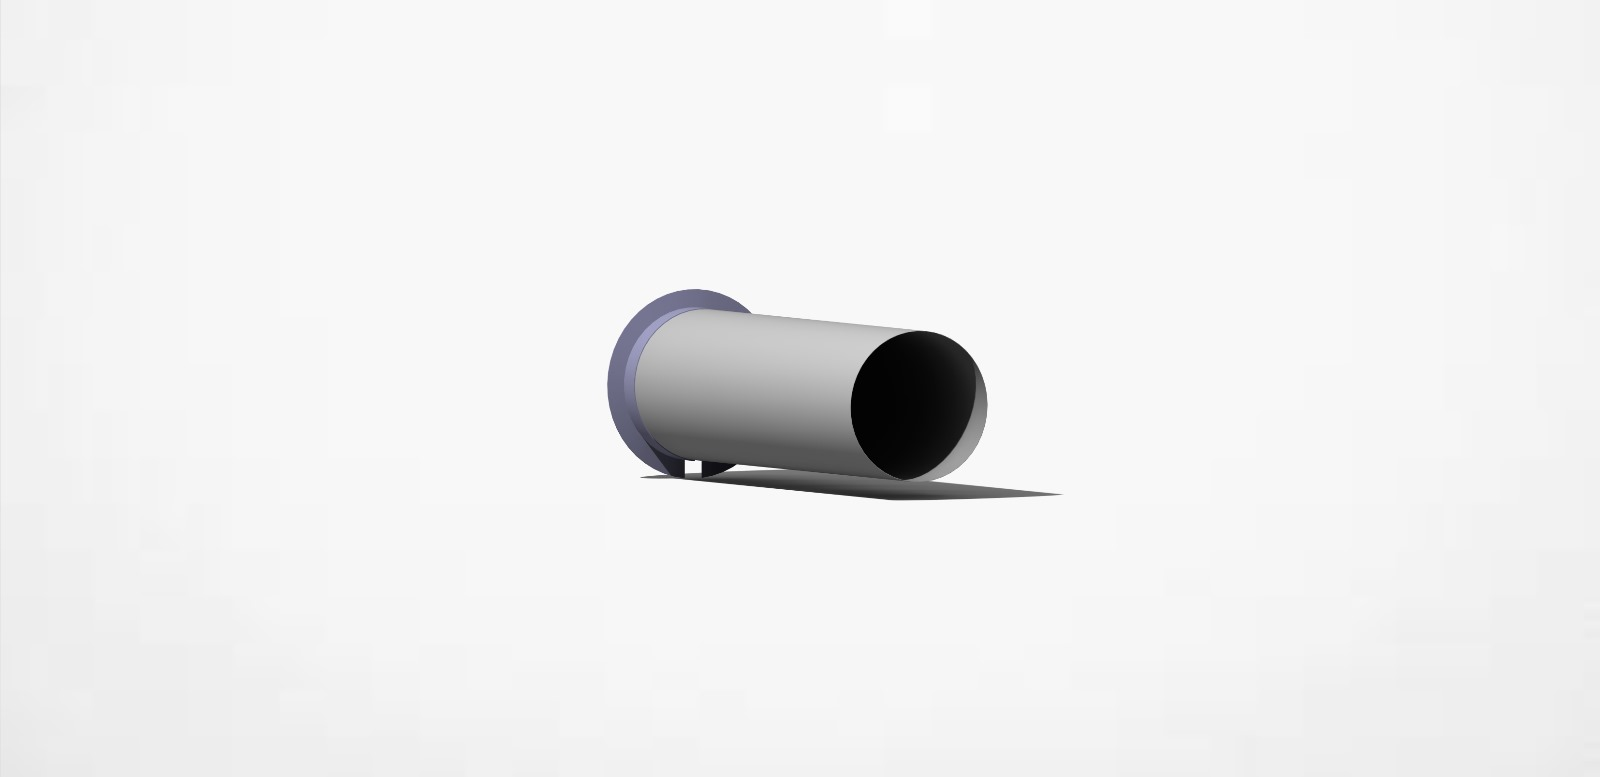
\includegraphics[width=2cm]{Figures/Montaje/2.jpg}};\\
 \node[lablum=d]{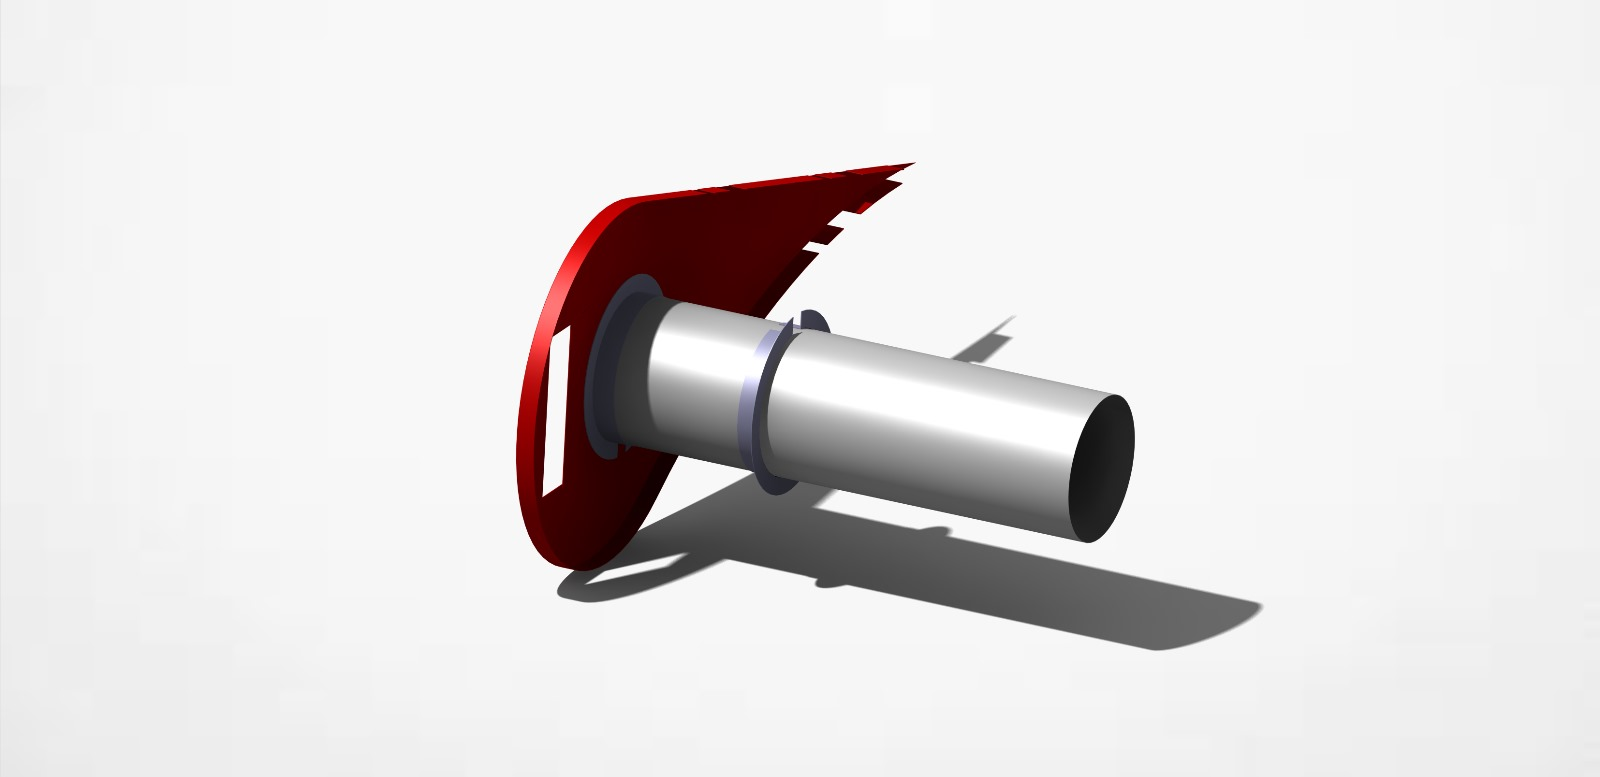
\includegraphics[width=2cm]{Figures/Montaje/4.jpg}};  & \node[lablum=c]{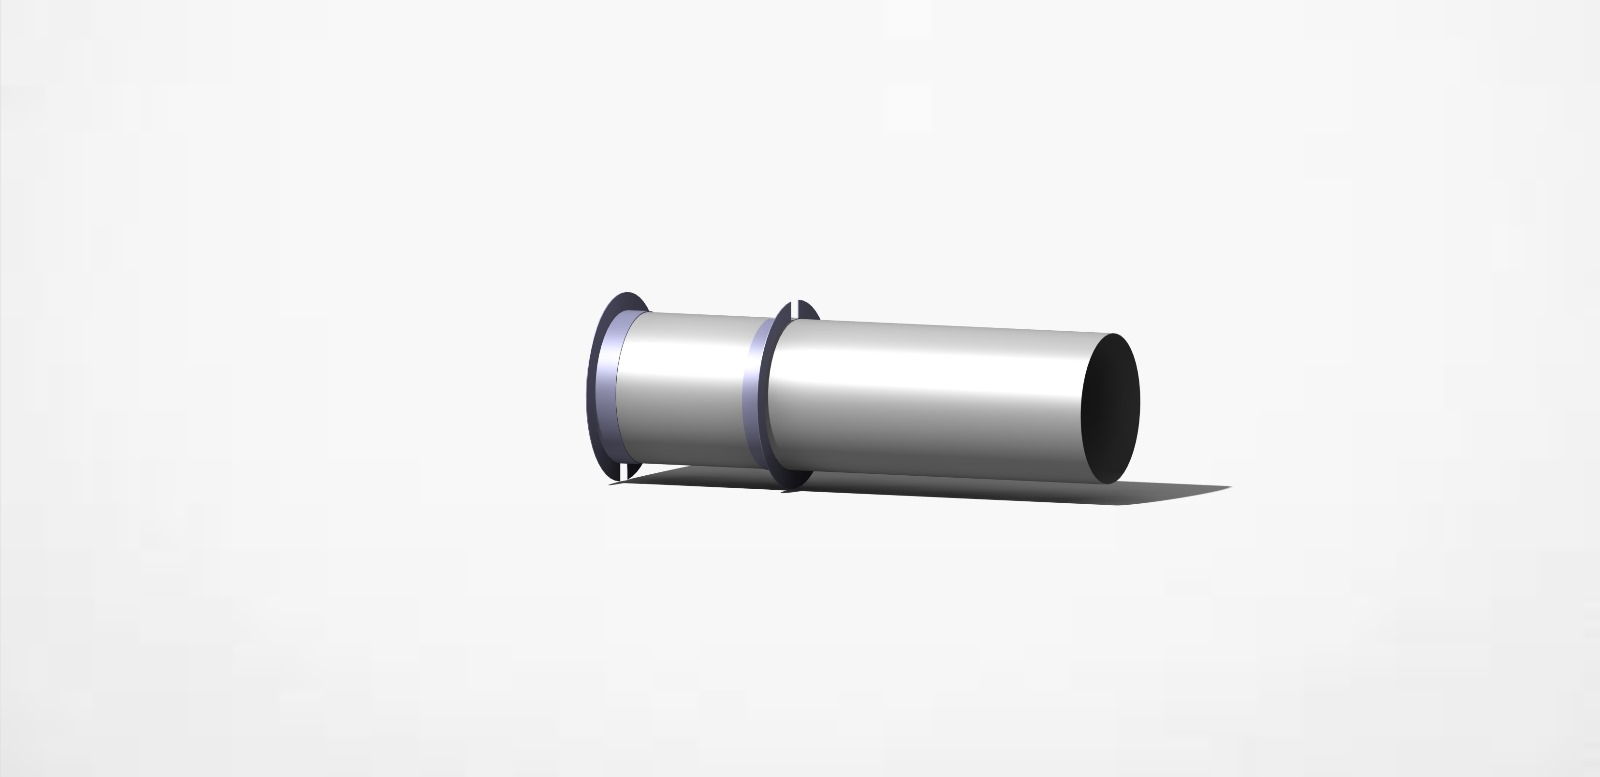
\includegraphics[width=5.5cm]{Figures/Montaje/3.jpg}};\\
 };
 \draw[marr] ([xshift=1mm]img-b.south east) coordinate (aux) 
 -- (img-c.north-|aux);
 \draw[marr] (img-c) -- (img-d);
\end{tikzpicture}
\caption{Tercer Paso. \label{fig:ter}}
\end{figure}
%===============================================================================================================


\subsection{Cuarto Paso: Introducción de la Costilla Trasera}
Colocamos la costilla trasera (la única sin perforar) sobre el primer sombrerete (la que está en el extremo del tubo), y trazamos, sobre la parte interior de ella, la posición del sombrerete, para realizar, posteriormente, la unión de sendas piezas mediante un revestimiento con caña maciza y cabeza universal.

La costilla quedará orientada hacia el interior de la estructura, al estar colocada en el exterior del sombrerete.

Ver figura \ref{fig:cua}.

%===============================================================================================================
%                                                   CUARTO PASO
%===============================================================================================================
\begin{figure}[!htb]
\centering
\begin{tikzpicture}[lablum/.style 2 args={label=below:#1 #2,name=img-#1},
marr/.style={line width=1mm,-latex}]
 \matrix[column sep=1cm,row sep=5mm] (mat)
 { \node[lablum=d]{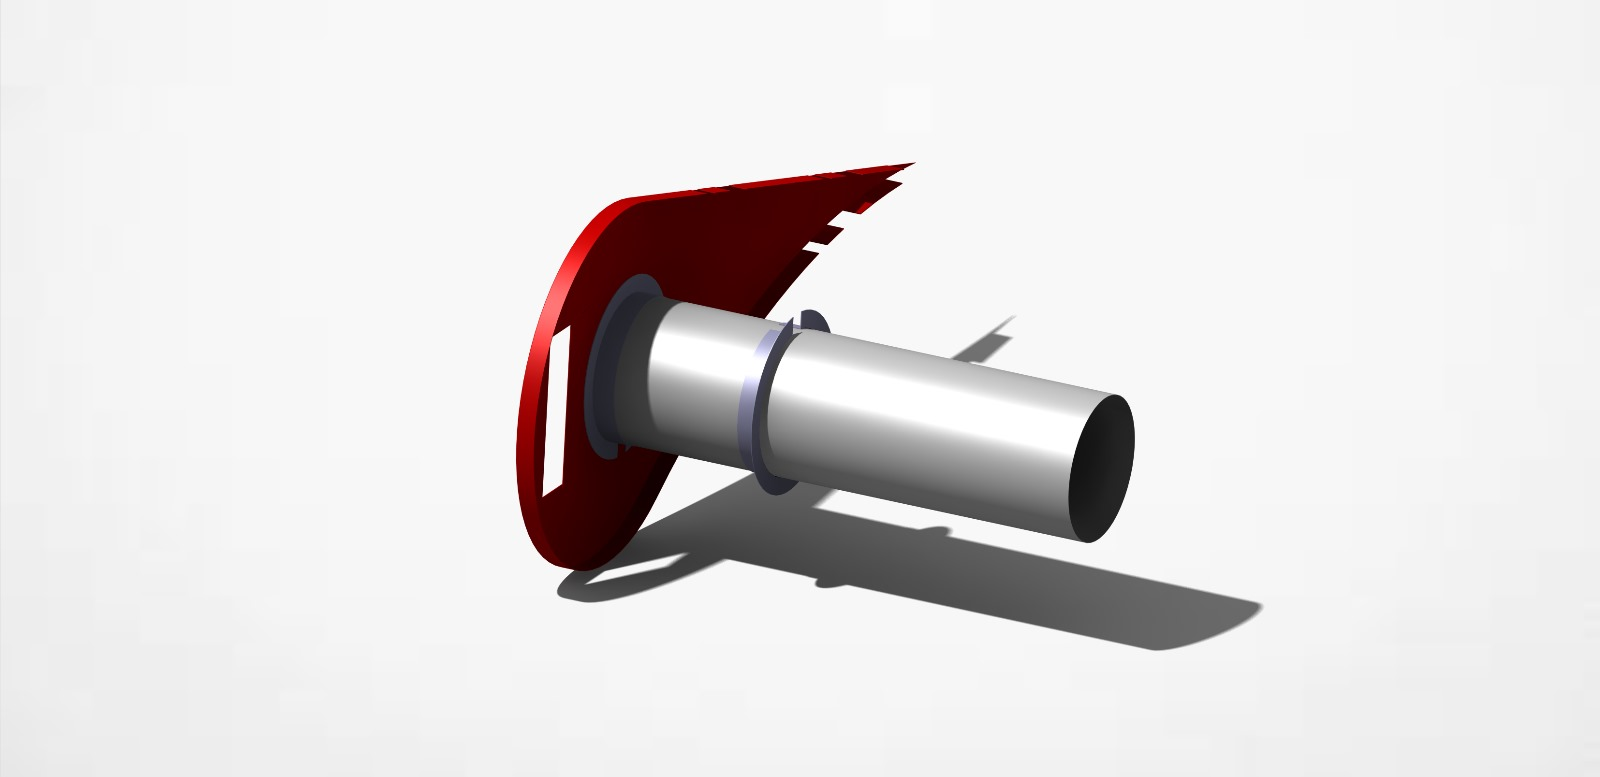
\includegraphics[width=5.5cm]{Figures/Montaje/4.jpg}};  & \node[lablum=c]{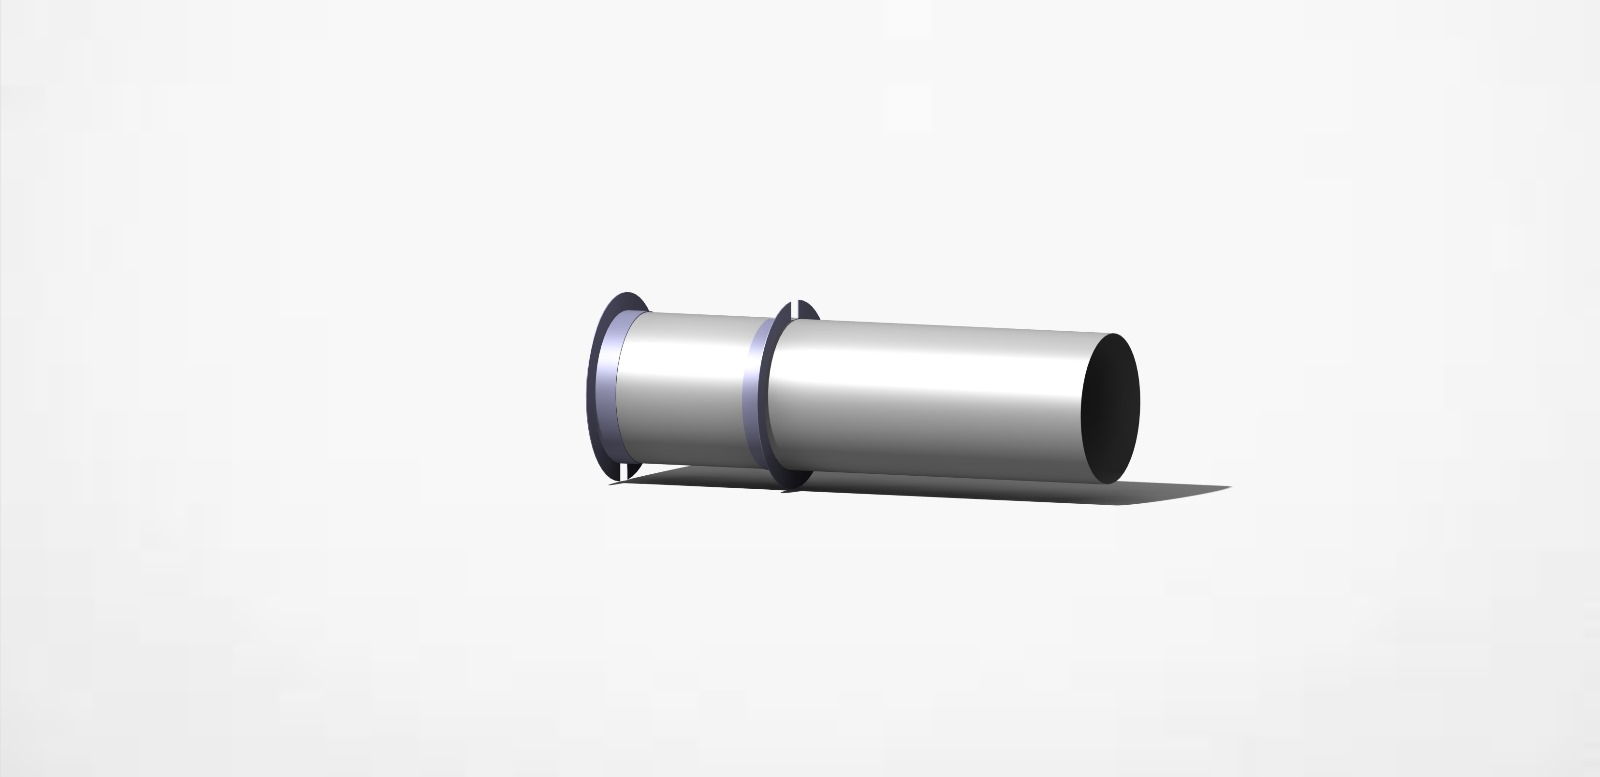
\includegraphics[width=2cm]{Figures/Montaje/3.jpg}};\\
 \node[lablum=e]{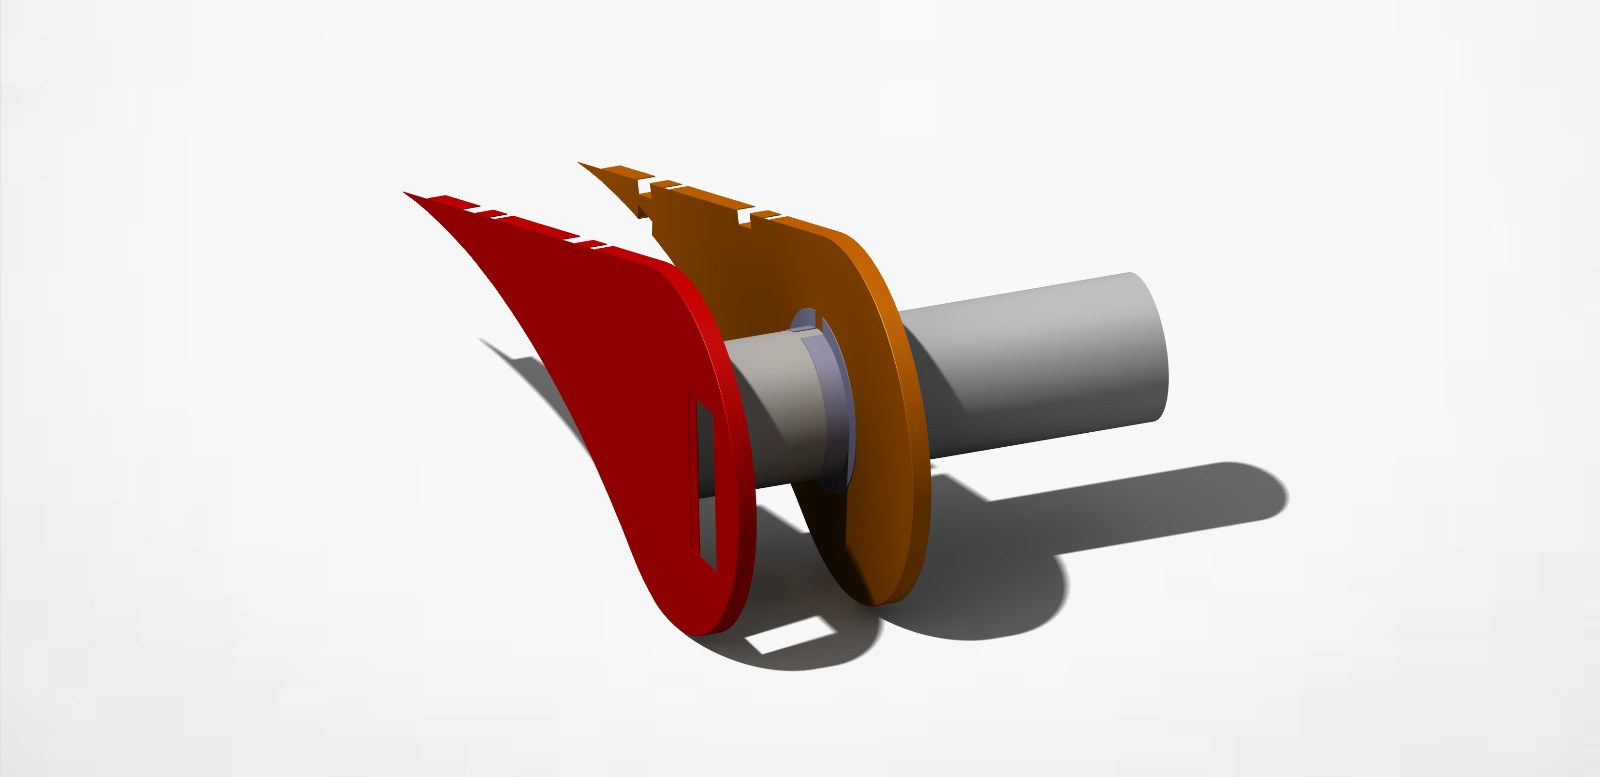
\includegraphics[width=2cm]{Figures/Montaje/5.jpg}};
 & \\
 };
 \draw[marr] (img-c) -- (img-d);
  \draw[marr] ([xshift=-1mm]img-d.south west) coordinate (aux) 
 -- (img-e.north-|aux);
\end{tikzpicture}
\caption{Cuarto Paso. \label{fig:cua}}
\end{figure}

\begin{nota}{Comentario sobre los Próximos Pasos}{}
    Antes de proceder con el Quinto Paso, apoyaremos sobre la mesa de trabajo la parte recta del perfil de trabajo (el correspondiente con el extradós). Haremos esto con el fin de garantizar que todas las costillas queden alineadas correctamente.
\end{nota}
%===============================================================================================================


\subsection{Quinto Paso: Introducción de la Costilla Intermedia}
Análogo al paso anterior.

Ver figura \ref{fig:qui}.
%===============================================================================================================
%                                                   QUINTO PASO
%===============================================================================================================
\begin{figure}[!htb]
\centering
\begin{tikzpicture}[lablum/.style 2 args={label=below:#1 #2,name=img-#1},
marr/.style={line width=1mm,-latex}]
 \matrix[column sep=1cm,row sep=5mm] (mat)
 { \node[lablum=d]{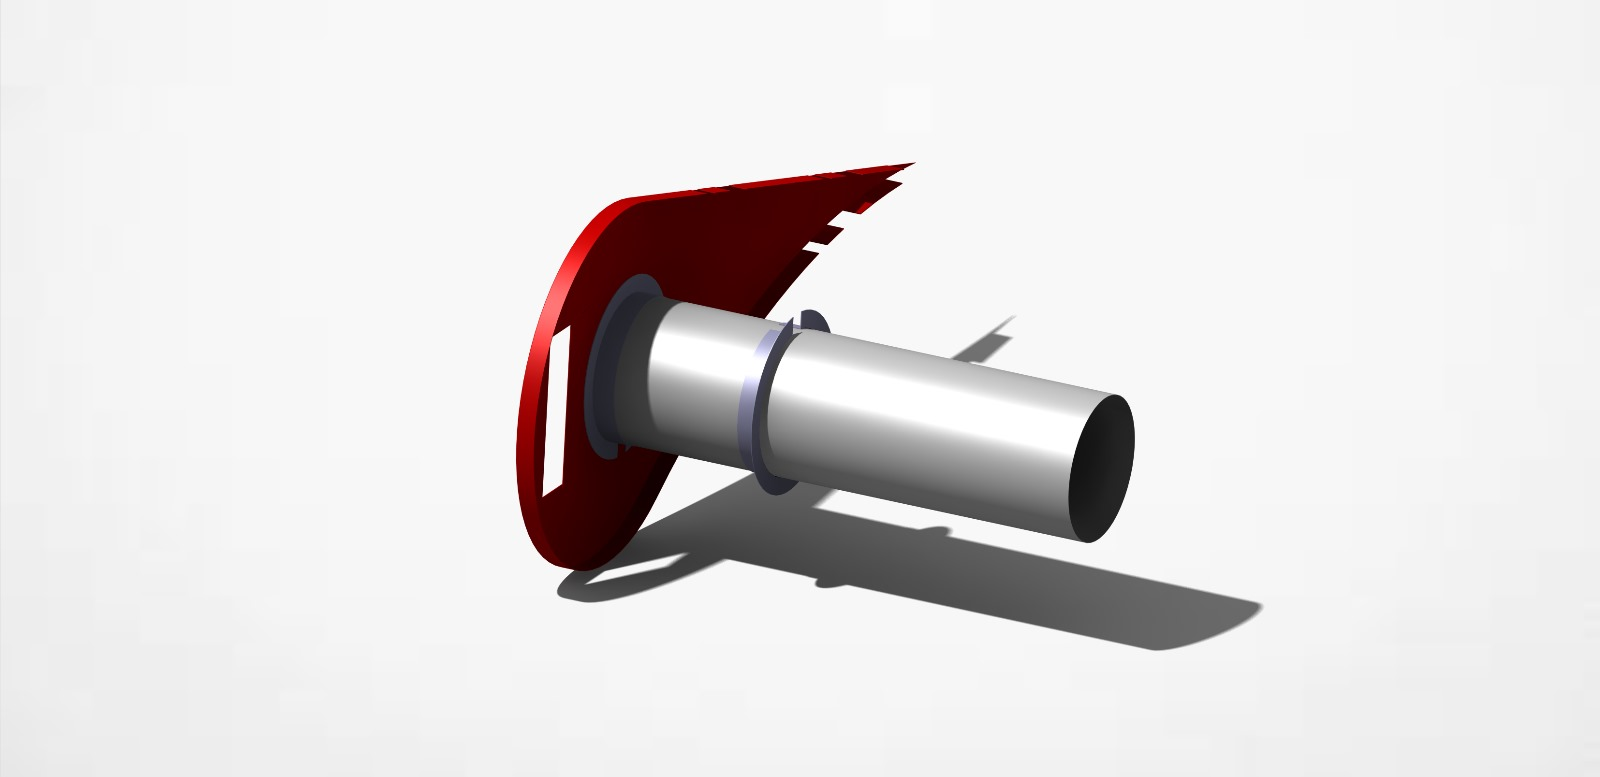
\includegraphics[width=2cm]{Figures/Montaje/4.jpg}}; \\
 \node[lablum=e]{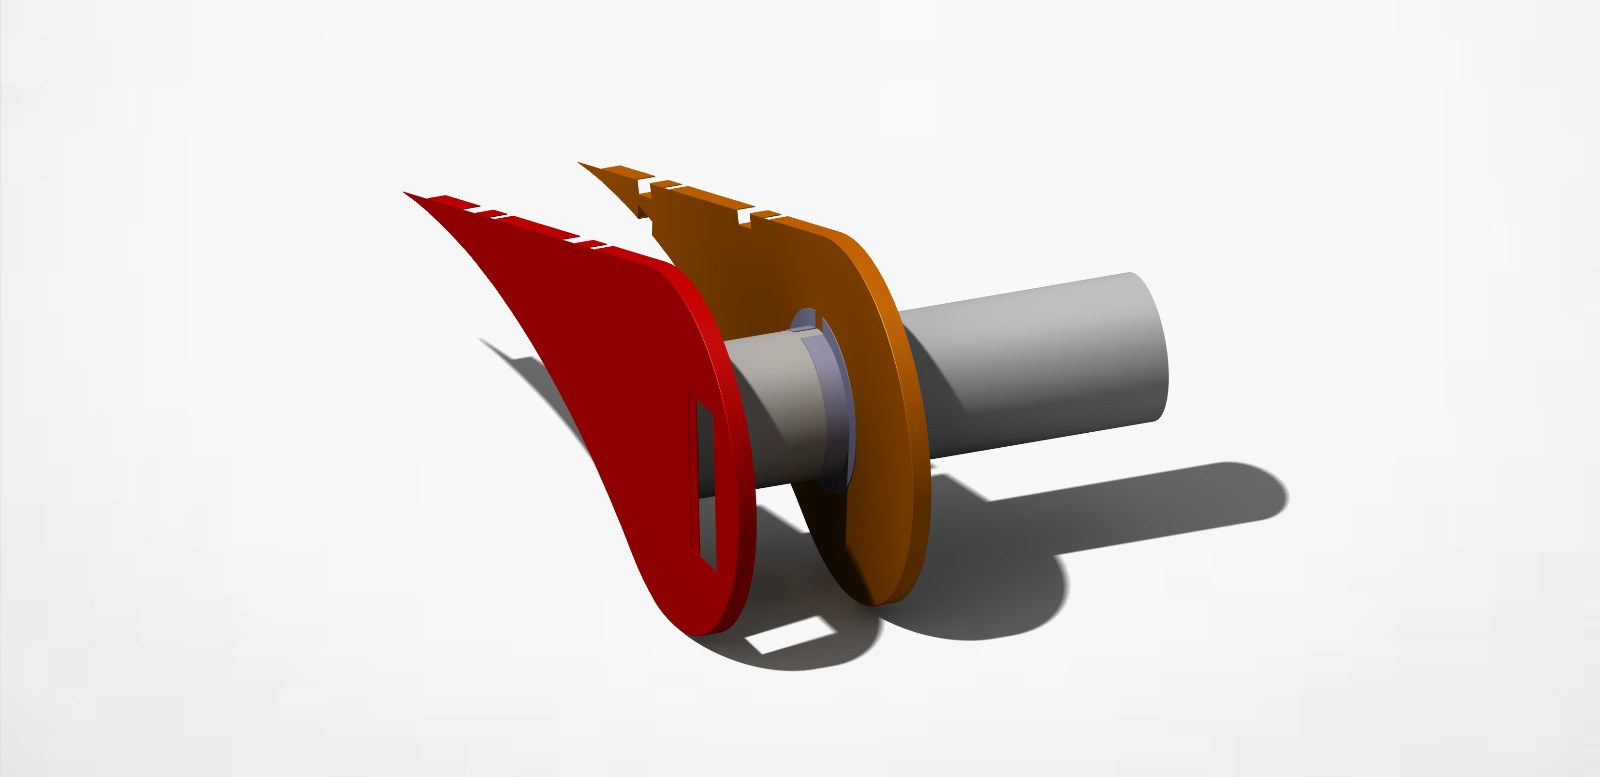
\includegraphics[width=5.5cm]{Figures/Montaje/5.jpg}}; & \node[lablum=f]{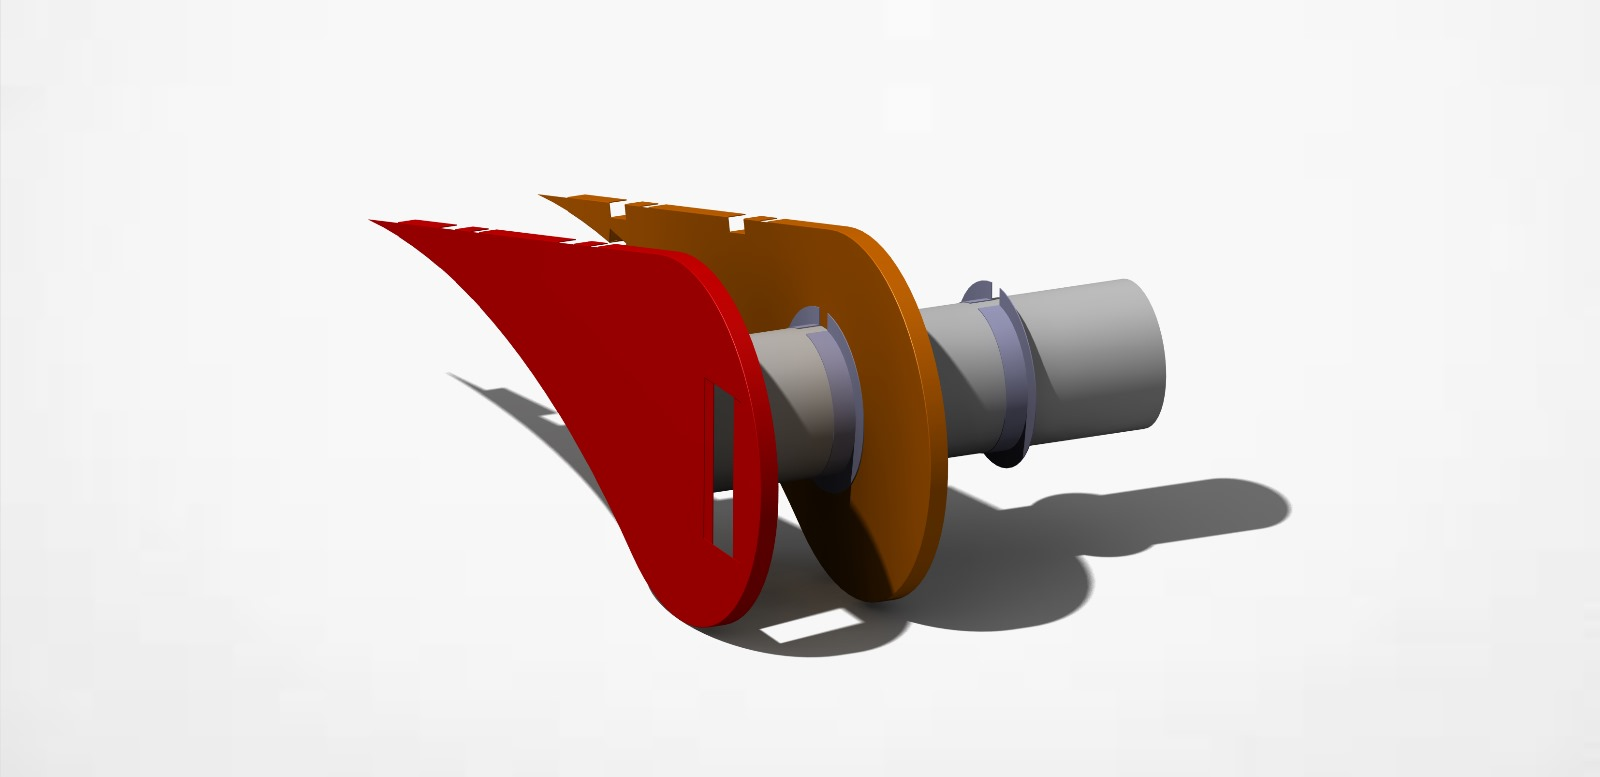
\includegraphics[width=2cm]{Figures/Montaje/6.jpg}}; \\
 };
  \draw[marr] ([xshift=-1mm]img-d.south west) coordinate (aux) 
 -- (img-e.north-|aux);
 \draw[marr] (img-e) -- (img-f);
\end{tikzpicture}
\caption{Quinto Paso. \label{fig:qui}}
\end{figure}
%===============================================================================================================

\pagebreak

\subsection{Sexto Paso: Introducción del Sombrerete Delantero}
Análogo a los pasos Segundo y Tercero.

Ver figura \ref{fig:sex}.

%===============================================================================================================
%                                                   SEXTO PASO
%===============================================================================================================
\begin{figure}[!htb]
\centering
\begin{tikzpicture}[lablum/.style 2 args={label=below:#1 #2,name=img-#1},
marr/.style={line width=1mm,-latex}]
 \matrix[column sep=1cm,row sep=5mm] (mat)
 {  \node[lablum=e]{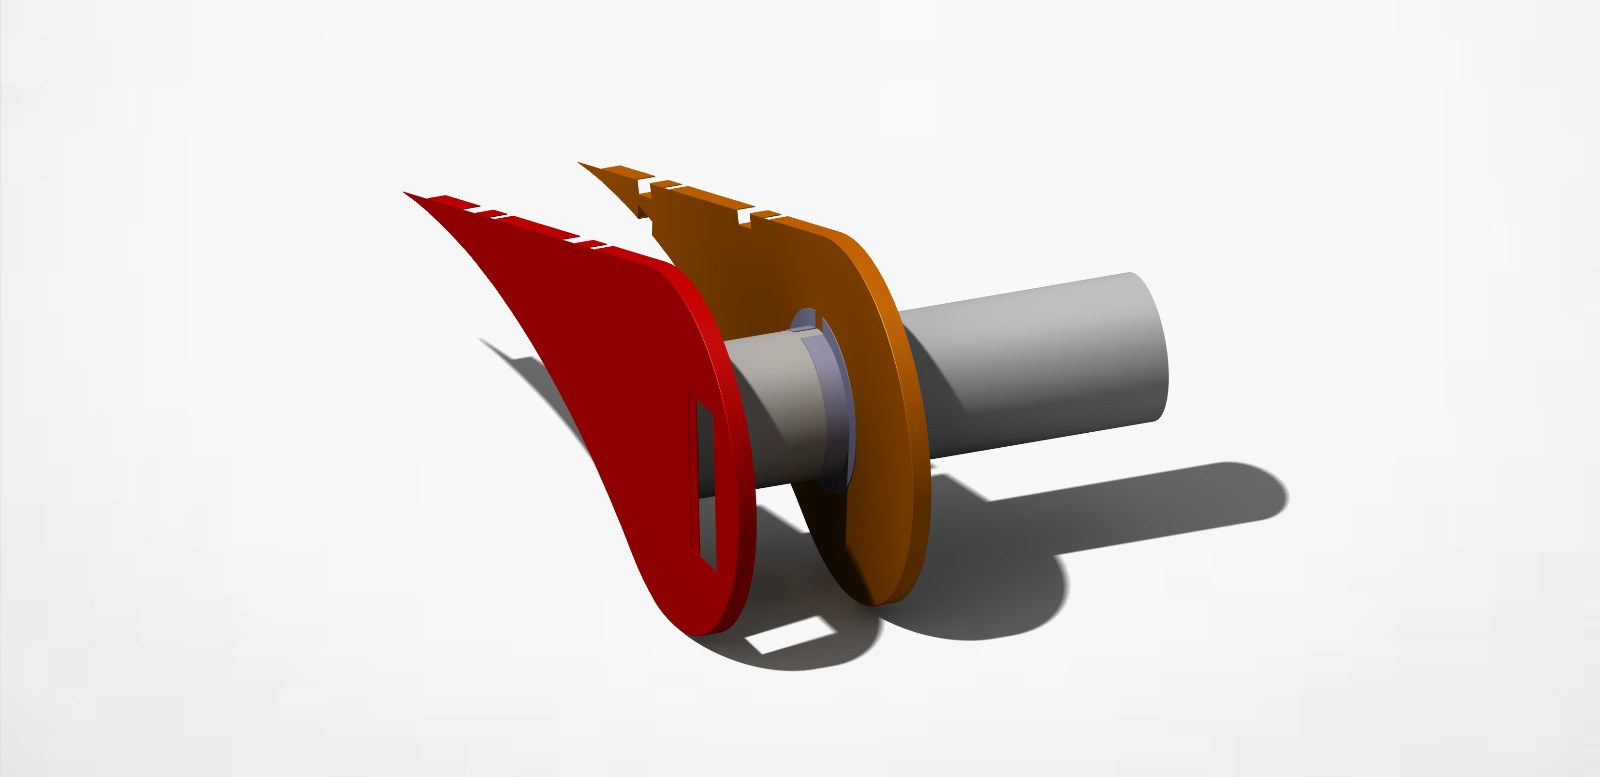
\includegraphics[width=2cm]{Figures/Montaje/5.jpg}}; & \node[lablum=f]{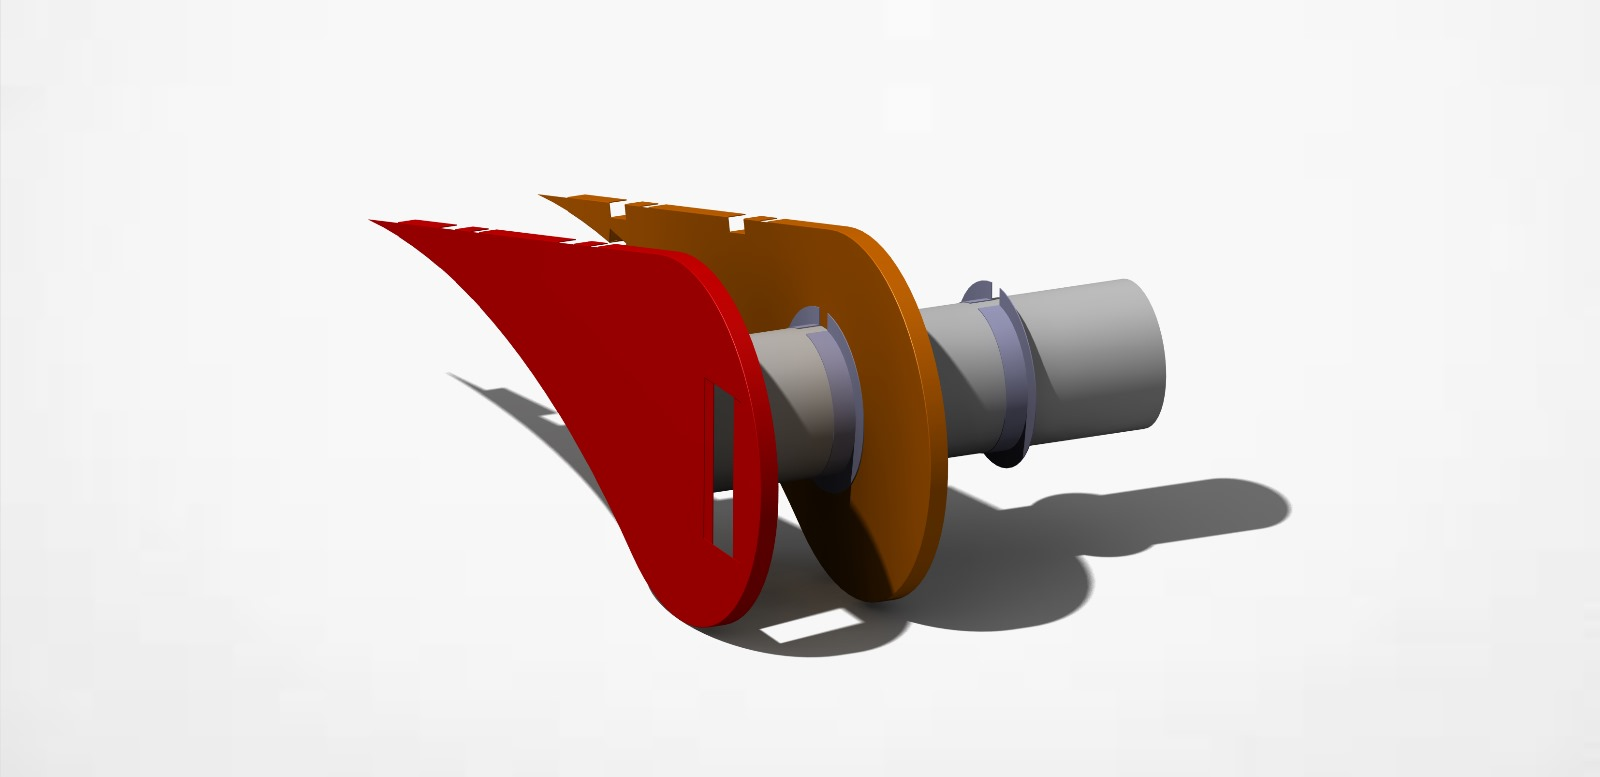
\includegraphics[width=5.5cm]{Figures/Montaje/6.jpg}}; \\
  & \node[lablum=g]{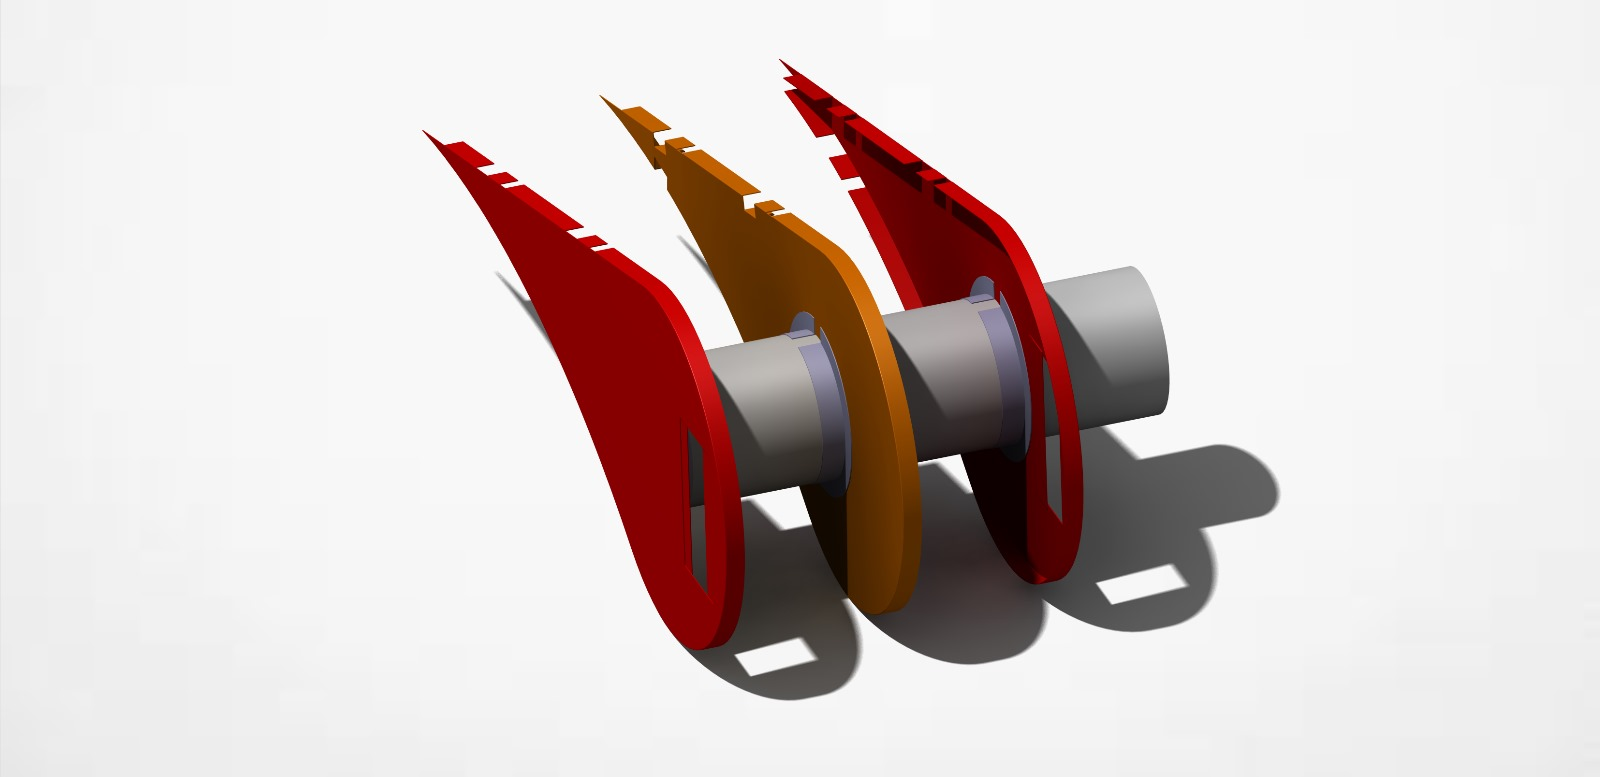
\includegraphics[width=2cm]{Figures/Montaje/7.jpg}};\\ 
 };
 \draw[marr] (img-e) -- (img-f);
  \draw[marr] ([xshift=-1mm]img-f.south east) coordinate (aux) 
 -- (img-g.north-|aux);
\end{tikzpicture}
\caption{Sexto Paso. \label{fig:sex}}
\end{figure}
%===============================================================================================================

\subsection{Séptimo Paso: Unión de la Costilla Delantera}
Se efectúa la unión de la costilla delantera con su sombrerete correspondiente.

Recordemos que la costilla ha de quedar orientada hacia el interior, pero situada al exterior del sombrerete.

Ver figura \ref{fig:sept}.

%===============================================================================================================
%                                                 SÉPTIMO PASO
%===============================================================================================================
\begin{figure}[!htb]
\centering
\begin{tikzpicture}[lablum/.style 2 args={label=below:#1 #2,name=img-#1},
marr/.style={line width=1mm,-latex}]
 \matrix[column sep=1cm,row sep=5mm] (mat)
 {   & \node[lablum=f]{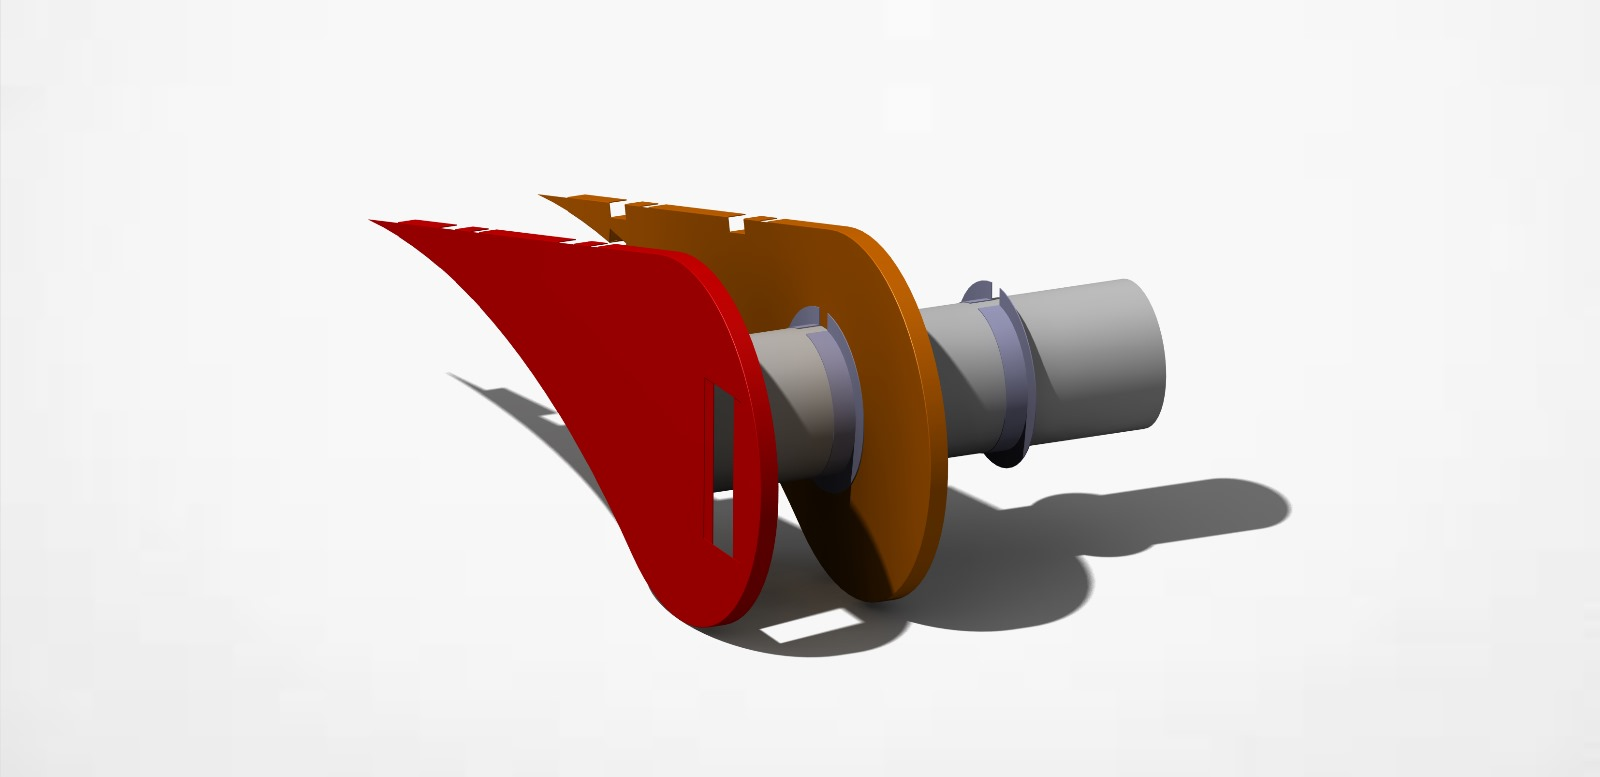
\includegraphics[width=2cm]{Figures/Montaje/6.jpg}}; \\
  \node[lablum=h]{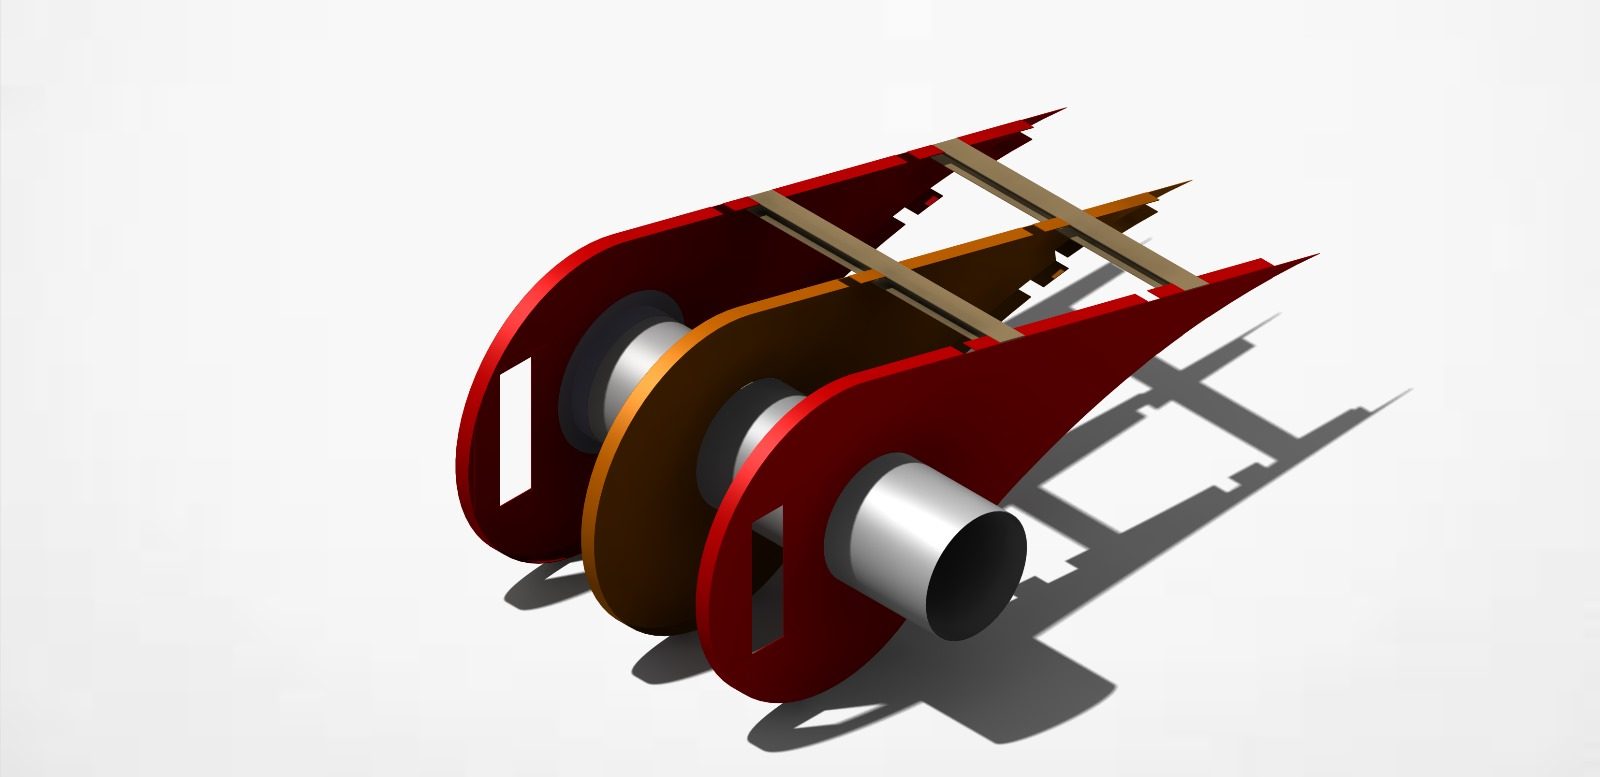
\includegraphics[width=2cm]{Figures/Montaje/8.jpg}}; & \node[lablum=g]{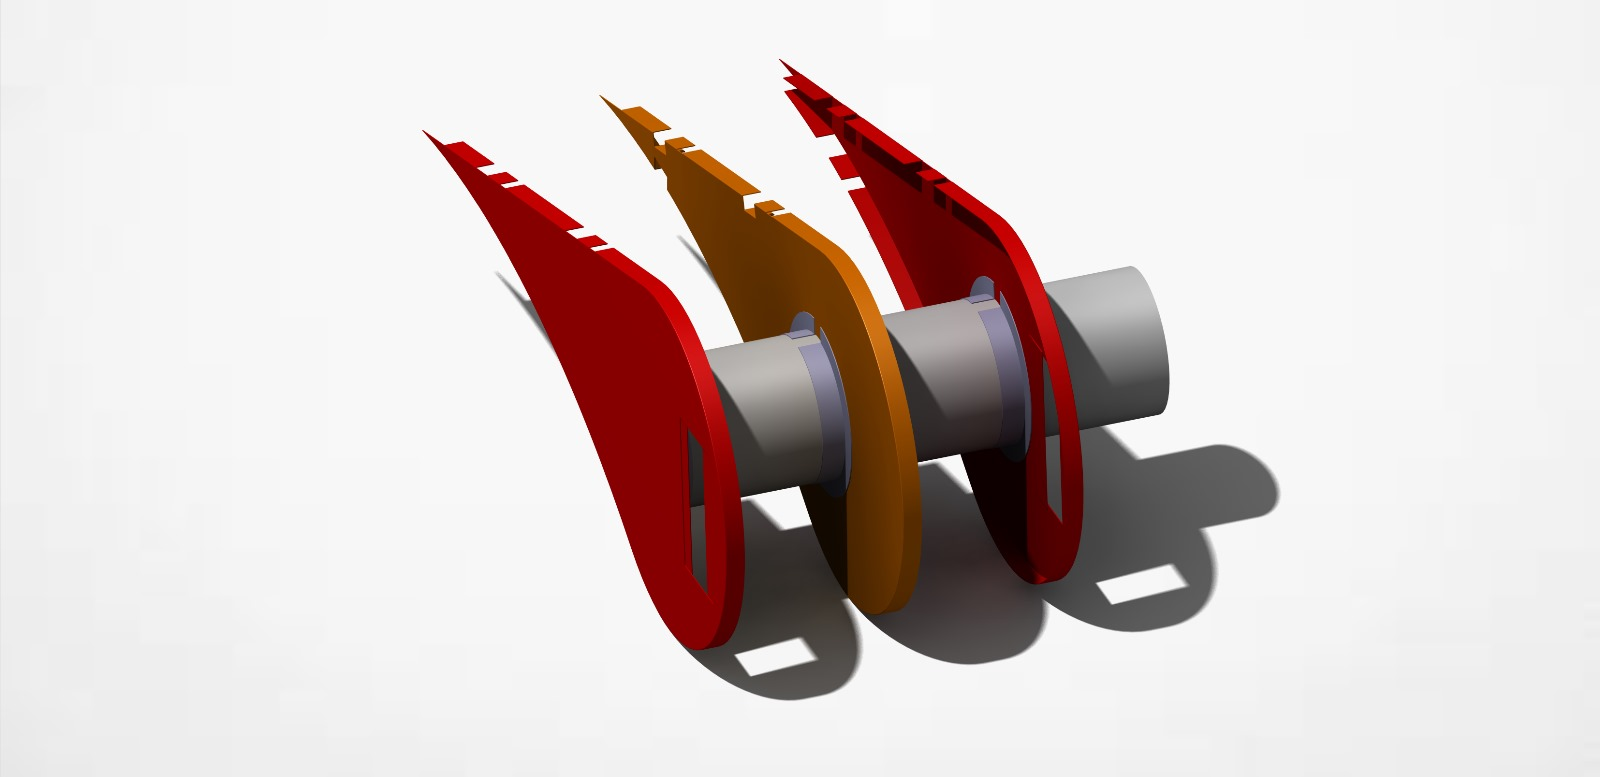
\includegraphics[width=5.5cm]{Figures/Montaje/7.jpg}}; \\
 };
\draw[marr] ([xshift=-1mm]img-f.south east) coordinate (aux) 
 -- (img-g.north-|aux);
 \draw[marr] (img-g) -- (img-h);
\end{tikzpicture}
\caption{Séptimo Paso. \label{fig:sept}}
\end{figure}
%===============================================================================================================


\subsection{Octavo y Noveno Pasos: Larguerillos}
Introducimos cuatro larguerillos, dos superiores (Paso Octavo) y dos inferiores (Paso Noveno), de 398 [mm] en la estructura. Se colocarán sobre las ranuras de las costillas, y se unirán a ellas mediante soldadura por puntos.

Los larguerillos son necesarios ya que ayudan a mantener la integridad de la estructura.

Ver figuras \ref{fig:oct} y \ref{fig:nov}.

%===============================================================================================================
%                                                   OCTAVO PASO
%===============================================================================================================


\begin{figure}[!htb]
\centering
\begin{tikzpicture}[lablum/.style 2 args={label=below:#1 #2,name=img-#1},
marr/.style={line width=1mm,-latex}]
 \matrix[column sep=1cm,row sep=5mm] (mat)
 {   
  \node[lablum=h]{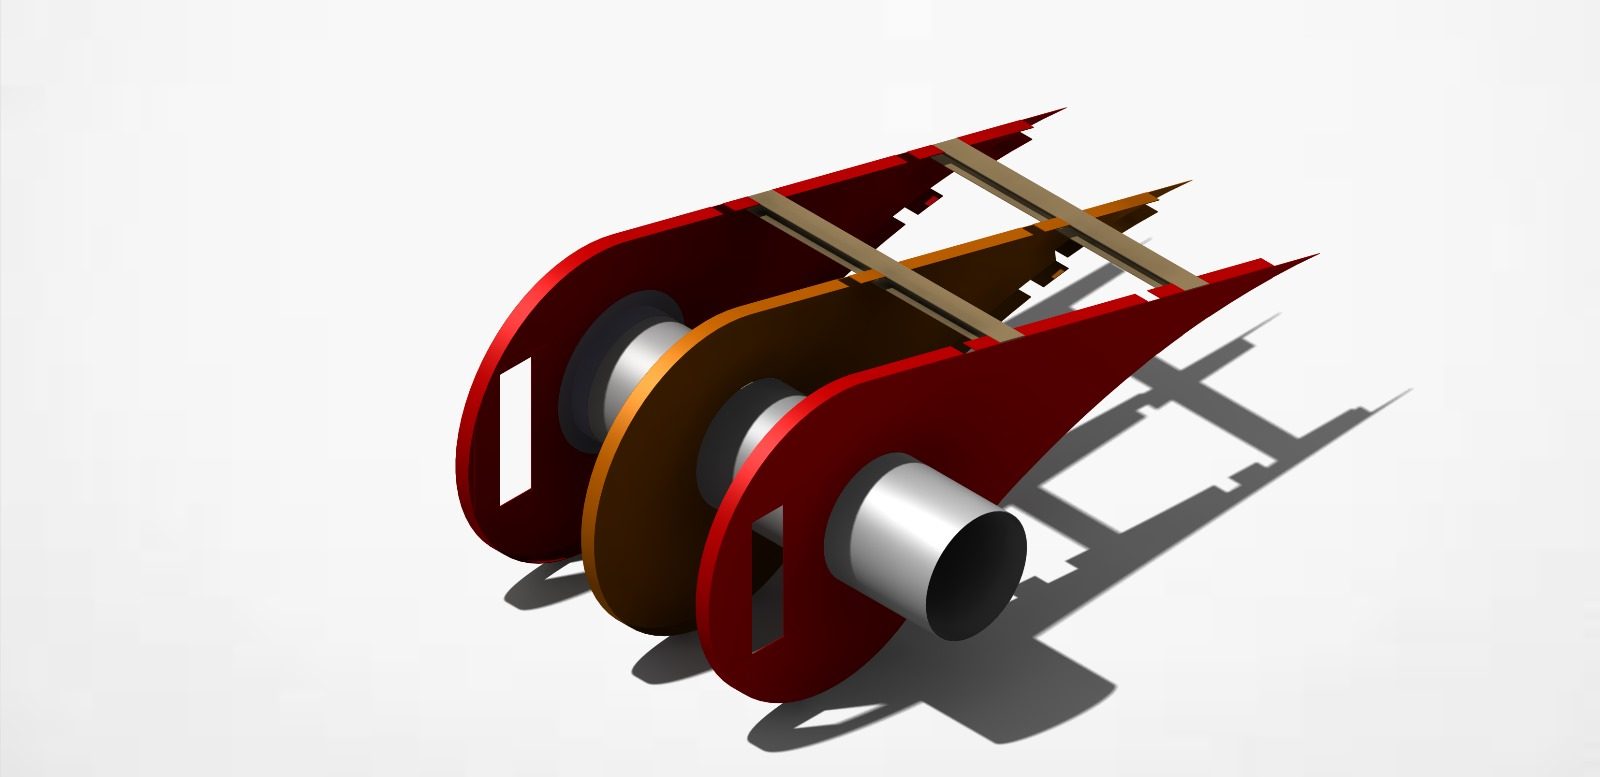
\includegraphics[width=5.5cm]{Figures/Montaje/8.jpg}}; & \node[lablum=g]{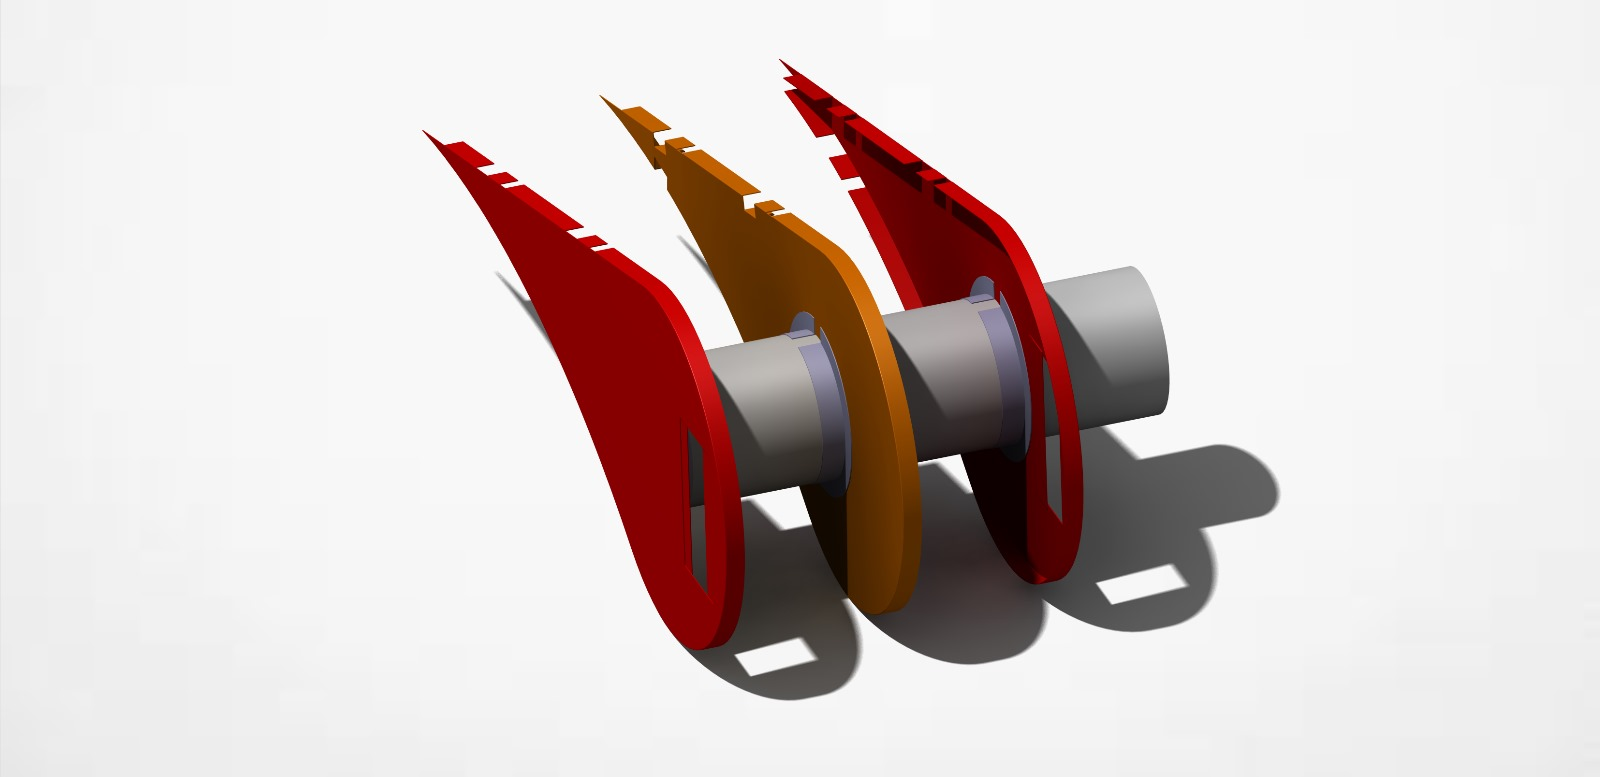
\includegraphics[width=2cm]{Figures/Montaje/7.jpg}};\\  \node[lablum=i]{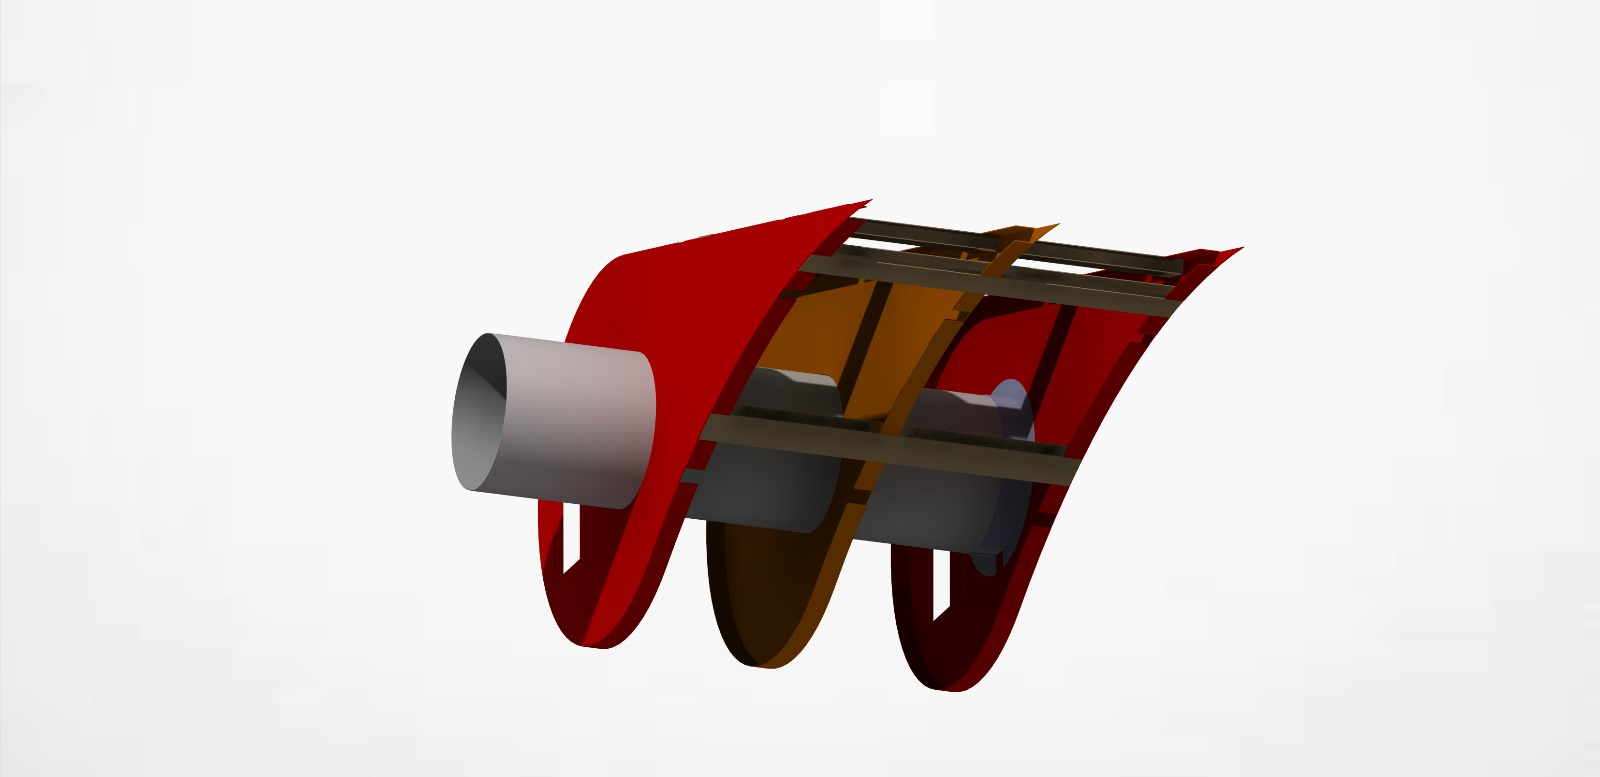
\includegraphics[width=2cm]{Figures/Montaje/9.jpg}}; \\
 };
 \draw[marr] (img-g) -- (img-h);
  \draw[marr] ([xshift=1mm]img-h.south west) coordinate (aux) 
 -- (img-i.north-|aux);
\end{tikzpicture}
\caption{Octavo Paso. \label{fig:oct}}
\end{figure}
%===============================================================================================================

%===============================================================================================================
%                                                   NOVENO PASO
%===============================================================================================================
\begin{figure}[!htb]
\centering
\begin{tikzpicture}[lablum/.style 2 args={label=below:#1 #2,name=img-#1},
marr/.style={line width=1mm,-latex}]
 \matrix[column sep=1cm,row sep=5mm] (mat)
 {   
  \node[lablum=h]{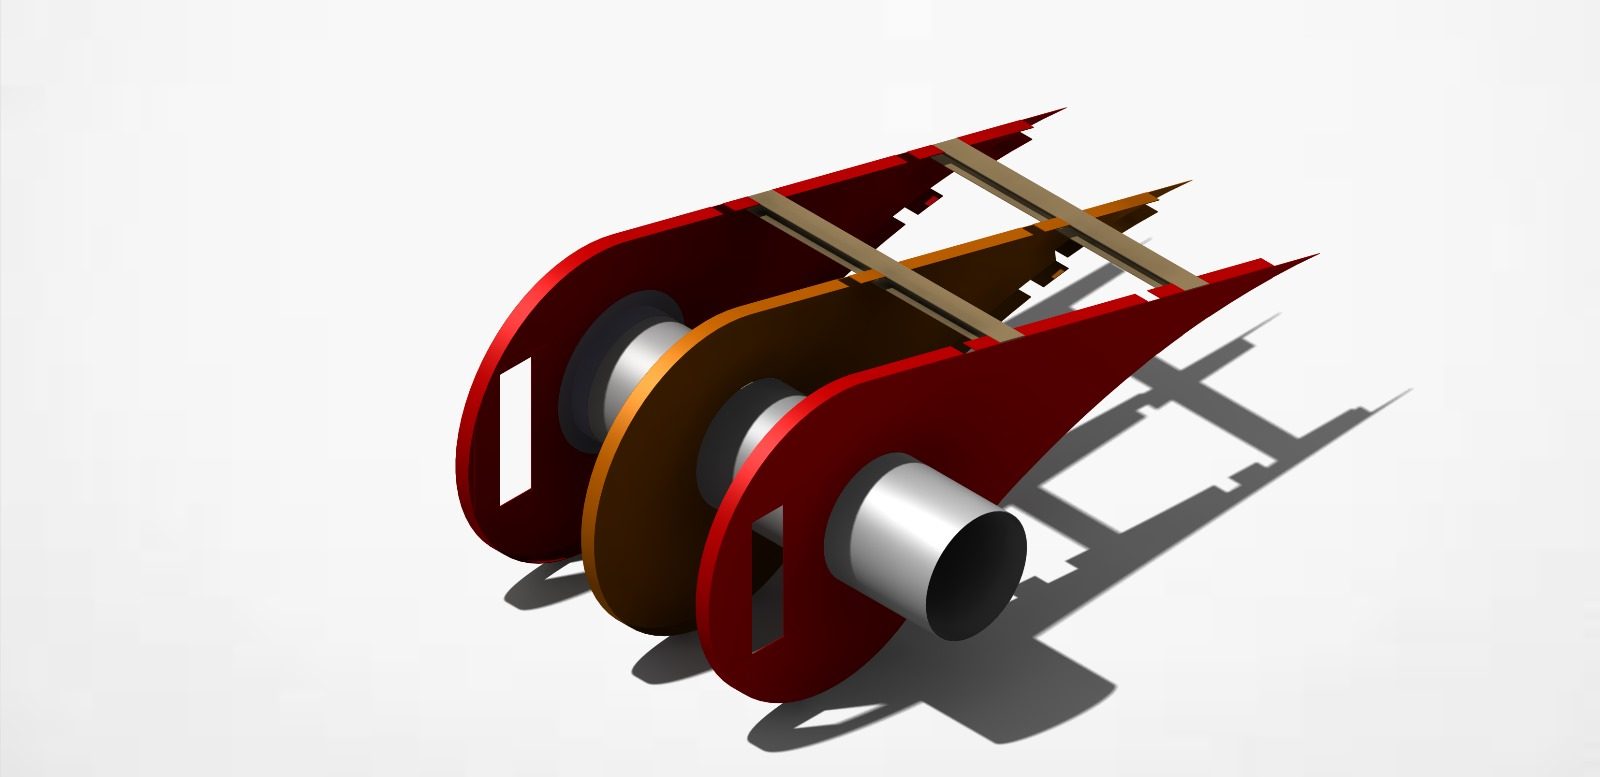
\includegraphics[width=2cm]{Figures/Montaje/8.jpg}}; & \\  \node[lablum=i]{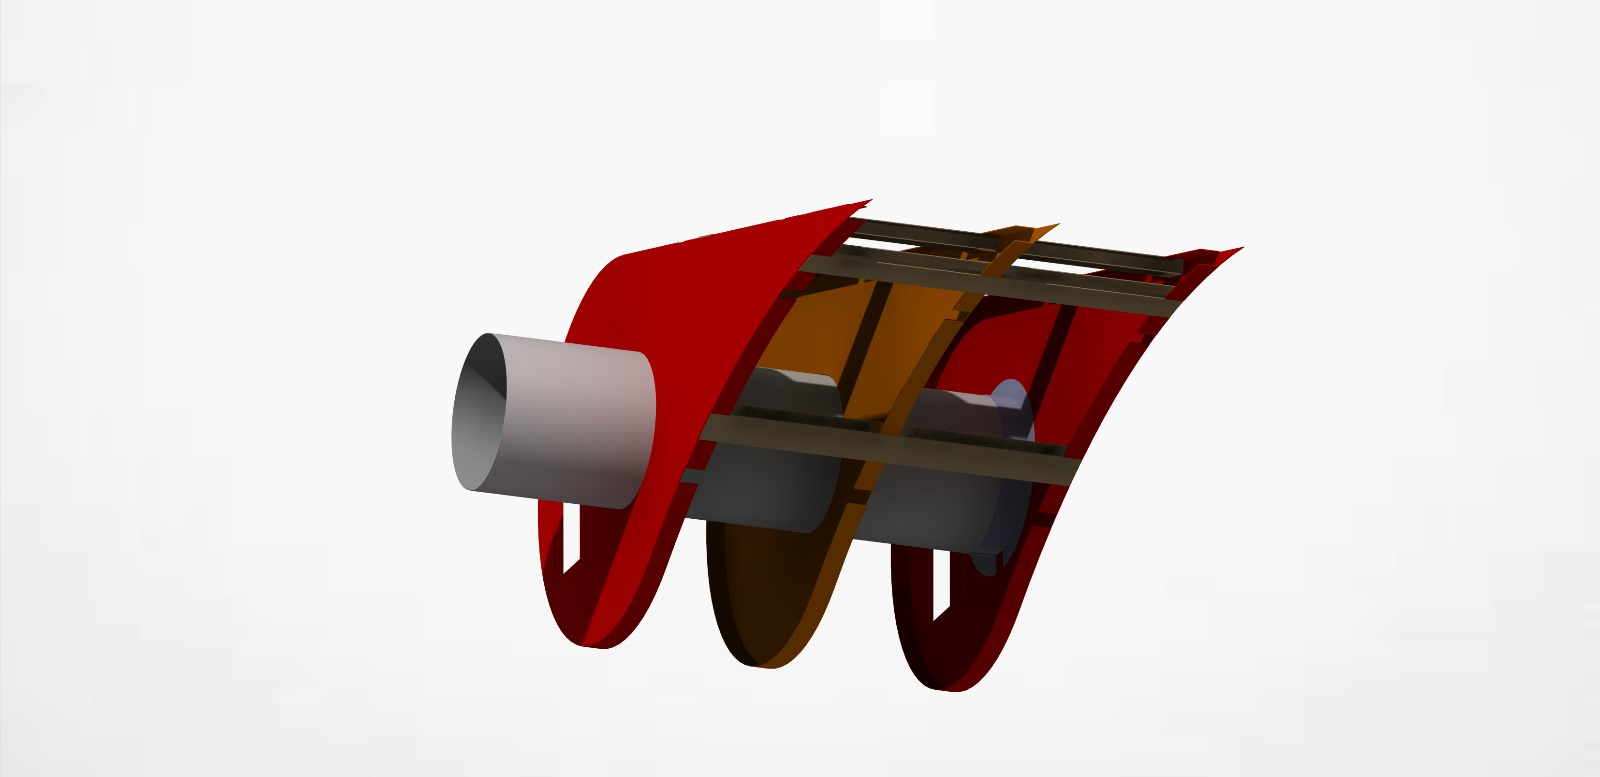
\includegraphics[width=5.5cm]{Figures/Montaje/9.jpg}}; & \node[lablum=j]{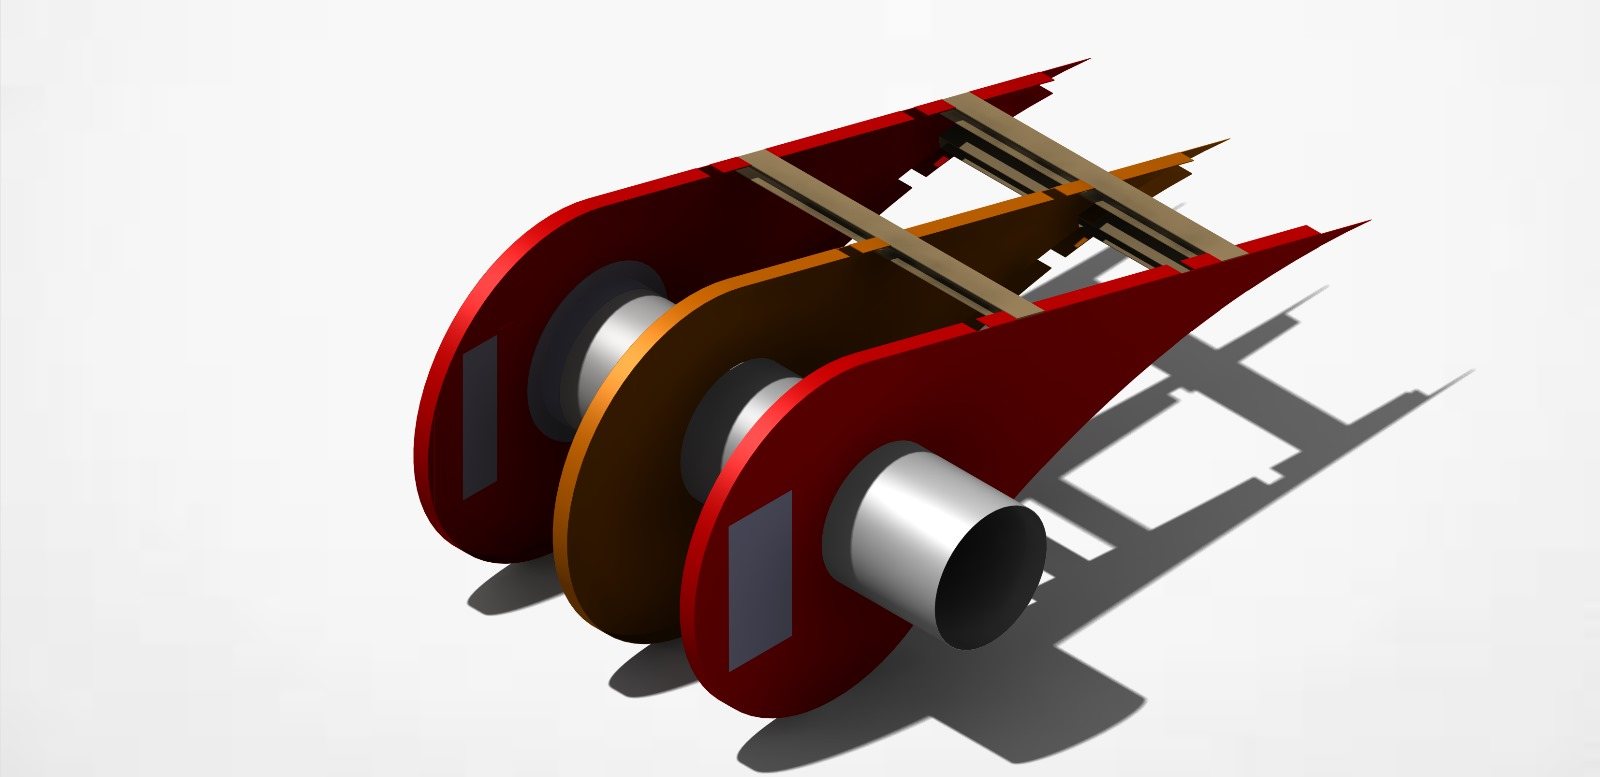
\includegraphics[width=2cm]{Figures/Montaje/10.jpg}}; \\
 };
\draw[marr] ([xshift=1mm]img-h.south west) coordinate (aux) 
 -- (img-i.north-|aux);
 \draw[marr] (img-i) -- (img-j);
\end{tikzpicture}
\caption{Noveno Paso. \label{fig:nov}}
\end{figure}
%===============================================================================================================
\pagebreak
\subsection{Décimo Paso: Tapa de Acceso}
Este proceso se realizará tanto para la costilla trasera como para la trasera.

La tapa de acceso, de dimensiones 180$\times$90, se unirá a la costilla mediante un remachado visible con cabeza universal, que se podrá quitar para acceder a la estructura interior. La estructura ha de estar levemente hundida para que, cuando se remache, quede lisa, y no afecta al comportamiento aerodinámico.

Con un granete se marca la pieza y, posteriormente, se taladra. Se pinza para sujetar los remaches en su lugar, mientras se aplica la fuerza para fijarlos. Una vez remachado, se efectúa el avellanado.

Ver figura \ref{fig:dec}.

%===============================================================================================================
%                                                   DÉCIMO PASO
%===============================================================================================================
\begin{figure}[!htb]
\centering
\begin{tikzpicture}[lablum/.style 2 args={label=below:#1 #2,name=img-#1},
marr/.style={line width=1mm,-latex}]
 \matrix[column sep=1cm,row sep=5mm] (mat)
 { \node[lablum=i]{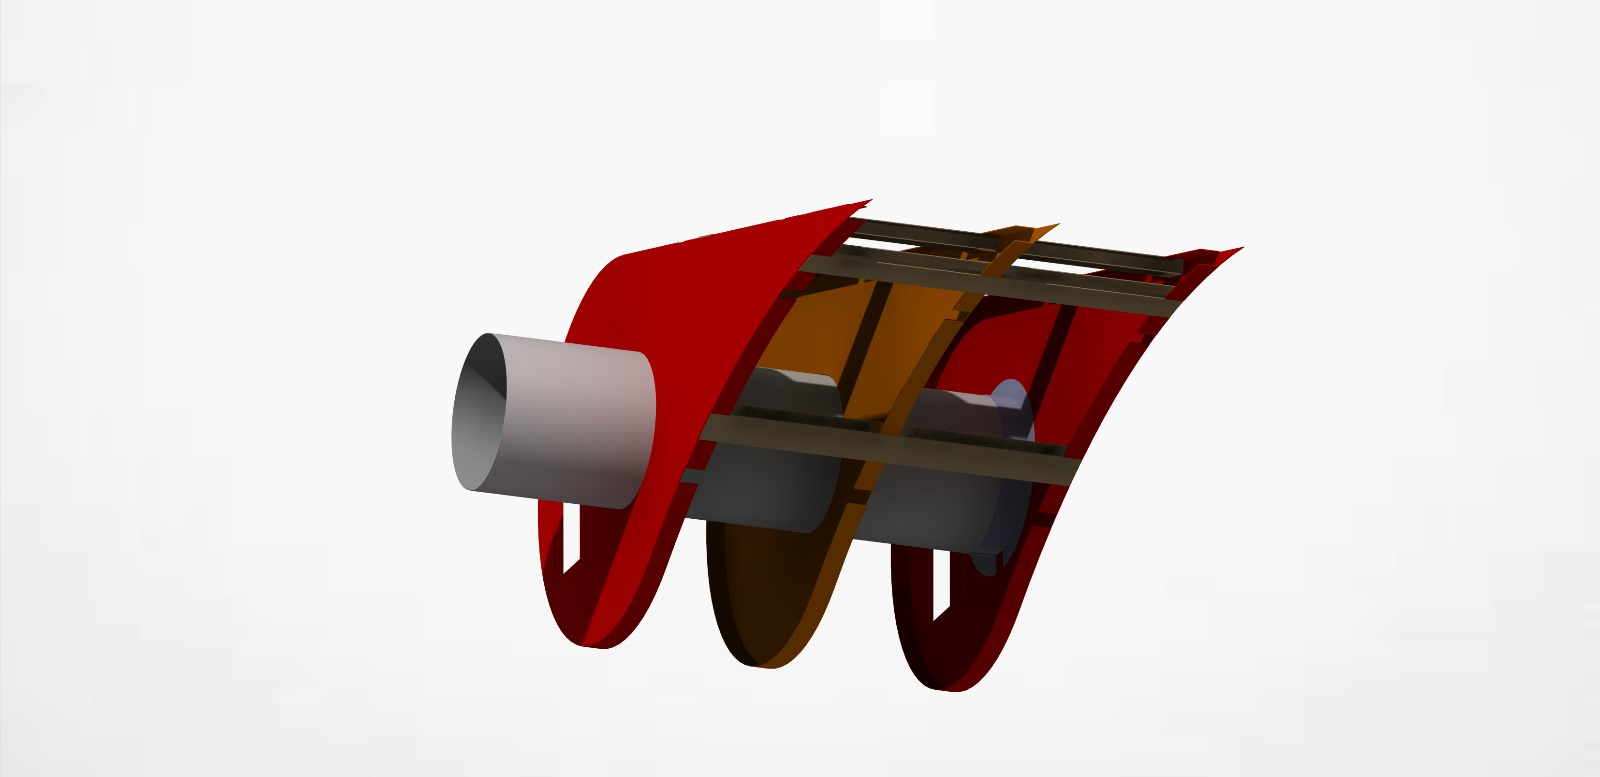
\includegraphics[width=2cm]{Figures/Montaje/9.jpg}}; & \node[lablum=j]{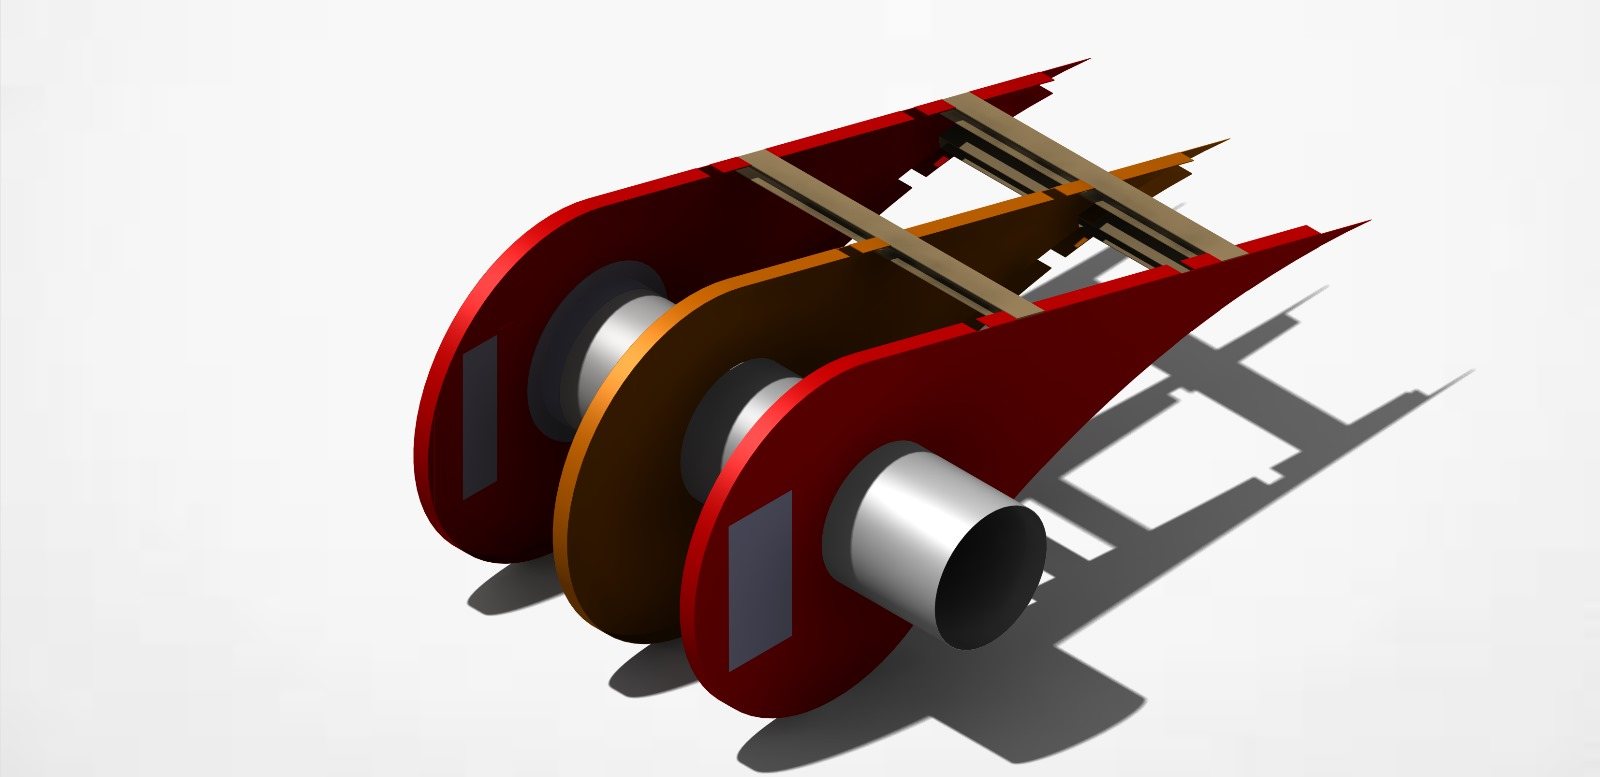
\includegraphics[width=5.5cm]{Figures/Montaje/10.jpg}}; \\ 
 & \node[lablum=k]{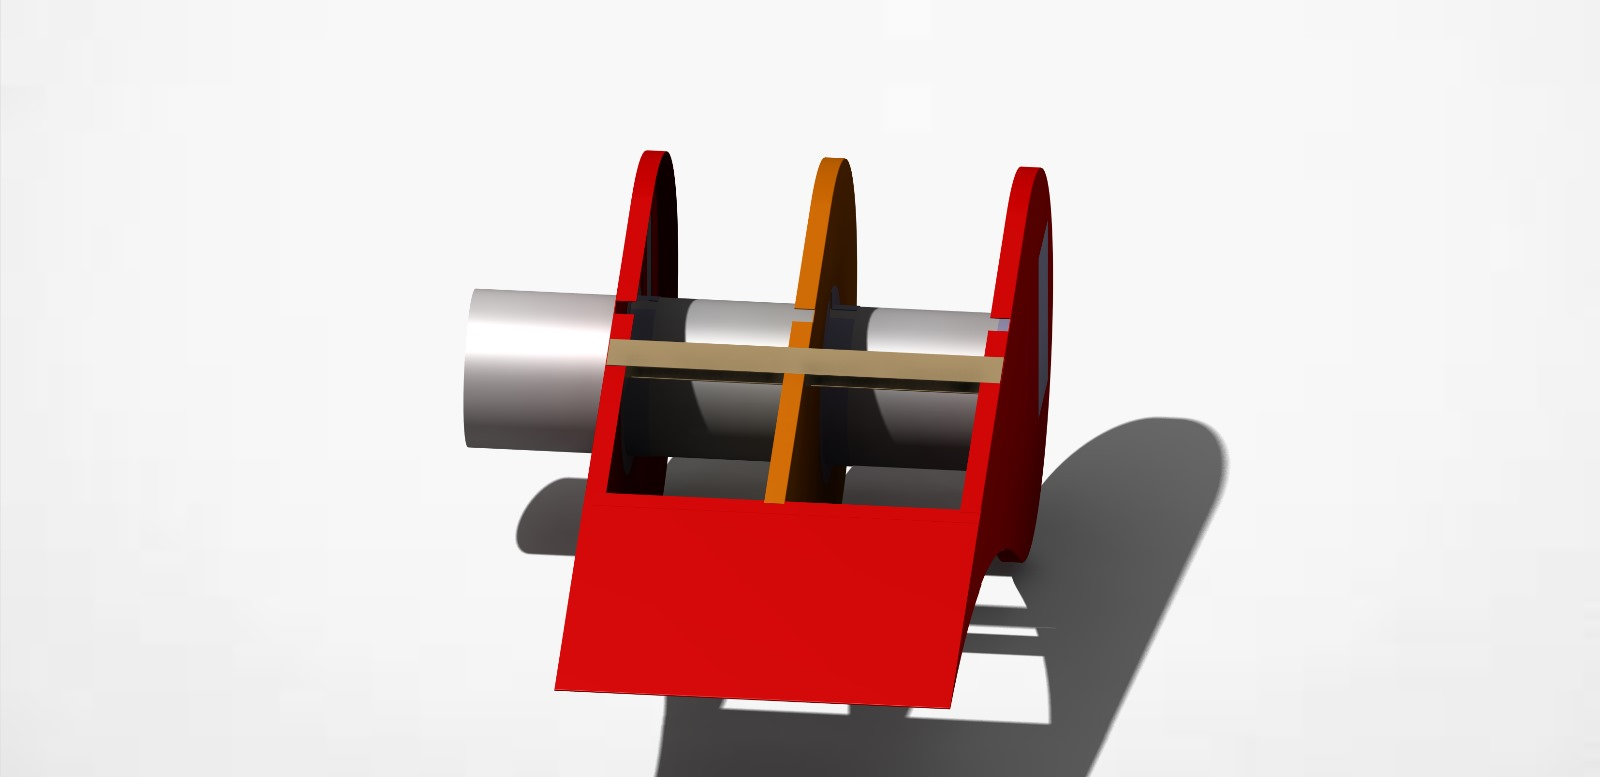
\includegraphics[width=2cm]{Figures/Montaje/11.jpg}}; \\
 };
 \draw[marr] (img-i) -- (img-j);
  \draw[marr] ([xshift=-1mm]img-j.south east) coordinate (aux) 
 -- (img-k.north-|aux);
\end{tikzpicture}
\caption{Décimo Paso. \label{fig:dec}}
\end{figure}
%===============================================================================================================


\subsection{Undécimo Paso: Revestimiento del Borde de Salida}
Colocamos el primer revestimiento, que ha sido moldeado para que adquiera la forma del borde de salida, y que, además, cuenta con los extremos doblados para que se introduzca a las ranuras de la costilla.

Como la soldadura no es conveniente aquí (produce una deformación indeseada), el proceso se realizará mediante remachado ciego, con posterior avellanado, a fin de evitar que la cabeza sobresalga de la superficie. 

El remachado ha sido explicado en detalle en el paso anterior.

Ver figura \ref{fig:und}.

%===============================================================================================================
%                                                  11º PASO
%===============================================================================================================
\begin{figure}[!htb]
\centering
\begin{tikzpicture}[lablum/.style 2 args={label=below:#1 #2,name=img-#1},
marr/.style={line width=1mm,-latex}]
 \matrix[column sep=1cm,row sep=5mm] (mat)
 { & \node[lablum=j]{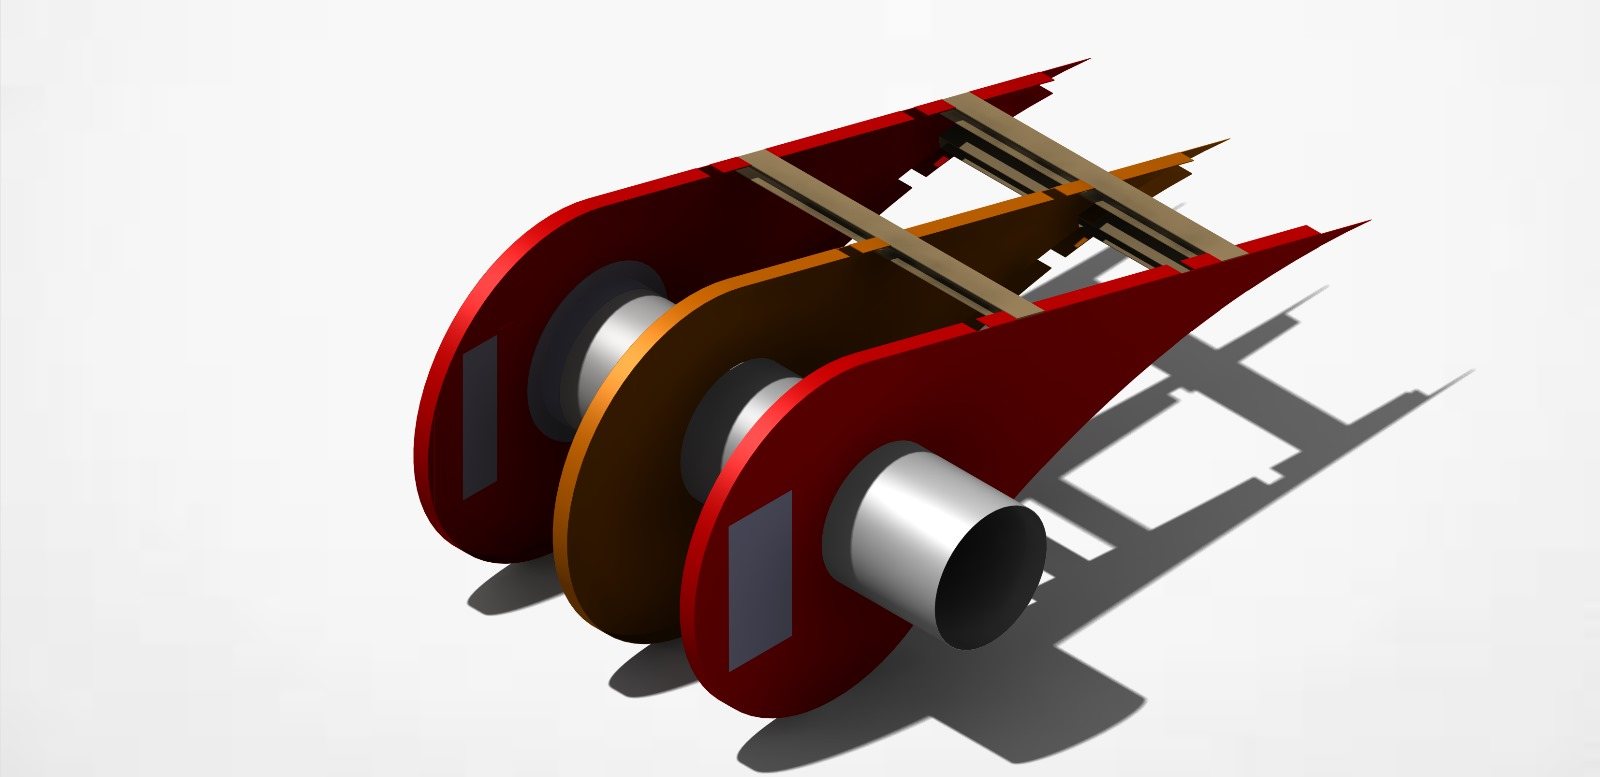
\includegraphics[width=2cm]{Figures/Montaje/10.jpg}}; \\ 
\node[lablum=l]{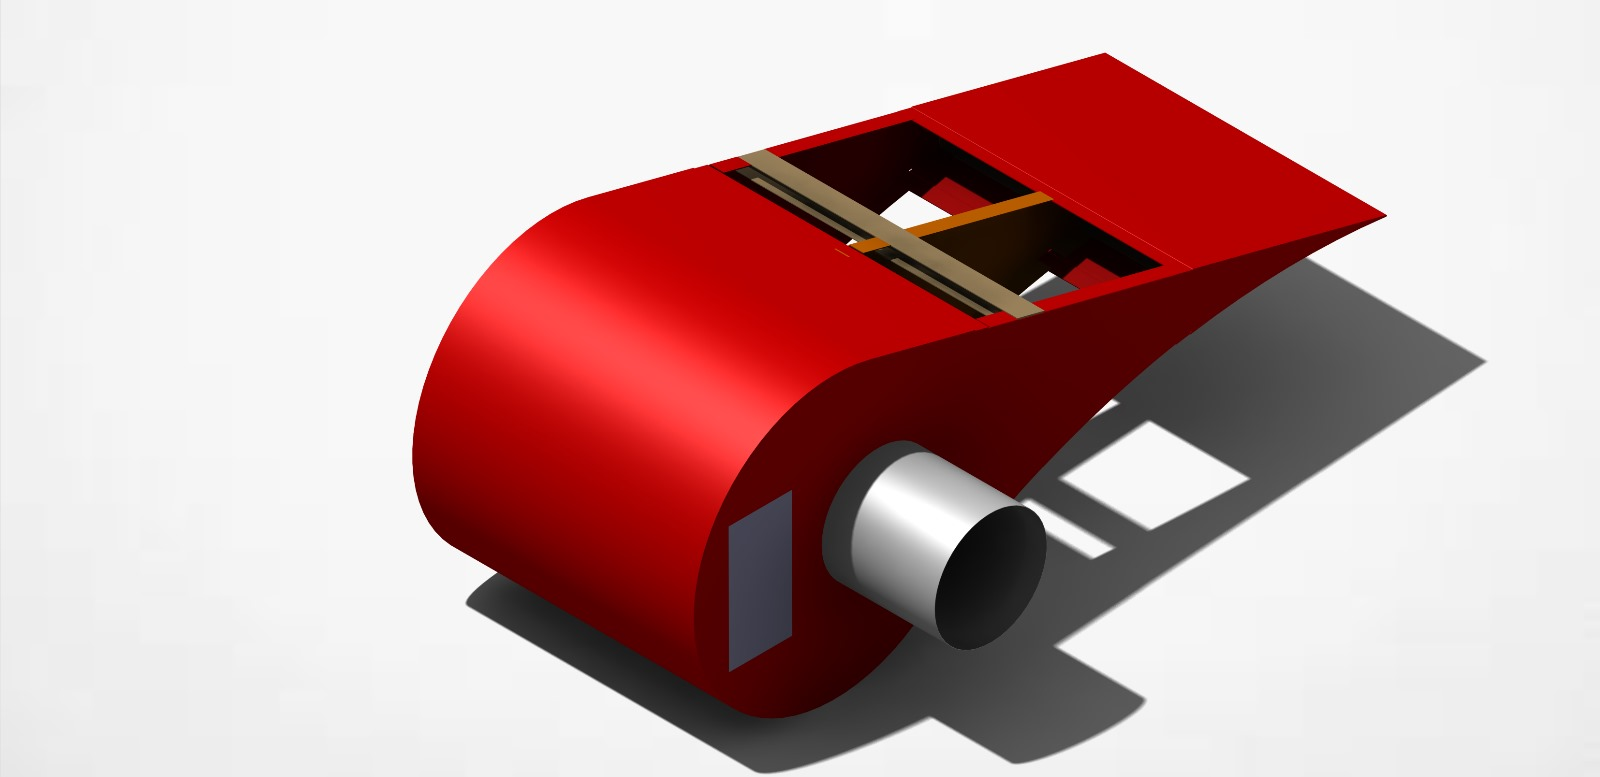
\includegraphics[width=2cm]{Figures/Montaje/12.jpg}}; & \node[lablum=k]{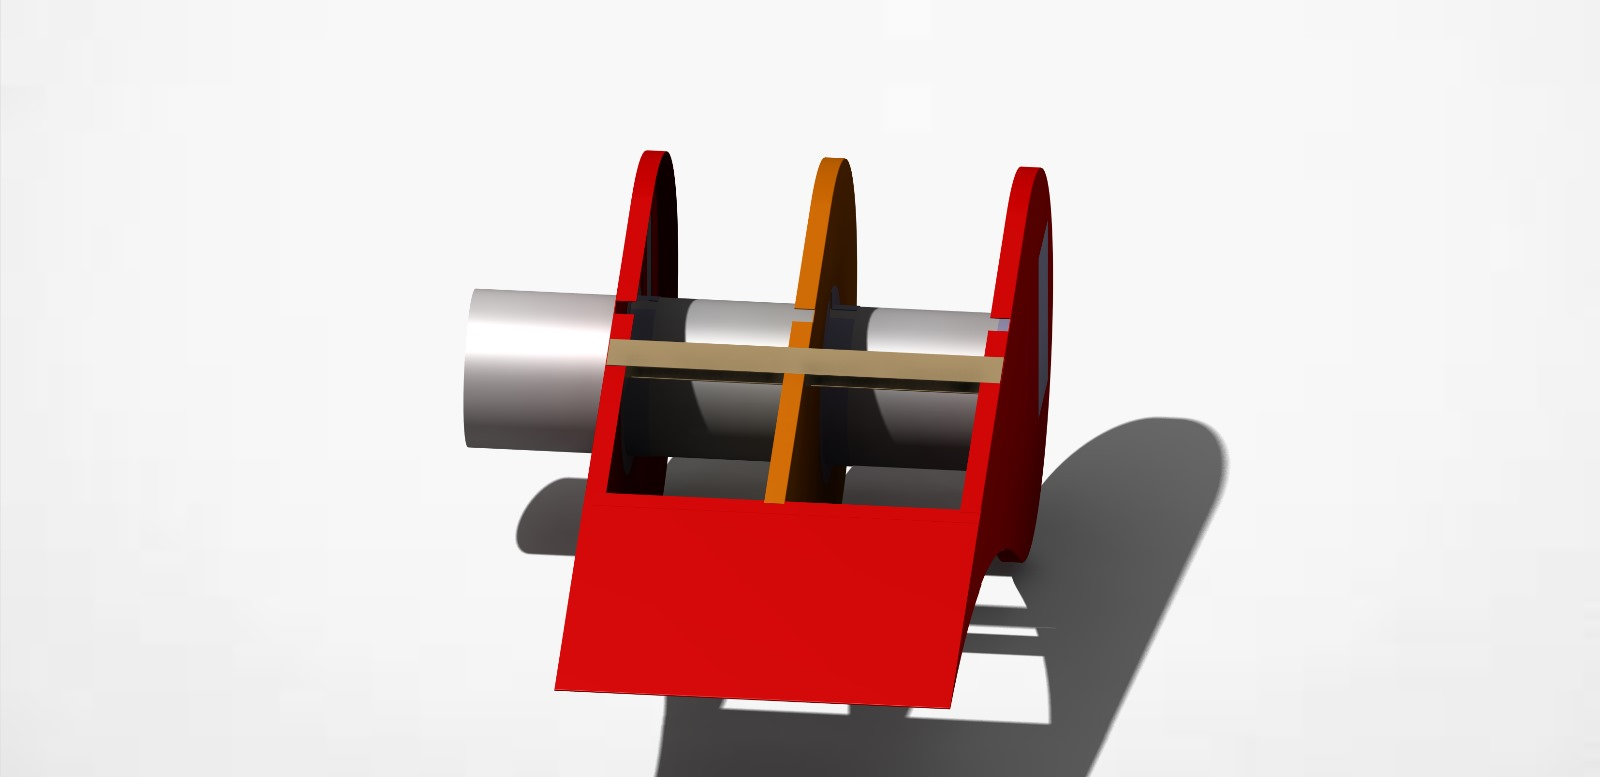
\includegraphics[width=5.5cm]{Figures/Montaje/11.jpg}}; \\
 };
\draw[marr] ([xshift=-1mm]img-j.south east) coordinate (aux) 
 -- (img-k.north-|aux);
  \draw[marr] (img-k) -- (img-l);
\end{tikzpicture}
\caption{Undécimo Paso. \label{fig:und}}
\end{figure}
%===============================================================================================================

\subsection{Duodécimo Paso: Revestimiento del Borde de Ataque}
Análogo al paso anterior. Colocamos el revestimiento, que ha sido moldeado con forma del borde de ataque, siguiendo el procedimiento descrito en el paso anterior.

Ver figura \ref{fig:duo}.

%===============================================================================================================
%                                                   12º PASO
%===============================================================================================================
\begin{figure}[!htb]
\centering
\begin{tikzpicture}[lablum/.style 2 args={label=below:#1 #2,name=img-#1},
marr/.style={line width=1mm,-latex}]
 \matrix[column sep=1cm,row sep=5mm] (mat)
 { \node[lablum=l]{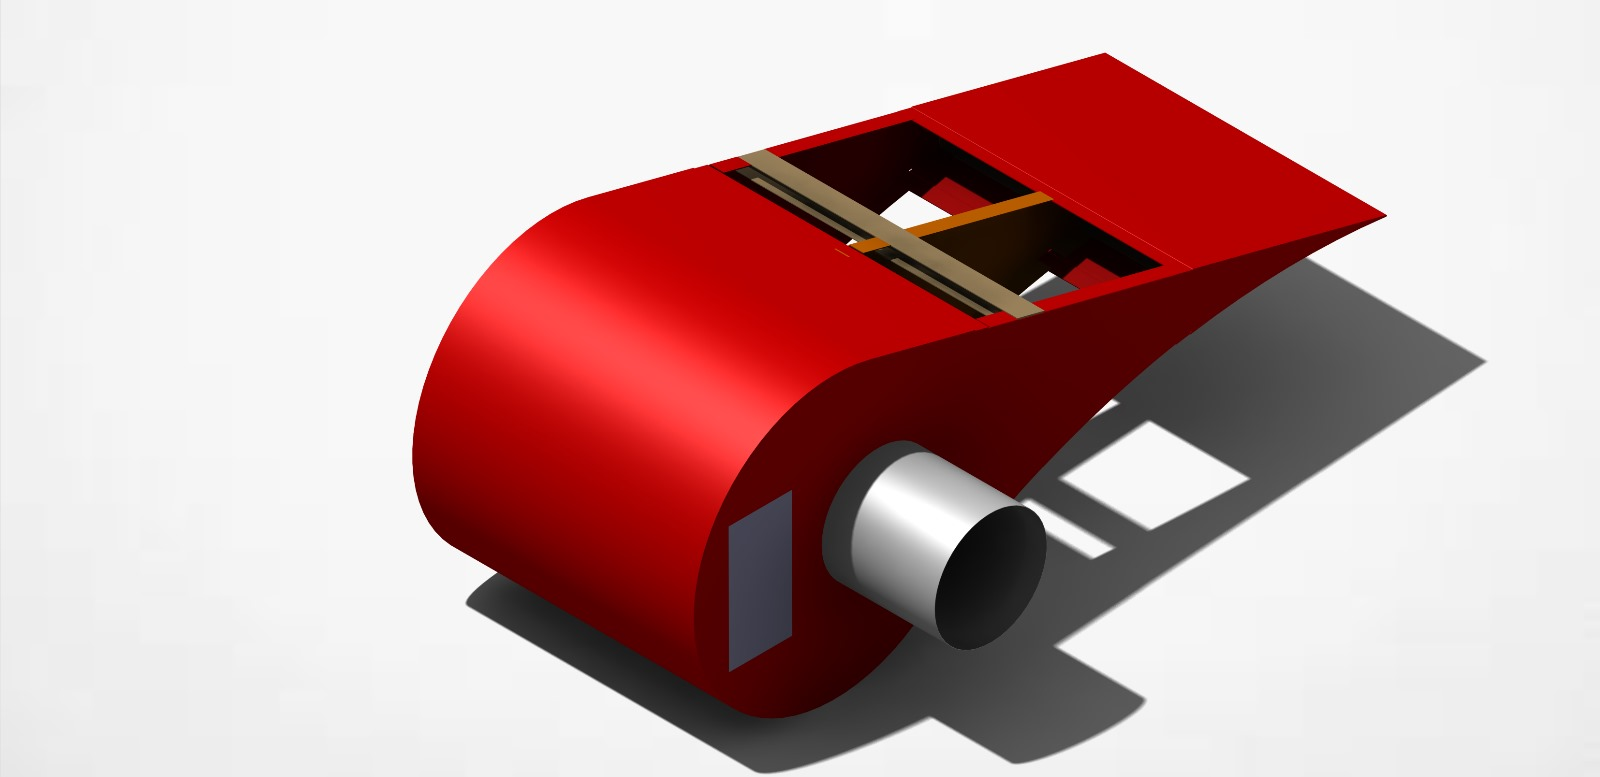
\includegraphics[width=5.5cm]{Figures/Montaje/12.jpg}}; & \node[lablum=k]{\includegraphics[width=2cm]{Figures/Montaje/11.jpg}}; \\
 \node[lablum=m]{\includegraphics[width=2cm]{Figures/Montaje/13.jpg}}; &  \\
 };
\draw[marr] (img-k) -- (img-l);
\draw[marr] ([xshift=1mm]img-l.south west) coordinate (aux) 
 -- (img-m.north-|aux);
\end{tikzpicture}
\caption{Duodécimo Paso.\label{fig:duo}}
\end{figure}
%===============================================================================================================


\subsection{Decimotercer Paso: Revestimiento del Extradós}
Se efectúa un remachado de caña maciza con avellanado posterior. Como el revestimiento del intradós aún no ha sido colocado, tenemos acceso en sendas partes, por lo que podemos realizar un remachado no ciego.

Ver figura \ref{fig:dete}.

%===============================================================================================================
%                                                   13º PASO
%===============================================================================================================
\begin{figure}[!htb]
\centering
\begin{tikzpicture}[lablum/.style 2 args={label=below:#1 #2,name=img-#1},
marr/.style={line width=1mm,-latex}]
 \matrix[column sep=1cm,row sep=5mm] (mat)
 { \node[lablum=l]{\includegraphics[width=2cm]{Figures/Montaje/12.jpg}}; &  \\
 \node[lablum=m]{\includegraphics[width=5.5cm]{Figures/Montaje/13.jpg}}; & \node[lablum=n]{\includegraphics[width=2cm]{Figures/Montaje/14.jpg}}; \\
 };
\draw[marr] ([xshift=1mm]img-l.south west) coordinate (aux) 
 -- (img-m.north-|aux);
\draw[marr] (img-m) -- (img-n);
\end{tikzpicture}
\caption{Decimotercer Paso. \label{fig:dete}}
\end{figure}
%===============================================================================================================


\subsection{Decimocuarto paso: Revestimiento del Intradós}
El procedimiento del paso anterior se repite para el intradós, pero procediendo con un remachado ciego, al no contar con acceso por las dos partes.

Ver figura \ref{fig:decic}.
%===============================================================================================================
%                                                   14º PASO
%===============================================================================================================
\begin{figure}[!htb]
\centering
\begin{tikzpicture}[lablum/.style 2 args={label=below:#1 #2,name=img-#1},
marr/.style={line width=1mm,-latex}]
 \matrix[column sep=1cm,row sep=5mm] (mat)
 { \node[lablum=l]{\includegraphics[width=2cm]{Figures/Montaje/12.jpg}}; &  \\
 \node[lablum=m]{\includegraphics[width=2cm]{Figures/Montaje/13.jpg}}; & \node[lablum=n]{\includegraphics[width=5.5cm]{Figures/Montaje/14.jpg}}; \\
 };
\draw[marr] ([xshift=1mm]img-l.south west) coordinate (aux) 
 -- (img-m.north-|aux);
\draw[marr] (img-m) -- (img-n);
\end{tikzpicture}
\caption{Decimocuarto Paso. \label{fig:decic}}
\end{figure}
%===============================================================================================================

\section{Proceso Global}
El proceso global se detalla en la figura \ref{fig:montaje}

%===============================================================================================================
%                                                   PROCESO GLOBAL
%===============================================================================================================
\begin{figure}[!htb]
\centering
\begin{tikzpicture}[lablum/.style 2 args={label=below:#1 #2,name=img-#1},
marr/.style={line width=1mm,-latex}]
 \matrix[column sep=1cm,row sep=5mm] (mat)
 { \node[lablum={a}{}]{\includegraphics[width=4cm]{Figures/Montaje/1.jpg}};
 & \node[lablum={b}{}]{\includegraphics[width=4cm]{Figures/Montaje/2.jpg}};\\
 \node[lablum=d]{\includegraphics[width=4cm]{Figures/Montaje/4.jpg}};
 & \node[lablum=c]{\includegraphics[width=4cm]{Figures/Montaje/3.jpg}};\\
 \node[lablum=e]{\includegraphics[width=4cm]{Figures/Montaje/5.jpg}};
 & \node[lablum=f]{\includegraphics[width=4cm]{Figures/Montaje/6.jpg}};\\
 \node[lablum=h]{\includegraphics[width=4cm]{Figures/Montaje/8.jpg}}; & \node[lablum=g]{\includegraphics[width=4cm]{Figures/Montaje/7.jpg}};\\ 
\node[lablum=i]{\includegraphics[width=4cm]{Figures/Montaje/9.jpg}}; & \node[lablum=j]{\includegraphics[width=4cm]{Figures/Montaje/10.jpg}}; \\
\node[lablum=l]{\includegraphics[width=4cm]{Figures/Montaje/12.jpg}}; & \node[lablum=k]{\includegraphics[width=4cm]{Figures/Montaje/11.jpg}}; \\
\node[lablum=m]{\includegraphics[width=4cm]{Figures/Montaje/13.jpg}}; & \node[lablum=n]{\includegraphics[width=4cm]{Figures/Montaje/14.jpg}}; \\
 };
 % -------------------------------------------------
 \draw[marr] (img-a) -- (img-b);
 \draw[marr] ([xshift=1mm]img-b.south east) coordinate (aux) 
 -- (img-c.north-|aux);
 \draw[marr] (img-c) -- (img-d);
 \draw[marr] ([xshift=-1mm]img-d.south west) coordinate (aux) 
 -- (img-e.north-|aux);
 \draw[marr] (img-e) -- (img-f);
 \draw[marr] ([xshift=-1mm]img-f.south east) coordinate (aux) 
 -- (img-g.north-|aux);
\draw[marr] (img-g) -- (img-h);
 \draw[marr] ([xshift=1mm]img-h.south west) coordinate (aux) 
 -- (img-i.north-|aux);
\draw[marr] (img-i) -- (img-j);
 \draw[marr] ([xshift=-1mm]img-j.south east) coordinate (aux) 
 -- (img-k.north-|aux);
 \draw[marr] (img-k) -- (img-l);
  \draw[marr] ([xshift=1mm]img-l.south west) coordinate (aux) 
 -- (img-m.north-|aux);
 \draw[marr] (img-m) -- (img-n);
\end{tikzpicture}
\caption{Proceso de Montaje.  \label{fig:montaje}}
\end{figure}
%===============================================================================================================
\cleardoublepage



%   ---   BIBLIOGRAFÍA/REFERENCIAS   ---   %

\phantomsection
\addcontentsline{toc}{section}{Referencias}
\renewcommand{\refname}{Referencias}
\bibliographystyle{elsarticle-num}
\bibliography{references.bib}
\cleardoublepage



%   ---   ANEXOS   ---   %

\appendix
\renewcommand{\appendixname}{Anexo}
\addcontentsline{toc}{section}{\appendixname}
\cleardoublepage
\appendixpage
\addappheadtotoc
\renewcommand{\appendixname}{Anexo}

\includepdf{Figures/Enunciado/plano.pdf}
\cleardoublepage





\end{document}